% **************************************************
% Document Class Definition
% **************************************************
\documentclass[%
	paper=A4,					% paper size --> A4 is default in Germany
	twoside=true,				% onesite or twoside printing
	openright,					% doublepage cleaning ends up right side
	parskip=full,				% spacing value / method for paragraphs
	chapterprefix=true,			% prefix for chapter marks
	11pt,						% font size
	headings=normal,			% size of headings
	bibliography=totoc,			% include bib in toc
	listof=totoc,				% include listof entries in toc
	titlepage=on,				% own page for each title page
	captions=tableabove,		% display table captions above the float env
	draft=false,				% value for draft version
]{scrreprt}%

% **************************************************
% Debug LaTeX Information
% **************************************************
%\listfiles

% **************************************************
% Information and Commands for Reuse
% **************************************************
\newcommand{\thesisTitle}{Automated Test Generation for
for production systems in a Model-based Testing approach.}
\newcommand{\thesisName}{William Durand}
\newcommand{\thesisSubject}{Documentation}
\newcommand{\thesisDate}{\today}
\newcommand{\thesisVersion}{draft}

\newcommand{\thesisFirstReviewer}{Jane git stDoe}
\newcommand{\thesisFirstReviewerUniversity}{\protect{Clean Thesis Style University}}
\newcommand{\thesisFirstReviewerDepartment}{Department of Clean Thesis Style}

\newcommand{\thesisSecondReviewer}{John Doe}
\newcommand{\thesisSecondReviewerUniversity}{\protect{Clean Thesis Style University}}
\newcommand{\thesisSecondReviewerDepartment}{Department of Clean Thesis Style}

\newcommand{\thesisFirstSupervisor}{S\'ebastien Salva}
\newcommand{\thesisSecondSupervisor}{Patrice Lauren\c{c}ot}

\newcommand{\thesisUniversity}{\protect{Universit\'e Blaise Pascal}}
\newcommand{\thesisUniversityDepartment}{LIMOS - UMR 6158}
\newcommand{\thesisUniversityInstitute}{}
\newcommand{\thesisUniversityGroup}{}
\newcommand{\thesisUniversityCity}{Aubi\`ere, France}
\newcommand{\thesisUniversityStreetAddress}{Campus Universitaire
des C\'ezeaux - 1 rue de la Chebarde}
\newcommand{\thesisUniversityPostalCode}{63178}

% **************************************************
% Load and Configure Packages
% **************************************************
\usepackage[utf8]{inputenc}		% defines file's character encoding
\usepackage[english]{babel} % babel system, adjust the language of the content
\usepackage[					% clean thesis style
	figuresep=colon,
	sansserif=false,
	hangfigurecaption=false,
	hangsection=true,
	hangsubsection=true,
	colorize=full,
	colortheme=bluemagenta,
	bibsys=bibtex,
	bibfile=bib-refs,
    bibstyle=alphabetic,
]{cleanthesis}

\hypersetup{					% setup the hyperref-package options
	pdftitle={\thesisTitle},	% 	- title (PDF meta)
	pdfsubject={\thesisSubject},% 	- subject (PDF meta)
	pdfauthor={\thesisName},	% 	- author (PDF meta)
	plainpages=false,			% 	-
	colorlinks=false,			% 	- colorize links?
	pdfborder={0 0 0},			% 	-
	breaklinks=true,			% 	- allow line break inside links
	bookmarksnumbered=true,		%
	bookmarksopen=true			%
}

% My packages
\usepackage{euscript}
\usepackage{listings}
\usepackage[lofdepth,lotdepth]{subfig}
\usepackage[ruled,vlined,linesnumbered]{algorithm2e}
\usepackage{mathtools}
\usepackage{comment}
\usepackage{verbatim}
\usepackage{float}
\usepackage{color}
\usepackage{theorem}
\usepackage{amsfonts} % for \mathbb
\usepackage{stmaryrd} % for \llbracket
\usepackage{framed}   % for \begin{framed}
\usepackage{fancyvrb} % for \begin{BVerbatim}
\usepackage{hyperref} % for clickable refs

% My commands
\newcommand{\R}{\mathbb{R}}
\newcommand{\N}{\mathbb{N}}
\newtheorem{theorem}{Theorem}
\newtheorem{definition}[theorem]{Definition}
\newtheorem{proposition}[theorem]{Proposition}
\newtheorem{remark}[theorem]{Remark}
\newtheorem{theoremLem}{Theorem}
\newtheorem{lemma}[theoremLem]{Lemma}

\newcounter{example}[section]
\def\theexample{\thesection.\arabic{example}}
\newenvironment{example}[1][]
{\refstepcounter{example}
\medskip\noindent{\bfseries Example \theexample\ #1\,\,\,}}
{\medskip}

% **************************************************
% Document CONTENT
% **************************************************
\begin{document}

% --------------------------
% rename document parts
% --------------------------
%\renewcaptionname{ngerman}{\figurename}{Abb.}
%\renewcaptionname{ngerman}{\tablename}{Tab.}
\renewcaptionname{english}{\figurename}{Fig.}
\renewcaptionname{english}{\tablename}{Tab.}

% --------------------------
% Front matter
% --------------------------
\pagenumbering{roman}			% roman page numbing (invisible for empty page style)
\pagestyle{empty}				% no header or footers
% !TEX root = ../thesis.tex
%
% ------------------------------------  --> cover title page
\begin{titlepage}
	\pdfbookmark[0]{Cover}{Cover}
	\flushright
	\hfill
	\vfill
	{\LARGE\thesisTitle \par}
	\rule[5pt]{\textwidth}{.4pt} \par
	{\Large\thesisName}
	\vfill
	\textit{\large\thesisDate} \\
	Version: \thesisVersion
\end{titlepage}


% ------------------------------------  --> main title page
\begin{titlepage}
	\pdfbookmark[0]{Titlepage}{Titlepage}
	\tgherosfont
	\centering

	{\Large \thesisUniversity} \\[4mm]
	\textsf{\thesisUniversityDepartment} \\
	\textsf{\thesisUniversityInstitute} \\
	\textsf{\thesisUniversityGroup} \\

	\vfill
	{\large \thesisSubject} \\[5mm]
	{\LARGE \color{ctcolortitle}\textbf{\thesisTitle} \\[10mm]}
	{\Large \thesisName} \\

	\vfill
	\begin{minipage}[t]{.27\textwidth}
		\raggedleft
		\textit{1. Reviewer}
	\end{minipage}
	\hspace*{15pt}
	\begin{minipage}[t]{.65\textwidth}
		{\Large \thesisFirstReviewer} \\
	  	{\small \thesisFirstReviewerDepartment} \\[-1mm]
		{\small \thesisFirstReviewerUniversity}
	\end{minipage} \\[5mm]
	\begin{minipage}[t]{.27\textwidth}
		\raggedleft
		\textit{2. Reviewer}
	\end{minipage}
	\hspace*{15pt}
	\begin{minipage}[t]{.65\textwidth}
		{\Large \thesisSecondReviewer} \\
	  	{\small \thesisSecondReviewerDepartment} \\[-1mm]
		{\small \thesisSecondReviewerUniversity}
	\end{minipage} \\[10mm]
	\begin{minipage}[t]{.27\textwidth}
		\raggedleft
		\textit{Supervisors}
	\end{minipage}
	\hspace*{15pt}
	\begin{minipage}[t]{.65\textwidth}
		\thesisFirstSupervisor\ and \thesisSecondSupervisor
	\end{minipage} \\[10mm]

	\thesisDate \\

\end{titlepage}


% ------------------------------------  --> lower title back for single page layout
\hfill
\vfill
{
	\small
	\textbf{\thesisName} \\
	\textit{\thesisTitle} \\
	\thesisSubject, \thesisDate \\
	Reviewers: \thesisFirstReviewer\ and \thesisSecondReviewer \\
	Supervisors: \thesisFirstSupervisor\ and \thesisSecondSupervisor \\[1.5em]
	\textbf{\thesisUniversity} \\
	\textit{\thesisUniversityGroup} \\
	\thesisUniversityInstitute \\
	\thesisUniversityDepartment \\
	\thesisUniversityStreetAddress \\
	\thesisUniversityPostalCode\ and \thesisUniversityCity
}
		    % INCLUDE: all titlepages
\cleardoublepage

\pagestyle{plain}				% display just page numbers
% !TEX root = ../thesis.tex
%
\pdfbookmark[0]{Abstract}{Abstract}
\chapter*{Abstract}
\label{sec:abstract}
\vspace*{-10mm}

\blindtext

\vspace*{20mm}

{\usekomafont{chapter}Abstract (different language)}\label{sec:abstract-diff} \\

\blindtext
		    % INCLUDE: the abstracts (english and german)
\cleardoublepage
%
% !TEX root = ../thesis.tex
%
\pdfbookmark[0]{Acknowledgement}{Acknowledgement}
\chapter*{Acknowledgement}
\label{sec:acknowledgement}
\vspace*{-10mm}

\TODO{to write}
     % INCLUDE: acknowledgement
\cleardoublepage
%
\setcounter{tocdepth}{3}		% define depth of toc
\tableofcontents				% display table of contents
\cleardoublepage

% --------------------------
% Body matter
% --------------------------
\pagenumbering{arabic}			% arabic page numbering
\setcounter{page}{1}			% set page counter
\pagestyle{maincontentstyle} 	% fancy header and footer

% !TEX root = ../../thesis.tex
%
\chapter{Introduction}
\label{sec:intro}

\cleanchapterquote{You can’t do better design with a computer, but you can speed up your work enormously.}{Wim Crouwel}{(Graphic designer and typographer)}

\Blindtext[2][2]

\section{Postcards: My Address}
\label{sec:intro:address}

\textbf{Ricardo Langner} \\
Alfred-Schrapel-Str. 7 \\
01307 Dresden \\
Germany


\section{Motivation and Problem Statement}
\label{sec:intro:motivation}

\Blindtext[3][1] \cite{Jurgens:2000,Jurgens:1995,Miede:2011,Kohm:2011,Apple:keynote:2010,Apple:numbers:2010,Apple:pages:2010}

\section{Results}
\label{sec:intro:results}

\Blindtext[1][2]

\subsection{Some References}
\label{sec:intro:results:refs}
\cite{WEB:GNU:GPL:2010,WEB:Miede:2011}

\section{Thesis Structure}
\label{sec:intro:structure}

\textbf{Chapter \ref{sec:related}} \\[0.2em]
\blindtext

\textbf{Chapter \ref{sec:system}} \\[0.2em]
\blindtext

\textbf{Chapter \ref{sec:concepts}} \\[0.2em]
\blindtext

\textbf{Chapter \ref{sec:concepts}} \\[0.2em]
\blindtext

\textbf{Chapter \ref{sec:conclusion}} \\[0.2em]
\blindtext

% !TEX root = ../../thesis.tex
%
\chapter{Definitions and notations}
\label{sec:definitions}

%%%%%%%%%%%%%%%%%%%%%%%%%%%%%%%%%%%%%%%%%%%%%%%%%%%%%%%%%%%%%%%%%

\section{Symbolic Transition Systems}
\label{sec:definitions:sts}

The \textit{Symbolic Transition System} (STS) is known as a very
general and powerful model for describing several aspects of
event-based systems. The use of symbolic variables helps describe
infinite state machines in a finite manner. This potentially
infinite behaviour is represented by the semantics of a STS,
given in terms of \textit{Labelled Transition System} (LTS). STS
operations and transformations are often given with inference
rules.

We briefly give some definitions related to the STS model below,
but we refer to \cite{FTW05} for a more detailed description.

\begin{definition}[Variable assignment]
We assume that there exist a domain of values denoted $D$ and a
variable set $X$ taking values in $D$. The assignment of
variables in $Y \subseteq X$ to elements of $D$ is denoted with a
mapping  $\alpha: Y \rightarrow D$.

We denote $D_Y$ the assignment set over $Y$. We also denote
$id_Y$ the identity assignment over $Y$, and $v_\emptyset$ the
empty assignment.
\end{definition}

\begin{definition}[STS]
    A Symbolic Transition System (STS) is a tuple
    $<L,l_0,V,V_0,I,\Lambda,\rightarrow>$, where:

	\begin{itemize}
        \item STSs do not have states but locations and $L$ is
        the finite location set, with $l_0$ being the initial
        one,

        \item $V$ is the finite set of internal variables, while
        $I$ is the finite set of parameters. The internal
        variables are initialised with the condition $V_0$ on
        $V$,

        \item $\Lambda$ is the finite set of symbolic events
        $a(p)$, with $p=(p_1,...,p_k)$ a finite set of parameters
        in $I^k (k \in \N)$,

        \item $\rightarrow$ is the finite transition set. A
        transition $(l_i,l_j,a(p),G,A)$, from the location $l_i
        \in L$ to $l_j \in L$, also denoted $l_i
        \xrightarrow{a(p),G,A} l_j$ is labelled by:

		\begin{itemize}
            \item an action $a(p) \in \Lambda$,

            \item $G$ is a guard over $(p \cup V \cup T(p \cup
            V))$ which restricts the firing of the transition.
            $T(p \cup V)$ are boolean terms, a.k.a. predicates
            over $p \cup V$,

            \item internal variables are updated with the
            assignment function $A$ of the form $(x:=A_x)_{x \in
            V}$, $A_x$ is an expression over $V\cup p \cup
            T(p\cup V)$.
		\end{itemize}
	\end{itemize}

	\label{def:sts}
\end{definition}

For readability purpose, we also use the generalised transition
relation $\Rightarrow$ to represent STS paths:\\ $l
\xRightarrow{(a_1,G_1,A_1) \dots (a_n,G_n,A_n)} l' =_{def}
\exists l_0 \dots l_n, l=l_0 \xrightarrow{a_1,G_1,A_1} l_1 \dots
l_{n-1}\xrightarrow{a_n,G_n,A_n}l_n=l'$.

A STS is associated with a Labelled Transition System (LTS) to
formulate its semantics. Intuitively, a LTS semantics corresponds
to a valued state machine, without symbolic variables, which is
often infinite: the LTS states are labelled by internal variable
assignments while transitions are labelled by actions combined
with parameter assignments.

\begin{definition}[LTS semantics]
    The semantics of a STS $\EuScript{S}=<L,l_0,$ $V,$ $V_0,$
    $I,\Lambda,\rightarrow>$ is the LTS
    $||\EuScript{S}||=<Q,q_0,\sum,\rightarrow>$ where:

	\begin{itemize}

		\item $Q=L \times D_V$ is the set of states,

        \item $q_0=(l_0,V_0)$ is the initial state,

		\item $\sum=\{(a(p),\alpha)  \mid  a(p)\in\Lambda, \alpha \in
		D_p\}$ is the set of valued events,

        \item $\rightarrow$ is the transition relation $Q \times
        \Sigma \times Q$ deduced by the following rule:\\
	\end{itemize}
	\begin{center}
		\fbox{
			\begin{minipage}{0.6\textwidth}
				\begin{tabular}{l}
					$\frac{l_1 \xrightarrow{a(p),G,A}l_2,\alpha \in D_p, v \in D_V, v'
						\in D_V, v \cup \alpha \models G, v'=A(v \cup \alpha))}{(l_1,v)
						\xrightarrow{a(p),\alpha} (l_2,v') }$
				\end{tabular}
				\newline
			\end{minipage}
		}
	\end{center}

	\label{def:semantics}
\end{definition}

This rule can be read as follows: for a STS transition $l_1
\xrightarrow{a(p),G,A}l_2$, we obtain a LTS transition $(l_1,v)$
$\xrightarrow{a(p),\alpha} (l_2,v')$ with $v$ a variable
assignment over the internal variable set, if there exists an
assignment $\alpha$ such that the guard $G$ evaluates to true
with $v \cup \alpha$. Once the transition is executed, the
internal variables are assigned with $v'$ derived from the
assignment $A(v \cup \alpha)$.

Finally, runs and traces, which represent executions and event
sequences, can also be derived from LTS semantics:

\begin{definition}[Runs and traces]
    Given a STS $\EuScript{S}=$ $<L,l_0,V,V_0,I,\Lambda,
	\rightarrow>$, interpreted by its LTS semantics
	$||\EuScript{S}||=<Q,q_0,\sum,\rightarrow>$, a run $q_0
	\alpha_0 \dots \alpha_{n-1} q_n$ is an alternate sequence of states
    and valued actions. $Run(\EuScript{S})=Run(||\EuScript{S}||)$ is
	the set of runs found in $||\EuScript{S}||$.

    It follows that a trace of a run $r$ is defined as the projection
    $proj_{\sum}(r)$ on the actions.

	\label{def:Runs and traces}
\end{definition}

%%%%%%%%%%%%%%%%%%%%%%%%%%%%%%%%%%%%%%%%%%%%%%%%%%%%%%%%%%%%%%%%%

\section{Input/Output Symbolic Transition Systems}
\label{sec:definitions:iosts}

We consider the input/output Symbolic Transition System (IOSTS)
formalism \cite{FTW05} for describing the functional behaviour of
systems or applications. An IOSTS is a kind of automata model
which is extended with two sets of variables, internal variable
to store data, and parameters to enrich the actions. Transitions
carry actions, guards, and assignments over variables. The action
set can be divided into two subsets: one containing inputs
beginning by $?$ to express actions expected by the system, and
another containing outputs beginning by $!$ to express actions
produced by the system. An IOSTS does not have states but
locations.

\begin{definition}[IOSTS]
An IOSTS $\EuScript{S}$ is a tuple $<
L,l0,V,V0,I,\Lambda,\rightarrow>$, where:

\begin{itemize}
\item $L$ is the finite set of locations, $l0$ the initial
location,

\item $V$ is the finite set of internal variables, $I$ is the
finite set of parameters. We denote $D_v$ the domain in which a
variable $v$ takes values. The assignment of values of a set of
variables $Y \subseteq V \cup I$ is denoted by valuations where a
valuation is a function $v: Y \rightarrow D$. $v_\emptyset$
denotes the empty valuation. $D_Y$ stands for the valuation set
over the variable set $Y$. The internal variables are initialised
with the assignment $V0$ on $V$, which is assumed to be unique,

\item $\Lambda$ is a finite set of symbolic actions $a(p)$, with
$p = (p_1,\dots,p_k)$ a finite list of parameters in $I^k(k \in
\mathbb{N})$. $p$ is assumed unique. $\Lambda= \Lambda^I  \cup
\Lambda^O \cup \{!\delta \}$: $\Lambda^I$ represents the set of
input actions, $\Lambda^O$ the set of output actions, and
$\delta$ the quiescence,

\item $\rightarrow$ is the finite transition set. A transition
$(l_i,l_j,a(p),G,A)$, from the location $l_i \in L$ to $l_j \in
L$, denoted $l_i \xrightarrow{a(p),G,A} l_j$ is labelled by: an
action $a(p) \in \Lambda$, a guard  $G$ over $(p \cup V \cup T(p
\cup V))$ which restricts the firing of the transition. $T(p \cup
V)$ is a set of functions that return boolean values only (a.k.a.
predicates) over $p \cup V$, an assignment function $A$ which
updates internal variables. $A$ is on of the form $(x:=A_x)_{x\in
V}$, where $A_x$ is an expression over $V \cup p \cup T(p \cup
V)$.
\end{itemize}

\end{definition}

An IOSTS is also associated with an IOLTS (Input/Output Labelled
Transition System) to formulate its semantics. Intuitively, IOLTS
semantics correspond to valued automata without symbolic variable,
which are often infinite: IOLTS states are labelled by internal
variable valuations while transitions are labelled by actions and
parameter valuations. The semantics of an IOSTS
$\EuScript{S}=<L,l_0,V,V_0,I,\Lambda,\rightarrow>$ is the IOLTS
$\llbracket \EuScript{S}\rrbracket = <Q,q_0,\Sigma,\rightarrow>$
composed of valued states in $Q = L \times D_V$, $q_0=(l_0,V_0)$
is the initial one, $\Sigma$ is the set of valued symbols and
$\rightarrow$ is the transition relation. The IOLTS semantics
definition can be found in \cite{FTW05}. In short, for an
IOSTS transition $l_1 \xrightarrow{a(p),G,A}l_2$, we obtain an
IOLTS transition $(l_1,v)$ $\xrightarrow{a(p),\theta} (l_2,v')$
with $v$ a set of valuations over the internal variable set, if
there exists a parameter valuation set $\theta$ such that the
guard $G$ evaluates to true with $v \cup \theta$. Once the
transition is executed, the internal variables are assigned with
$v'$ derived from the assignment $A(v \cup \theta)$.

% !TEX root = ../../thesis.tex
%
\chapter{State of the art}
\label{sec:related}

%\cleanchapterquote{A picture is worth a thousand words. An interface is worth a
%thousand pictures.}{Ben Shneiderman}{(Professor for Computer Science)}

\section{Software testing}
\label{sec:related:testing}

Software testing is the process of executing a program or system
with the intent of finding errors \cite{Myers:1979:AST:539883}.
Indeed, testing shows the presence, not the absence of
\emph{bugs}, \emph{i.e.} faults or errors, as Edsger Wybe
Dijkstra used to say \cite{Buxton:1970:SET:1102021}.

Testing is achieved by analyzing a software to detect the
differences between existing and required conditions (that is,
bugs) and to evaluate the features of this software. As Myers
explained in \cite{Myers:1979:AST:539883}, testing is used to
find faults, but it is also useful to provide confidence of
reliability, correctness, and absence of particular faults on
software we develop. This does not mean that the software is
completely free of defects. Rather, it must be good enough for
its intended use. Testing is a \emph{verification and validation}
(V\&V) process \cite{wallace1989software}. One uses to
(informally) explain both terms with the following questions
\cite{Boehm1979}:

\begin{itemize}
    \item \textbf{Validation:} are we building the right software?
    \item \textbf{Verification:} are we building the software right?
\end{itemize}

In other words, formal verification is the act of proving or
disproving the correctness of intended algorithms underlying a
system with respect to a certain formal specification or
property, using formal methods of mathematics. Model checking,
runtime verification, theorem proving, static analysis and
simulation are all verification methods.

Validation is testing as the act of revealing bugs. That is what
most people think testing is, and also the meaning we give to the
word "testing" in the sequel of this thesis. Testing involves a
(software) \textit{system Under Test} (SUT). The prevailing
intuition of testing is reflected in its operational
characterization as an activity in which a \textit{tester} first
generates and sends stimuli, \emph{i.e.} \textit{test input} data, to a
system under test in order to observe phenomena (mainly
behaviors). Such phenomena can be represented by the existence of
\textit{test outputs} for instance. We then have to decide on a
suitable \textit{verdict}, which expresses the assessment made.
The two most well-known verdicts are $Pass$ and $Fail$.
We call \textit{test case} (TC), a structure that is compound of
\textit{test data}, \emph{i.e.}  inputs which have been devised
to test the system, an expected behavior, and an expected output
\cite{5733835}. A set of test cases is called a \textit{test
suite} (TS).

In the following section, we introduce the software testing
realm. In Section \ref{sec:related:testing:mbt}, we focus on
Model-based Testing along with some definitions used in the rest
of this thesis.

\subsection{Types of testing}

Nowadays, software testing, if not always applied, is well-known
in the Industry. It is considered a good practice and many
techniques and tools have been developed over the last 10 years.
Most of them are different in nature and have different purposes.
In both Academia and the Industry, there are a lot of terms that
all end with "Testing" such as: Unit Testing, Integration
Testing, Functional Testing, System Testing, Stress Testing,
Performance Testing, Usability Testing
\cite{dumas1999practical,Theofanos:2003:BGA:947226.947227},
Acceptance Testing, Regression Testing
\cite{leung1989insights,wong1997study}, Beta Testing, and so on.

All these terms refer to different testing practices that can be
sorted in three different manners as depicted in Figure
\ref{fig:sorts-of-testing}: by \emph{aspect}, by \emph{phase},
and/or by \emph{accessibility}.

First, ISO 9126 \cite{iso9126}, replaced by ISO/IEC 25010:2011
\cite{10951538}, provides six characteristics of quality (also
called aspects) that can be used to sort these testing techniques
into six testing types:

\begin{itemize}
    \item \textbf{Efficiency testing:} the capability of the
        software product to provide appropriate performance,
        relative to the amount of resources used, under stated
        conditions \cite{iso9126};

    \item \textbf{Functionality testing:} the capability of the
        software product to provide functions which meet stated
        and implied needs when the software is used under
        specified conditions \cite{iso9126};

    \item \textbf{Maintainability testing:} the capability of the
        software product to be modified. Modifications may
        include corrections, improvements or adaptation of the
        software to changes in environment, and in requirements
        and functional specifications \cite{iso9126};

    \item \textbf{Portability testing:} the capability of the
        software product to be transferred from one environment
        to another \cite{iso9126};

    \item \textbf{Reliability testing:} the capability of the
        software product to maintain a specified level of
        performance when used under specified conditions
        \cite{iso9126};

    \item \textbf{Usability testing:} capability of the software
        product to be understood, learned, used and attractive to
        the user, when used under specified conditions
        \cite{iso9126}.
\end{itemize}

ISO/IEC 25010:2011 \cite{10951538}, which replaced ISO 9126
\cite{iso9126}, counts eight product quality characteristics,
including two new categories:

\begin{itemize}
    \item \textbf{Security:} the degree to which a product or
        system protects information and data so that persons or
        other products or systems have the degree of data access
        appropriate to their types and levels of authorization
        \cite{10951538};

    \item \textbf{Compatibility:} the degree to which a product,
        system or component can exchange information with other
        products, systems or components, and/or perform its
        required functions, while sharing the same hardware or
        software environment \cite{10951538}.
\end{itemize}

Yet, these classifications can not be generally accepted as
single or complete. In \cite{4425813}, authors suggested to
classify the different techniques based on the target of the test
(sometimes we refer to this classification as level of detail or
phase as shown in Figure \ref{fig:sorts-of-testing}):

\begin{itemize}
    \item \textbf{Unit testing:} individual units (\emph{e.g.},
        functions, methods, modules) or groups of related units
        of the system are tested in isolation
        \cite{ieee610121990}. Typically this testing type implies
        access to the source code being tested;

    \item \textbf{Integration testing:} interactions between
        software components are tested \cite{ieee610121990}. This
        testing type is a continuous task, hence the continuous
        integration (CI) practice;

    \item \textbf{System Testing:} the whole system is taken into
        consideration to evaluate the system's compliance with
        its specified requirements \cite{ieee610121990}. This
        testing type is also appropriate for validating
        not-only-functional requirements, such as security,
        performance (speed), accuracy, and reliability (fault
        tolerance).
\end{itemize}

\begin{figure}[ht]
    \begin{center}
    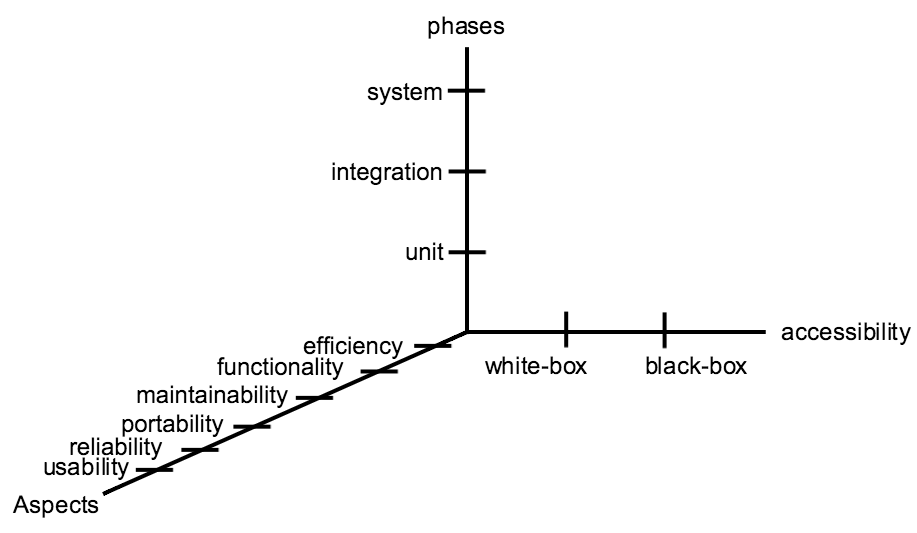
\includegraphics[width=1.0\linewidth]{figures/sorts-of-testing.png}
    \end{center}

    \caption{Sorts of testing. We can sort testing techniques by
    aspect (characteristics of quality), by phase (related to the
    target of the test), and by accessibility (related to the
    information available to construct the test cases).}
    \label{fig:sorts-of-testing}
\end{figure}

These requirements are sometimes seen as \textit{objectives} of
testing, leading to even more different testing types as listed
before. There are also different test approaches \cite{5733835}
(or perspectives) to perform testing, depending on the
information available to construct the test cases, \emph{i.e.}
accessibility:

\begin{itemize}
    \item \textbf{White-box testing:} (also known as \emph{glass box}
        \cite{5733835}) a method that tests the internal
        structure of a SUT. It is usually done at the unit level.
        This technique is also known as \emph{structural testing}
        \cite{5733835};

    \item \textbf{Black-box testing:} a method that tests the
        functionalities of a SUT without knowing its internal
        structure. The behavior of the \textit{implementation
        under test} (IUT) is only visible through a restricted
        interface called \textit{Points of Control and
        Observation} (PCOs). Such a technique is often known as
        functional testing \cite{5733835};

    \item \textbf{Grey-box testing:} the combination of white-box
        testing and black-box testing. One has access to the
        relevant parts of a SUT such as limited knowledge of the
        internal part of the SUT, and also knowledge of its
        fundamental aspects \cite{khan2012comparative}. This
        technique is sometimes called \emph{translucent testing}.
\end{itemize}

Independently of the sort of testing one choose, a common problem
in software testing is to determine a relevant and efficient set
of test cases.
\TODO{to be continued}

\subsubsection{Test selection}

Because testing cannot guarantee the absence of faults, a
challenge is to select subset of test cases from all possible
test cases with a high chance of detecting most faults. A lot of
research on \textit{test selection} (or strategies) has been
done, and there are numerous existing methods for both black-box
and white-box approaches:

\begin{itemize}
    \item \textbf{Black-box strategies:} \emph{Combinatorial
        Testing}
        (also known as \emph{Pairwise}) \cite{Tai98atest} is based on
        the observation that most faults are caused by
        interactions of at most two factors. Here we test all the
        possible discrete combinations of the parameters
        involved.  Because we cannot test all the possible input
        domain values for practical reasons, \emph{Equivalence
        Partitioning} \cite{Huang13} is a technique that divides
        the test input data into a range of values, and selects
        one input value from each range. Similarly, \emph{Boundary
        Value Analysis} \cite{Ramachandran:2003:TSC:942796.943301}
        is used to find the errors at boundaries of input domain
        rather than finding those errors in the center of input.
        We can also mention \emph{Functional Coverage} (also known as
        \emph{Inductive Testing})
        \cite{Walkinshaw:2010:IFC:1928028.1928038} where a test
        set is good enough when it achieves a given level of
        coverage;

    \item \textbf{White-box strategies:} \emph{Fuzz Testing} also known
        as \emph{Random Testing}
        \cite{Duran:1981:RRT:800078.802530,Godefroid08automatedwhitebox}
        is a method that applies random mutations to well-formed
        inputs of a program, and test the resulting values. Such
        a technique can also be applied using a black-box
        approach though, \emph{e.g.}, \cite{5387827}.
        \emph{Statistical Testing} \cite{Walton:1995:STS:210453.210458}
        is a technique where test data is generated by sampling
        from a probability distribution chosen so that each
        element of the software's structure is exercised with a
        high probability. We can also mention all techniques
        related to the code structure, such as \emph{Statement
        Testing}, \emph{Path Testing}, \emph{Branch Testing},
        \emph{Condition Testing}, \emph{Multiple Condition (MC)
        Testing}, and \emph{Loop Testing}. Another technique acts
        on the source code by mutating it, \emph{i.e.} seeding
        the implementation with a fault by applying a mutation
        operator, and then determining whether testing identifies
        this fault. This is known as \emph{Mutation Testing}
        \cite{1702444}.
\end{itemize}

The \textbf{grey-box} approach remains vague, and does not own
any proper strategy \emph{per se}. Nonetheless, the main
advantage of grey-box is to be able to combine the existing
white- and black-box strategies.

While the Industry created many different testing tools (often
originating from Academia), they mostly perform testing by hand.
Researchers in software testing have worked for decades on
automatic test generation. Automatic testing is, for instance,
one way to automate white-box approaches, but there are many
other techniques. On the contrary, Model-based Testing (MbT)
\cite{Jorgensen:1995:STC:526521} is
one research area that tries to automate black-box approaches.
In this thesis, we are interested in making production systems
more reliable by means of Model-based Testing.

\subsection{Model-based Testing}
\label{sec:related:testing:mbt}

\textit{Model-based Testing} (MbT) is application of Model-based
design for designing and optionally also executing artifacts to
perform software testing \cite{Jorgensen:1995:STC:526521}.
\emph{Models} can be used to represent the desired behavior of an
SUT, or to represent testing strategies and a test environment.
Model-based Testing can be summarized as a three-step process,
which is extended in Figure \ref{fig:mbt}:

\begin{enumerate}
    \item Formally modeling the requirements (specification).
        This is usually done by humans (\#1 in Figure
        \ref{fig:mbt}), yet feedback about the requirements can
        be obtained from the model to ease the process (\#2);

    \item Generating the test cases from the model (\#3 in Figure
        \ref{fig:mbt});

    \item Running these test cases against an actual SUT, and
        evaluating the results. The test cases provide the
        information to control (\#4 in Figure \ref{fig:mbt}) the
        implementation. The latter yields outputs that are
        observed by the test cases (\#5).  The results allow to
        issue a verdict (\#6), which provides feedback about the
        implementation (\#7). Verdicts can also provide feedback
        to either refine the model or the requirements (\#8).
\end{enumerate}

\begin{figure}[ht]
    \begin{center}
    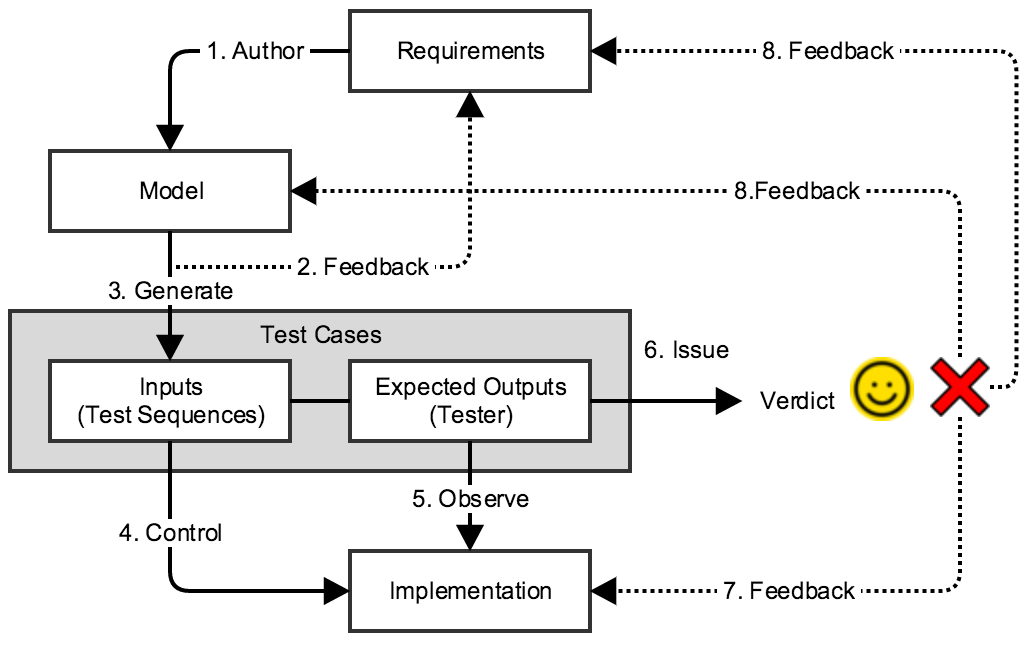
\includegraphics[width=1.0\linewidth]{figures/mbt.png}
    \end{center}

    \caption{A simplified diagram showing how MBT works. This is
    a three-step process: (i) we model the requirements (1 and
    2), (ii) we generate the test cases (3), and (iii) we run the
    test cases (4 and 5) that produce verdicts (6), which we can
    evaluate (7 and 8). Dotted arrows represent feedback, not
    "actions".}
    \label{fig:mbt}
\end{figure}

\subsubsection{What is a model?}
\label{sec:related:testing:model}

Generally speaking, a model is a representation of a "thing" that
allows for investigation of its properties, and most of the time,
a model hides the complexity of the item it represents. In the
software engineering field, models help describe software systems
in order to: (i) ease the process of studying them, (ii) leverage
them to build tools or generate documentation, or (iii) reveal
defects (validation or verification).

Such models usually describe the behaviors of the software being
modeled, and can also be known as \emph{specifications}, helping
understand and predict its behavior. In the Industry, we often
encounter a "specifications phase", as in the V-model
\cite{rook1986controlling,mathur2010advancements}, that is done
before the "coding phase". Yet, the term "specification" refers
to "a detailed formulation [...], which provides a definitive
description of a system for the purpose of developing or
validating the system" \cite{5733835}, which is a less
restrictive definition.  There are numerous models for modeling
software systems, and each describes different aspects of
software behavior. For example, control flow, data flow, and
program dependency graphs express how the implementation behaves
by representing its source code structure. It is worth mentioning
that a model does not have to completely describe it to be
effective.

We can classify models that can be employed for testing into two
categories (these lists are not exhaustive):

\begin{itemize}
    \item \textbf{Behavior/Control oriented:} \emph{Finite
        Automata} (like \emph{Finite State Machines},
        \emph{Symbolic Transition Systems}, and \emph{Labeled
        Transition Systems}) are well-known in software testing.
        They are very generic and flexible, and are a good fit
        when it comes to model software systems. For real-time
        and/or safety-critical systems, we often rely on
        synchronous languages such as \emph{Lustre}
        \cite{lustre:ieee} and \emph{SCADE}
        \cite{LeSergent:2011:SCF:2188575.2188578}. We can also
        mention \emph{Petri Nets}, \emph{Finite State Machines},
        and \emph{Timed Automata} \cite{Alur94atheory};

    \item \textbf{Data oriented (pre/post):} often using annotation
        languages originating from the \textit{Design-By-Contract}
        paradigm \cite{Meyer:1992:ADC:618974.619797}. These languages
        make it possible to express formal properties
        (invariants, pre/post-conditions) that directly annotate
        program entities (such as classes, methods, attributes)
        in the source code. Many annotation languages exist, such
        as the \emph{Java Modeling Language} (JML) \cite{jml},
        \emph{Spec\#} \cite{117852}, the \emph{Object Constraint
        Language} (OCL) \cite{Warmer:1998:OCL:291202}, the
        \emph{B-Method} \cite{Lano:1996:BLM:525749}, and
        \emph{Praspel} \cite{Enderlin:2011:PSL:2075545.2075551}.
\end{itemize}

In \cite{Sommerville:1997:REG:549198}, Sommerville and Sawyer
give some guidelines for choosing a model for software
requirements. The choice of a model depends on many factors, such
as aspects of the system under test or the testing goal.

Below we introduce a few definitions of formal models that we use
in this thesis. We mainly work with behavior-oriented models that
are finite automata since they are particularly suitable for
modeling both web applications and production systems behaviors.

\subsubsection{Model definitions}

\paragraph{Labeled Transition Systems.}
\label{sec:definitions:lts}

A \textit{Labeled Transition System} (LTS)
\cite{milner1980calculus} is a model compound of \emph{states}
with \emph{transitions}, labeled with actions, between them.  The
states model the system states and the labeled transitions model
the actions that a system can perform.  We give the definition of
the LTS model below, but we refer to \cite{ltsTretmans} for a
more detailed description.

\begin{definition}[Labeled Transition System]
    A Labeled Transition System (LTS) is a 4-tuple $<Q,L,T,q_0>$
    where:

    \begin{itemize}
    \item $Q$ is a countable, non-empty set of states;

    \item $L$ is a countable set of labels;

    \item $T \subseteq Q \times (L \cup \{\tau\}) \times Q$, with
    $\tau \not\in L$, is the transition relation;

    \item $q_0 \in Q$ is the initial state.

    \end{itemize}

    We write $q \xrightarrow[]{t} q'$ if there is a transition
    labeled $t$ from state $q$ to state $q'$ , \emph{i.e.} $(q,
    t, q') \in T$.

    The labels in $L$ represent the observable actions of a
    system, \emph{i.e.} the interactions of the system with its
    environment.
    Internal actions are denoted by the special label $\tau
    \not\in L$. Both $\tau$ and states are assumed to be
    unobservable for the environment.

	\label{def:lts}
\end{definition}

\begin{example}
    Figure \ref{fig:lts-example} presents the Labeled Transition
    System $lts_{machine}$ representing a coffee machine. There
    is a button interaction ($button$), and labels for coffee
    ($coffee$) and tea ($tea$). It is a graph where nodes
    represent states, and labeled edges represent transitions.

    We have $lts_{machine} = <\{ S1, S2, S3, S4 \}, \{ button, coffee, tea
    \}, \{ <S1, button, S2>, <S2, coffee, S3>, <S2, tea, S4> \},
    S1>$, and we can write $S1 \xrightarrow[]{button} S2$, and
    also $S1 \xrightarrow[]{button \cdot coffee} S3$, however $S1
    \not\xrightarrow[]{button \cdot tea} S3$.

    \begin{figure}[ht]
        \begin{center}
            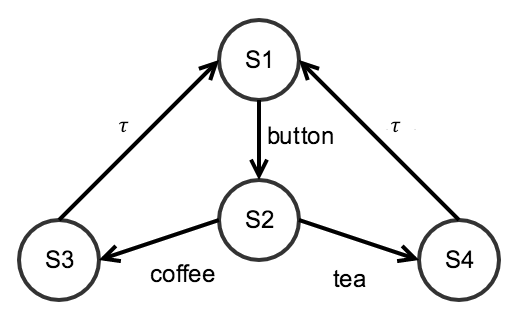
\includegraphics[width=0.7\linewidth]{figures/lts.png}
        \end{center}

        \caption{An example of a Labeled Transition System
        representing a coffee machine.}
        \label{fig:lts-example}
    \end{figure}
\end{example}

\paragraph{Symbolic Transition Systems.}
\label{sec:definitions:sts}

The \textit{Symbolic Transition System} (STS)
\cite{hennessy1995symbolic} is known as a very general and
powerful model for describing several aspects of event-based
systems. Symbolic Transition Systems (STSs) extend on LTSs by
incorporating the notion of data and data-dependent control flow.
The use of symbolic variables helps describe infinite state
machines in a finite manner. This potentially infinite behavior
is represented by the semantics of a STS, given in terms of LTS.
STS operations and transformations are often given with inference
rules. We give some definitions related to the STS model below,
but we refer to \cite{FTW05} for a more detailed description.

\begin{definition}[Symbolic Transition System]
    A Symbolic Transition System (STS) consists of
    \emph{locations} and \emph{transitions} between locations.
    Locations can be seen as symbolic states.
    A STS is defined as a tuple
    $<L,l0,V,V0,I,\Lambda,\rightarrow>$, where:

    \begin{itemize}
        \item $L$ is a countable set of locations;

        \item $l0 \in L$ is the initial location;

        \item $V$ is a finite set of location (or internal)
            variables;

        \item $V0$ is a condition on the initialization of the
            location variables $V$;

        \item $I$ is a finite set of parameters (also known as
            interaction variables), disjoint from $V$;

        \item $\Lambda$ is a finite set of symbolic actions
            $a(p)$ with $a$ a symbol, and $p=(p_1,\dots ,p_k)$ a
            finite set of parameters in $I^{k} (k \in
            \mathbb{N})$;

        \item $\rightarrow$ is a finite set of symbolic
            transitions. A symbolic transition $t =
            (l_i,l_j,a(p),G,\\A) \in \rightarrow$, from the
            location $l_i \in L$ to $l_j \in L$, also denoted by
            $l_i \xrightarrow{a(p),G,A} l_j$, is labeled by:

		\begin{itemize}
            \item An action $a(p) \in \Lambda$;

            \item A guard $G$ over $(p \cup V)$, which
            restricts the firing of the transition. Throughout
            this thesis, we often consider guards written as
            \textbf{conjunctions} of equalities: $\displaystyle
            \bigwedge_{x \in I \cup V} (x == val)$;

            \item An assignment $A$ that defines the evolution
            of the variables, $A_x$ being the function in
            $A$ defining the evolution of the variable $x \in V$.
		\end{itemize}
	\end{itemize}

	\label{def:sts}
\end{definition}

We also denote by $Proj_{x}(G)$ the projection of the guard $G$
over the variable $x \in I \cup V$, which extracts the equality
$(x==val)$ from $G$. For example, given the guard $G_1 =
[(nsys==1) \wedge (nsec==8) \wedge (point==1) \wedge (pid==1)]$,
$Proj_{nsys}(G_1) = (nsys==1)$.

For readability purpose, if $A$ is the identity function $id_V$,
we denote a transition by $l_i \xrightarrow{a(p),G} l_j$. We
also use the generalized transition relation $\Rightarrow$ to
represent STS paths: $l \xRightarrow{(a_1,G_1,A_1)\dots
(a_n,G_n,A_n)} l' =_{def} \exists l0\dots l_n, l=l0
\xrightarrow{a_1,G_1,A_1} l_1\dots
l_{n-1}\xrightarrow{a_n,G_n,A_n}l_n=l'$.

\begin{example}
    Figure \ref{fig:sts-example} presents the Symbolic Transition
    System $sts_{machine}$ representing a simple slot-machine, as
    in \cite{FTW05}. The first arrow on $L0$ indicates the
    initial location, and the fact that the machine starts with
    no money ($v = 0$). A player can insert a coin ($coin$), and
    win the jackpot in a non-deterministic manner ($v$ coins are
    passed over parameter $i$ of output action $tray$), or lose
    his money ($(i == 0)$). After that, the machine behaves as
    initially, but with a different amount of coins.

    We have $sts_{machine} = <\{L0, L1, L2, L3\}, L0, \{ v \}, \{
    v \mapsto 0 \}, \{ i \}, \{ coin, tray \}, \rightarrow >$
    where $\rightarrow$ is given by the directed edges between
    the locations in Figure \ref{fig:sts-example}.  We can write
    $L2 \xrightarrow{tray(i), G_{1} = [(i == 0)]} L0$, and
    $Proj_{i}(G_{1}) = (i == 0)$.

    \begin{figure}[ht]
        \begin{center}
            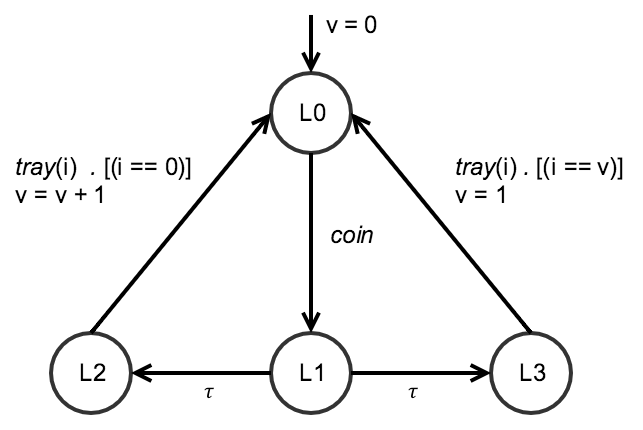
\includegraphics[width=0.7\linewidth]{figures/sts-example.png}
        \end{center}

        \caption{An example of Symbolic Transition System
        representing a simple slot-machine.}
        \label{fig:sts-example}
    \end{figure}

    \label{example:sts}
\end{example}

\begin{definition}[Variable assignment (valuation)]
    We assume that there exists a domain of values denoted by
    $D$, and a variable set $X$ taking values in $D$. The
    \emph{assignment} of variables in $Y \subseteq X$ to elements
    of $D$ is denoted by the function $\alpha: Y \rightarrow D$.
    $\alpha(x)$ denotes the assignment of the variable $x$ to a
    value in $D$.

    The empty variable assignment is denoted by $v_\emptyset$.

    We denote by $D_Y$ the set of all variable assignments over
    $Y$: $D_Y = \{ \alpha : Y \rightarrow D | v \text{ is a
    variable assignment of } Y \}$. We also denote by $id_Y$ the
    identity assignment over $Y$: $\forall x \in Y, id_Y(x)
    = x$.

    Finally, the \emph{satisfaction} of a first order formula
    \cite{huth2004logic} (\emph{i.e.} a guard) $\phi$ with
    respect to a given variable assignment $\alpha$ is denoted by
    $\alpha \models \phi$.
\end{definition}

\paragraph{Labeled Transition System semantics.}
\label{sec:definitions:lts-semantics}

A STS is associated with a Labeled Transition System to formulate
its \emph{semantics} \cite{FTW05}. A LTS semantics corresponds to
a valued state machine, without symbolic variables, which is
often infinite: the LTS states are labeled by internal variable
assignments while transitions are labeled by actions combined
with parameter assignments.

\begin{definition}[Labeled Transition System semantics]
    As defined in \cite{FTW05}, the semantics of a STS
    $\EuScript{S}=<L,l0,$ $V,$ $V0, I,\Lambda,\rightarrow>$ is
    the LTS $||\EuScript{S}||=<Q,q_0,\sum,\rightarrow>$ where:

	\begin{itemize}

        \item $Q=L \times D_V$ is a finite set of states;

        \item $q_0=(l0,V0)$ is the initial state;

        \item $\sum=\{(a(p),\alpha)  \mid  a(p)\in\Lambda, \alpha
            \in D_p\}$ is the set of \emph{valued actions};

        \item $\rightarrow$ is the transition relation $Q \times
            \Sigma \times Q$ defined by the following rule:\\
	\end{itemize}
    \begin{center}
    {\Large
    $\frac{l_1 \xrightarrow{a(p),G,A}l_2,\alpha \in D_p, v \in D_V, v'
        \in D_V, v \cup \alpha \models G, v'=A(v \cup \alpha)}{(l_1,v)
            \xrightarrow{a(p),\alpha} (l_2,v') }$
    }
	\end{center}

	\label{def:semantics}
\end{definition}

The rule above can be read as follows: for a STS transition $l_1
\xrightarrow{a(p),G,A}l_2$, we obtain a LTS transition $(l_1,v)$
$\xrightarrow{a(p),\alpha} (l_2,v')$ with $v$ a variable
assignment over the internal variable set if there exists an
assignment $\alpha$ such that the guard $G$ evaluates to true
with $v \cup \alpha$. Once the transition is executed, the
internal variables are assigned with $v'$ derived from the
assignment $A(v \cup \alpha)$.

In addition, \emph{runs} and \emph{traces}, which represent
\emph{executions} and \emph{event sequences}, can also be derived
from LTS semantics:

\begin{definition}[Runs and traces]
    Given a STS $\EuScript{S}=$ $<L,l0,V,V0,I,\Lambda,
    \rightarrow>$, interpreted by its LTS semantics
    $||\EuScript{S}||=<Q,q_0,\sum,\rightarrow>$, a run $q_0 \cdot
    \alpha_0 \cdot \dots \cdot \alpha_{n-1} \cdot q_n$ is an
    alternate finite sequence of states and valued actions,
    concatenated with the $\cdot$ operator.
    $Run(\EuScript{S})=Run(||\EuScript{S}||)$ is the set of runs
    found in $||\EuScript{S}||$.

    It follows that a trace of a run $r$ is defined as the
    projection $proj_{\sum}(r)$ on the actions.

    \label{def:runs-and-traces}
\end{definition}

\paragraph{Input/Output Symbolic Transition Systems.}
\label{sec:definitions:iosts}

An Input/Output Symbolic Transition System (IOSTS)
\cite{Rusu:2000:AST:647982.743536} is a STS where the action set
is divided into two subsets: one containing the inputs, beginning
with $?$, to express actions expected by the system, and another
containing outputs, beginning with $!$, to express actions
produced by the system. When no output action is possible, the
only observation that can be made is \emph{quiescence}
\cite{Tre96}.

\begin{definition}[Input/Output Symbolic Transition System]
    As defined in \cite{Rusu:2000:AST:647982.743536}, an
    Input/Output Symbolic Transition System (IOSTS)
    $\EuScript{S}$ is a tuple $<L,l0,V,V0,I,\Lambda,\rightarrow>$, where:

\begin{itemize}
    \item $L$ is a finite set of locations;

    \item $l0 \in L$ the initial location;

    \item $V$ is a finite set of location (or internal)
        variables;

    \item $V0$ is a condition on the initialization of the
        location variables $V$;

    \item $I$ is a finite set of parameters, disjoint from $V$;

    \item $\Lambda$ is a finite set of symbolic actions $a(p)$,
        with $a$ a symbol, and $p = (p_1,\dots,p_k)$ a finite set
        of parameters in $I^k(k \in \mathbb{N})$. $p$ is assumed
        unique. $\Lambda$ is partitioned into a set of input
        actions $\Lambda^I$ and a set of output actions
        $\Lambda^O$, and we write $\Lambda = \Lambda^I \cup
        \Lambda^O \cup \{!\delta \}$: $\Lambda^I$, with $\delta$
        the quiescence;

    \item $\rightarrow$ is a finite set of symbolic transitions.
        A symbolic transition $(l_i,l_j,a(p),G,A)$, from the
        location $l_i \in L$ to $l_j \in L$, also denoted by $l_i
        \xrightarrow{a(p),G,A} l_j$, is labeled by:

        \begin{itemize}
            \item A action $a(p) \in \Lambda$;

            \item A guard  $G$ over $(p \cup V \cup T(p \cup
                V))$, which restricts the firing of the
                transition. $T(p \cup V)$ is a set of functions
                that return boolean values only (also known as
                predicates) over $p \cup V$;

            \item An assignment $A$ that defines the evolution of
                the variables. $A$ is of the form $(x:=A_x)_{x\in
                V}$, where $A_x$ is an expression over $V \cup p
                \cup T(p \cup V)$.
        \end{itemize}
\end{itemize}
\end{definition}

\begin{example}
    Figure \ref{fig:iosts-example} is the IOSTS of the
    slot-machine introduced in Example \vref{example:sts}.  We
    have $iosts_{machine} = <\{L0, L1, L2, L3\}, L0, \{ v \}, \{
    v \mapsto 0 \}, \{ i \}, \{ coin?, tray! \}, \rightarrow >$
    with $\Lambda^I = \{ coin? \}$ and $\Lambda^O = \{ tray! \}$.

    \begin{figure}[ht]
        \begin{center}
            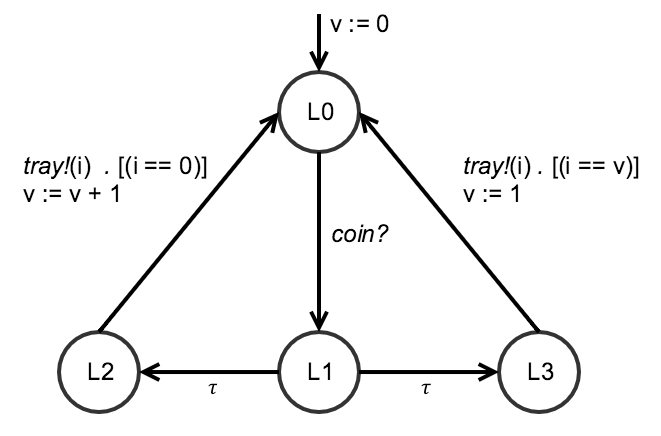
\includegraphics[width=0.7\linewidth]{figures/iosts-example.png}
        \end{center}

        \caption{An example of Input/Output Symbolic Transition
        System representing a simple slot-machine.}
        \label{fig:iosts-example}
    \end{figure}
\end{example}

In this thesis, we chose to use these models to represent the
behaviors of web applications and production systems in order to
perform Model-based Testing, \emph{i.e.} relying on models to
perform testing, mainly to prevent regressions. \emph{Conformance
Testing} is a black-box testing method leveraging formal methods
\cite{tretmans1992formal}. We give a few definitions related to
Conformance Testing below.

\subsubsection{Conformance Testing}

In this section, we introduce a few common terms defining what
\emph{Conformance Testing}
\cite{brinksma1989formal,tretmans1992formal,Tretmans:1993:FAC:648128.747730}
is, and how it works in general.

\paragraph{Test hypothesis.} Executing a test case on a system
yields a set of observations. Every observation represents a
part of the \textit{implementation model} of the system. The set
of all observations made with all possible test cases represents
the complete implementation model of the system. The \emph{test
hypothesis} \cite{Bernot:1991:TAF:112287.112303} is that, for
every system, there is a corresponding observational equivalent
implementation model: $\forall \text{ } iut \in IMPS, \exists
\text{ } I_{iut} \in MODS$, where $iut$ is a concrete
\emph{implementation under test}, $IMPS$ is the universe of
implementations, $I_{iut}$ is a model of $iut$, and $MODS$ is the
universe of the models of all \emph{implementations under test}.

\paragraph{Conformance.} To check whether an implementation under
test $iut$ conforms to a specification $spec$, we need to know
precisely what it means for $iut$ to conforms to $spec$,
\emph{i.e.} a formal definition of conformance is required
\cite{ltsTretmans}. As $iut$ is a real, physical "thing", which
consists of software (and sometimes physical devices), we cannot
use it as a formal object. We rely on the test hypothesis
mentioned previously to reason about implementations under test
as if they were formal implementations. By doing this, we can
define conformance with a formal relation between models of
implementations and specifications, \emph{i.e.} an
\emph{implementation relation}.

\paragraph{Implementation relation.} To formally define
conformance between an implementation under test $iut$ and a
specification $spec$, we use the notion of an
\emph{implementation relation}: $imp \subseteq MODS \times
SPECS$, with $SPECS$ the set of specifications. We can find
different implementation relations, \emph{e.g.},
\cite{Bri88,phalippou94}.

An implementation $iut$ \textbf{conforms to} a specification
$spec$ if the existing model $I_{iut}$ of $iut$ is
\textit{imp-related} to $spec$: $I_{iut} \textbf{imp} spec$.
There are many conformance relations in the literature, which we
can organize in three categories:

\begin{itemize}
    \item \textbf{Equivalence relations:} \emph{Isomorphism},
        \emph{Bisimulation}
        \cite{Abdulla06,Fernandez89animplementation}, \emph{Trace
        Equivalence}, \emph{Testing Equivalence}
        \cite{Abramsky1987225}, \emph{Refusal Equivalence}
        \cite{Phillips86};

    \item \textbf{Preorder relations:} \emph{Observation
        Preorder}, \emph{Trace Preorder} \cite{DNH84},
        \emph{Testing Preorder} \cite{Beohar2015}, \emph{Refusal
        Preorder};

    \item \textbf{Input-Output relations:} \emph{Input-Output
        Testing}, \emph{Input-Output Refusal}, \emph{ioconf}
        \cite{tretmans1996conformance}, \emph{ioco} \cite{Tre96}.
\end{itemize}

\paragraph{Conformance testing.} Conformance Testing
assesses conformance to an unknown implementation under test
$iut$ to its specification $spec$ by means of test experiments.
Experiments consist of stimulating $iut$ in certain ways and
observing its reactions. This process is called \textit{test
execution}, which is defined below.

\paragraph{Test execution.} The successful execution of a test
case $TC$ can be written as follows: $I_{iut} \text{ }
\mathbf{passes} \text{ } TC$. We extend it to a test
suite $TS$: $I_{iut} \text{ } \mathbf{passes} \text{ } TS
\Leftrightarrow \forall \text{ } TC \in TS : I_{iut} \text{ }
\mathbf{passes} \text{ } TC$. On the contrary, $I_{iut} \text{ }
\mathbf{fails} \text{ } TC \Leftrightarrow I_{iut} \text{ } \neg
\mathbf{passes} \text{ } TC$.

This leads to three properties on the test suite $TS$
\cite{ltsTretmans}:

\begin{itemize}
\item \textbf{Soundness:} $\forall \text{ } iut \in IMPS, iut$
conforms to $spec \implies iut \text{ } \mathbf{passes} \text{ }
TS$;

\item \textbf{Exhaustiveness:} $\forall \text{ } iut \in IMPS,
iut \text{ } \mathbf{passes} \text{ } TS \implies iut$ conforms
to $spec$;

\item \textbf{Completeness:} $\forall \text{ } iut \in IMPS, iut$
conforms to $spec \Leftrightarrow iut \text{ } \mathbf{passes}
\text{ } TS$.
\end{itemize}

We rely on a \textit{test architecture}, \emph{i.e.} an abstract
description of the \textit{environment} in which an
implementation under test $iut$ is embedded, and where it
communicates with a \textit{tester}.

\paragraph{Tester and verdicts.} A tester executes the test
cases. To be able to decide about the success of each, a
\textit{verdict} (most of the time, $pass$ or $fail$) is attached
to each state of each test case.

Neither Model-based Testing nor Conformance Testing state that
"executing the test cases" implies to interact with the system
under test. Indeed, there is a last perspective related to
whether the testing method stimulates the system or not.

\subsection{(Active and) passive testing}
\label{sec:related:testing:active-passive}

In this section, we introduce two different approaches based on
how we apply the test cases to the system under test:

\begin{itemize}
    \item \textbf{Active testing}, which is the classical process
        in which a tester examines the functionality of a unit
        under test before that unit is being deployed, \emph{i.e.}
        during its development;

    \item \textbf{Passive testing}, which takes place after the
        deployment of that unit, and requires, for instance, the
        presence of a \textit{monitor}. Passive testing is also
        useful when one wants to test a system during a long
        period of time.
\end{itemize}

While active testing can take place as black-, grey-, or white-box
testing, passive testing is often a special form of black-box
testing. Active testing works by stimulating the system under
test, \emph{i.e.} observing outputs of an implementation for predefined
inputs. Most of the classical testing techniques and tools found
in the Industry perform active testing, \emph{e.g.}, \textit{xUnit}
frameworks
\footnote{\url{http://www.martinfowler.com/bliki/Xunit.html}}.

Passive testing rather examines the input/output behavior of an
implementation without preordaining the input. One advantage of
passive testing is that it does not disturb the system, and it
can be applied to large (distributed) systems. While most of the
works on passive testing are related to networks, protocols, and
web services, such a technique can be particularly suitable for
production systems such as Michelin's systems.

Several works, dealing with passive testing of protocols or
components, have been proposed over the last decade. For all of
these, the tester is made up of a module, located in the
implementation environment, which collects trace sets. These
works can be grouped in three different categories:

\begin{itemize}

    \item \textbf{Invariant satisfiability:} invariants represent
        properties that are always true. They are constructed by
        hand from a specification, and later checked on the
        collected traces. Similarly to runtime verification
        \cite{Leucker2009293}, this approach allows to test
        complex properties on an implementation. It gave birth to
        several works in the literature. For instance, the
        passive testing method, presented in \cite{CMdO09}, aims
        to test the satisfiability of invariants on Mobile ad hoc
        network (MANET) routing protocols.  Different steps are
        required: definition of invariants from the
        specification, extraction of execution traces with
        sniffers, verification of the invariants on the trace
        set. Other works focus on \emph{Component-based System
        Testing}: in this case, passive methods are usually used
        to check conformance or security. For instance, the
        \textit{TIPS} tool \cite{5552735} performs an automated
        analysis of the captured trace sets to determine if a
        given set of timed extended invariants are satisfied. As
        in \cite{CMdO09}, invariants are constructed from the
        specification and traces are collected with network
        sniffers. Cavalli \emph{et al.} propose an approach for
        testing the security of web service compositions in
        \cite{cavalli2009passive}. Security rules are here
        modeled with the Nomad language \cite{cuppens2005nomad},
        which expresses authorizations or prohibitions by means
        of time constraints. Preliminary, a rule set is manually
        constructed from a specification. Traces of the
        implementation are extracted with modules that are placed
        at each workflow engine layer that executes web services.
        Then, the method checks, with the collected traces, that
        the implementation does not contradict security rules.
        Andrés \emph{et al.} presented a methodology to perform
        passive testing of timed systems in
        \cite{andres2012formal}. The paper gives two algorithms
        to decide the correctness of proposed invariants with
        respect to a given specification and algorithms to check
        the correctness of a log, recorded from the
        implementation under test, with respect to an invariant;

    \item \textbf{Forward checking:} implementation reactions are
        given on-the-fly to an algorithm that detects incorrect
        behaviors by covering the specification transitions with
        these reactions. Lee \emph{et al.} proposed a passive
        testing method dedicated to wired protocols
        \cite{1621118}.  Protocols are modeled with
        \textit{Event-driven Extended Finite State Machines}
        (EEFSM), compound of variables.  Several algorithms on
        the EEFSM model and their applications to the Open
        Shortest Path First (OSPF) protocol and Transmission
        Control Protocol (TCP) state machines are presented.
        Algorithms check whether partial traces, composed of
        actions and parameters, meet a given symbolic
        specification on-the-fly. The analysis of the symbolic
        specification is performed by means of configuration. A
        configuration represents a tuple gathering the current
        state label, and a set of assignments and guards modeling
        the variable state;

    \item \textbf{Backward checking:} Alcalde \emph{et al.}
        proposed an approach that processes a partial trace
        backward to narrow down the possible specifications in
        \cite{alcalde2004network}. The algorithm performs two
        steps. It first follows a given trace backward, from the
        current configuration to a set of starting ones,
        according to the specification. With this step, the
        algorithm finds the possible starting configurations of
        the trace, which lead to the current configuration. Then,
        it analyses the past of this set of starting
        configurations, also in a backward manner, seeking for
        configurations in which the variables are determined.
        When such configurations are reached, a decision is taken
        on the validity of the studied paths (traces are
        completed). Such an approach is usually applied as a
        complement to forward checking to detect more errors.
\end{itemize}

It is worth mentioning that passive testing has also been
successfully applied for fault management \cite{965909}, fault
detection \cite{Ural:2007:IAP:1270230.1270259}, and security
purpose \cite{4698175}. To summarize, while passive testing is
less powerful than active testing, because the latter allows a
closer control of the implementation under test, passive testing
still presents interesting advantages:

\begin{itemize}
    \item Passive testing is less costly than active testing in
        general since it does not have to control the
        implementation under test;

    \item Passive testing can be applied to large systems where
        active testing is not even feasible, such as systems with
        many different components, \emph{e.g.}, software oriented
        architectures, distributed systems, but also production
        systems such as the ones we target in this thesis.
\end{itemize}

\section{Model inference}
\label{sec:related:modelinf}

In the Industry, software models as defined in
\crossref{sec:related:testing}{sec:related:testing:model} are
often neglected: specifications are not up to date (or even
missing), models are neither accurate nor sound, and also rarely
formals.

Such a situation can be comprehensible because writing complete
documentation and especially formal models is often a tedious and
error prone task. That is why lightweight and incomplete models
are usually found in the Industry. This leads to several issues,
e.g., the toughness of testing applications with a good test
coverage, the difficulty to diagnose failures, or to maintain
models up to date since they are poorly documented.

Solutions to these problems can be initiated by means of model
inference. This research domain originates from works on language
learning started in the 1960s with Gold \cite{Gold1978302}, based
on previous work to formalize natural languages. Model inference
here describes a set of methods that infer a specification by
gathering and analyzing system executions and concisely
summarizing the frequent interaction patterns as state machines
that capture the system's behavior. These models, even if
partial, can be examined by a developer, to refine the
specification, to identify errors, and can be very helpful for
in-depth analysis, etc. Models can be generated from different
kinds of data samples such as affirmative and negative answers
\cite{Angluin198787}, execution traces
\cite{Krka:2010:UDE:1810295.1810324}, documentation
\cite{ZhongZXM11}, source code
\cite{Salah05scenariographer,Pradel:2009}, network traces
\cite{6079839} or from more abstract documentation such as Web
Service Description Language (WSDL)
description \cite{Bertolino:2009:ASB:1595696.1595719}.  Model
inference is employed for different purposes. One can infer
models from log files in order to retrieve important information
in order to identify failure causes \cite{4700316}. It has also
successfully been applied to intrusion detection \cite{debar00},
searching for features in execution traces that allow to
distinguish browsers from other software systems. A prominent use
of model inference also concerns Model-based Testing
\cite{Lorenzoli2008,tap2011,MobiGUITARIEEESoftware2014} and
verification \cite{Ammons:2002:MS:565816.503275}.

In the literature, we can find different techniques to infer
models that can be organized in two main categories. In the first
category, we find the techniques that interact with systems or
humans to extract knowledge that is then studied to build models.
We refer to these methods as active methods. Other works infer
models by assuming that system samples, e.g., a set of traces, is
provided for learning models. We refer to this principle as
passive methods since no interaction is required.

In the following section, we give an overview of prominent active
inference approaches: we introduce $\EuScript{L}^*$-based
techniques in Section \ref{sec:active-letoile}, incremental
learning techniques in Section \ref{sec:active-increment}, and
the model generation by means of automatic testing of
event-driven applications providing Graphical User Interfaces
GUIs) in Section \ref{sec:active-crawling}. Passive inference
techniques are extensively described in Section
\ref{sec:passive}. We cover passive inference techniques using
event sequence-based abstraction in Section
\ref{sec:passive-fsa}, using state-based abstraction in Section
\ref{sec:passive-spec}. Then, we present some white-box
approaches in Section \ref{sec:passive-white}, and we also
mention a few techniques that leverage documentation to infer
models in Section \ref{sec:passive-others}.

%%%%%%%%%%%%%%%%%%%%%%%%%%%%%%%%%%%%%%%%%%%%%%%%%%%%%%%%%%%%%%%%%

\subsection{Active model inference}
\label{sec:active}

\begin{figure}[h]
    \begin{center}
        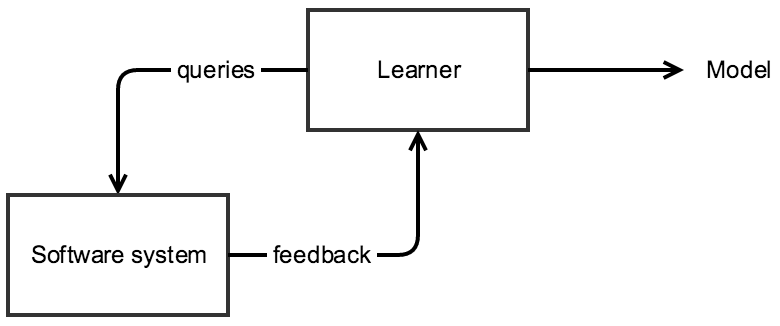
\includegraphics[width=0.9\linewidth]{figures/active.png}
    \end{center}

    \caption{Active model inference principle. Interactions are
        performed with queries that produce feedback a learner
        can use to build a model.}
    \label{fig:active}
\end{figure}

Active inference refers to algorithms that actively interact with
black-box systems or people to extract knowledge about a
(software) system, which is then expressed in a model.
Interactions are performed with kinds of queries, which are
sometimes replaced by testing techniques. A model generator or
learner then uses this feedback to incrementally build several
models, or to refine the model under generation. Many existing
active inference techniques have been initially conceived upon
two concepts: the $\EuScript{L}^*$ algorithm, presented in
Section \ref{sec:active-letoile}, and incremental learning,
presented in Section \ref{sec:active-increment}. Several more
recent papers also proposed crawling techniques of Graphical User
Interface (GUI) applications, i.e. exploring them through their
GUIs with automatic testing. We introduce some of them in Section
\ref{sec:active-crawling}.

\subsubsection{$\EuScript{L}^*$-based techniques and related}
\label{sec:active-letoile}

\begin{figure}[h]
    \begin{center}
        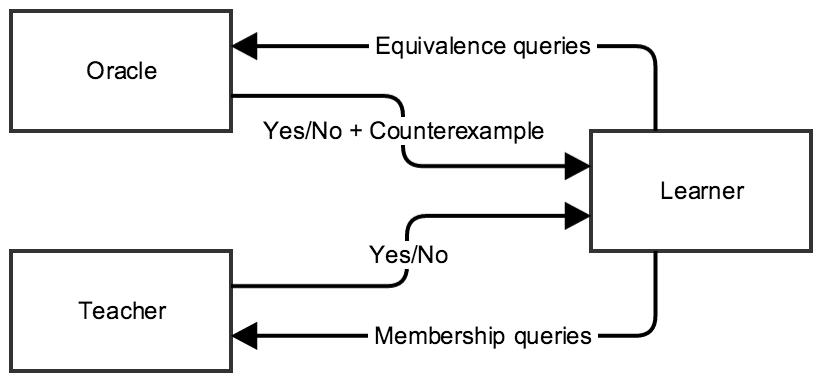
\includegraphics[width=0.9\linewidth]{figures/angluin.png}
    \end{center}

    \caption{The principle of $\EuScript{L}^*$-based learning
    algorithms with two kinds of queries: membership queries and
    equivalence queries.}
    \label{fig:angluin}
\end{figure}

The $\EuScript{L}^*$ algorithm by Angluin \cite{Angluin198787} is
one of the most widely used active learning algorithm for
learning \textit{Deterministic Finite Automata} (DFA). The
algorithm has indeed been applied to various problem domains,
e.g., protocol inference or the testing of circuits. It is
designed to learn a regular language $\EuScript{L}$ by inferring
a minimal DFA $\EuScript{A}$ such that
$\EuScript{L}(\EuScript{A})=\EuScript{L}$, with
$\EuScript{L}(\EuScript{A})$ the set of strings of $\EuScript{A}$
leading to one of its states from its initial one. The algorithm,
also known as the \textit{learner}, knows nothing about
$\EuScript{A}$ except its input alphabet. It relies on two roles,
a \textit{teacher}, who may answer whether a given string is in
the language, and an \textit{oracle}, answering whether the
current DFA proposed by the learner is correct or not. The
learner interacts with the teacher and the oracle by asking them
two kinds of queries, as depicted in Figure \ref{fig:angluin}:

\begin{itemize}
    \item A \textbf{membership query}, consisting in asking the
        teacher whether a word is contained in the regular
        language.  If the word is accepted, it is considered as a
        \textit{positive} example, otherwise it represents a
        negative example;

    \item An \textbf{equivalence query}, consisting in asking the
        oracle whether an hypothesized DFA $\EuScript{M}$ is
        correct, i.e. $\EuScript{L}(\EuScript{M}) =
        \EuScript{L}(\EuScript{A})$. If the oracle answers $no$,
        it provides a counterexample.
\end{itemize}

By taking counterexamples into account, the $\EuScript{L}^*$
algorithm iterates by asking new queries and constructing a new
hypothesized DFA $\EuScript{M}$, until it gets an automaton that
is equivalent to the black-box. The $\EuScript{L}^*$ algorithm
uses an observation table to classify the strings given in
membership queries as members or non-members of the unknown
regular language. In an observation table, the rows are fulfilled
by prefix-closed strings, the columns are labeled by
suffix-closed strings. The algorithm gradually fills the entry
$(u,v)$ for row $u$ and column $v$ by a boolean value after
receiving a reply for a membership query for $uv$. Once the
oracle answers $yes$, the minimal DFA for the language is derived
from this observation table. The $\EuScript{L}^*$
algorithm has also be applied on Mealy machines as shown in
\cite{DBLP:phd/de/Niese2003,steffen11}. With Mealy machines, the
event set is segmented into inputs and outputs. The rows of the
table are filled with prefix-closed input sequences. The columns
of the table are labeled with input suffix sequences, which
represent the distinguishing sequences of the states of the
upcoming Mealy machine. The table cells are completed by the last
outputs given by the teacher after receiving the concatenations
of prefixes and suffixes.

In domains such as model inference where strings and answers
usually don't come from human experts but from experiments,
active learning with query synthesis is considered a promising
direction \cite{settles.tr09}. Nevertheless, this method has the
disadvantages of requiring a lot of iterations and an heavy use
of an expert oracle. Several papers focused on these issues by
revisiting, optimizing and/or upgrading $\EuScript{L}^*$, others
proposed to apply it in specific application contexts, as
summarized below.

Raffelt et al. introduced \textit{LearnLib}
\cite{Raffelt:2005:LLA:1081180.1081189}, a library for learning
both DFA and Mealy machines. It implements the $\EuScript{L}^*$
\cite{Angluin198787} learning algorithm, which is optimized with
\textit{approximate equivalence queries}. Furthermore, the
notion of teacher is replaced with conformance testing
techniques. The query optimization is mainly based on
\textit{filters}, which are specific properties of reactive
systems that help in the removal of useless queries. A query
whose response can be deduce from the previous ones is also
ignored. Additionally, statistical data acquisition can be
employed to evaluate the learning procedure. These features make
\textit{LearnLib} a powerful tool if a teacher is available.
Later, Merten et al. revisited \textit{LearnLib} in a tool called
\textit{Next Generation LearnLib} (NGLL) \cite{ngll11}, a machine
learning framework providing infrastructure for practical
application, including the tool \textit{LearnLib Studio}, a
graphical interface for designing and executing learning and
experimentation setups, plus a set of Java libraries. Howar et
al. pursued the inference of models  and proposed a technique and
an implementation on top of \textit{LearnLib} to actively learn
register automata in \cite{howarRA2012}. Register automata, also
known as \textit{Finite Memory Automata} \cite{Kaminski1994329},
are models that are capable of expressing the influence of data
on control flows. The algorithm directly infers the effect of
data values on control flows as part of the learning process. As
a consequence, the models are more expressive than Finite State
Machines (FSM) and the implementation also  outperforms the
classic $\EuScript{L}^*$ algorithm. Howar et al. optimized this
approach and proposed a method to infer \textit{semantic
interfaces} of data structures on the basis of active learning
and systematic testing in \cite{howar2012}. Semantic interfaces
transparently reflect the behavioral influence of parameters at
the interface level.  They defined \textit{Register Mealy
Machines} (RMMs) to express the data structures behavior
concisely, but also because RMMs can be learned much more
efficiently than both \textit{Register Automata} and plain Mealy
machines.

Berg et al. also revisited the $\EuScript{L}^*$ algorithm in
\cite{regularinfBerg06} to infer parameterized systems, which are
kinds of automata composed of parameters and guards over
parameters (boolean expressions) labeled on transitions. The
approach completes the  $\EuScript{L}^*$ algorithm with guard
inference. This algorithm is intended to infer parameterized
systems where guards of transitions use only a small subset of
all parameters of a particular action type. Such a work has been
used later to infer state machines for systems with parameterized
inputs \cite{regularinfBerg08}. Here, behavioral models are
inferred (finite-state Mealy machine) for finite data domains,
and then, models are abstracted to symbolic Mealy machines,
encoding extrapolated invariants on data parameters as guarded
transitions.

Other work proposed to optimize the $\EuScript{L}^*$ algorithm
itself. For instance, Irfan et al. proposed the $\EuScript{L}_1$
algorithm \cite{irfan12} to infer Mealy machines, which uses a
modified observation table and avoids adding unnecessary elements
to its columns and rows. In short, the algorithm only keeps the
distinguishing input sequences and their suffixes in the columns
of the observation table, and the access sequences, i.e. the
input sequences allowing to reach a state, in the rows. These
improvements reduce the table size and the worst case time
complexity.

A common problem to the algorithms presented above is the time
spent querying the oracle or the teacher, and several
competitions, e.g., the ZULU challenge \cite{zulu} have been
proposed to optimize the learning task by trying to make easier
queries, or queries for which the oracle's answer is simpler.
Concretely, the purpose of such competitions is to optimize the
learning algorithm with heuristics to reduce the number of
equivalence and membership queries. But having an oracle knowing
all about the target model is a strong assumption. Hence, other
works propose a completely different solution called incremental
learning.

\subsubsection{Incremental learning}
\label{sec:active-increment}

Instead of querying teachers and oracles to check whether strings
and models are correct, incremental learning techniques assumes
receiving successively positive or negative samples, also called
observations. Several models are incrementally built in such a
way that if a new observation $\alpha$ is not consistent with the
current model, the latter is modified such that $\alpha$ becomes
consistent with the resulting new model.  In general, a learning
algorithm is said incremental if: (i) it constructs a sequence of
hypothesis automata $H_0, \dots, H_n$ from a sequence of
observations $o_0, \dots, o_n$  about an unknown automaton $A$,
and (ii) the construction of hypothesis $H_i$ can reuse aspects
of the construction of the previous hypothesis $H_{i-1}$.

Dupont proposed an incremental extension of the Regular Positive
and Negative Inference (RPNI) algorithm, called \textit{Regular
Positive and Negative Incremental Inference} (RPNI2)
\cite{Dupont96incrementalregular}. In short, RPNI requires
positive and negative samples as a whole and builds DFAs. It
merges the blocks of states having the same prefixes (words
accepted from a state leading to all the other states) and such
that the prefixes augmented by one symbol are not in the negative
samples. The inference process of the RPNI algorithm can be seen
as a passive approach that is not incremental since it has to
be restarted from scratch when new learning data are available.
The RPNI2 algorithm overcomes this limitation by dealing with
sequential presentation, i.e. the learning data are presented one
at a time in a random order.

Parekh et al. \cite{parekh98} proposed an incremental extension
of Angluin's \textit{ID} algorithm \cite{ANGLUIN198176}, the
latter being not incremental since only a single model is
ever produced. This extension called \textit{Incremental ID}
(IID) constructs DFAs from observation sets. Membership queries
are sent to an oracle to check whether the current DFA is
correct. IID is guaranteed to converge to the target DFA, and has
polynomial time and space complexities. Sindhu et al. also
enhanced the ID algorithm by proposing another incremental
version called \textit{Incremental Distinguishing Sequences}
(IDS) \cite{journals/corr/abs-1206-2691}. The state merging is
here performed by generating the distinguishing sequence set $DS$
of every state and by refining blocks of states such that two
blocks of states are distinct if and only if they do not have the
same $DS$ sets. IDS also has polynomial time and space
complexities. In contrast with IID, the IDS algorithm solves some
technical errors and its proof of correctness is much simpler.

Meinke introduced the \textit{Congruence Generator Extension}
(CGE) algorithm in \cite{meinkeCGE} to infer Mealy automata by
applying the term rewriting theory and a congruence generator.
Here congruence is an equivalence relation on states and on
outputs. Meinke describes this algorithm as being both sequential
and incremental. First, it produces a sequence of hypothesis
automata $\EuScript{A}_0, \dots, \EuScript{A}_n$, which are
approximations to an unknown automaton $\EuScript{A}$, based on
sequence of information (queries and results) about
$\EuScript{A}$. CGE is incremental because the computation
of a new hypothesis automaton $\EuScript{A}_i$ is based upon the
previous $\EuScript{A}_{i-1}$. Meinke shows here that using
finitely generated congruences increases the efficiency of
hypothesis automaton representation, which are deterministic
and can be directly analyzed (e.g, for verification purpose). CGE
has some features in common with the RPNII algorithm mentioned
previously: both RPNII and CGE perform a recursive depth-first
search of a lexicographically ordered state set with
backtracking. Nevertheless, RPNII is designed for Moore machines
while CGE is designed for Mealy machines. RPNII represents the
hypothesis automaton state set by computing an equivalence
relation on input strings whereas CGE relies on finite congruence
generator sets represented as string rewriting systems that are
used to compute normal forms of states.

Some incremental learning algorithms have been associated with
testing techniques to detect bugs without having an initial
specification. In \cite{Meinke:2004:ABT:1007512.1007532,tap2011},
this concept is called \textit{Learning-Based Testing}. It aims
at automatically generating the test cases by combining
model-checking with model inference. For example, Meinke and
Sindhu \cite{tap2011} introduced an incremental learning
algorithm named \textit{Incremental Kripke Learning} (IKL) for
Kripke structures modeling reactive systems. Here, the test
cases are generated and executed to extract observations.
Afterwards, models are derived from these observations with an
incremental learning algorithm, and model-checking is applied on
the inferred models to check if initial requirements are met. If
not, counterexamples are collected, and the test cases are
generated from them.

Combining incremental model inference with testing has also been
studied with applications providing Graphical User Interfaces
(GUIs), which are event-driven. We present some works related to
the model inference of GUI applications in the next section.

\subsubsection{Model inference of GUI applications}
\label{sec:active-crawling}

\begin{figure}[ht]
    \begin{center}
        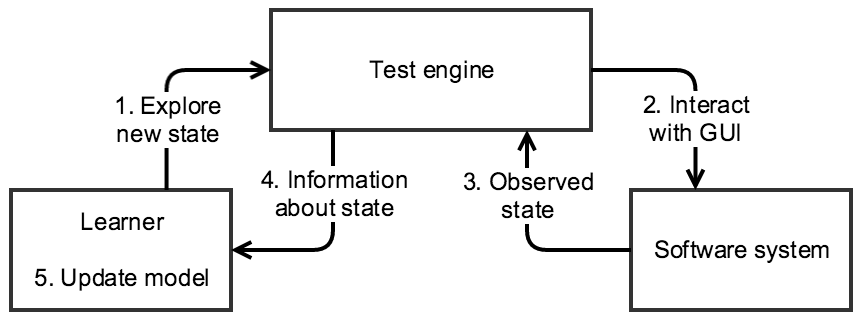
\includegraphics[width=0.9\linewidth]{figures/crawler.png}
    \end{center}

    \caption{The principle of inferring models with crawling
    techniques. The learner asks a test engine to stimulate the
	software under test through its GUI, and constructs a model
	using the information gathered by the test engine.}
    \label{fig:crawler}
\end{figure}

The works presented in this section originate from the automatic
testing of GUI applications, e.g., desktop, web, and more recently
mobile applications. As depicted in Figure \ref{fig:crawler},
models are generated by a learner that updates the model under
generation using events and states given by an automatic test
engine. This test engine stimulates the application through its
GUI (by triggering events, e.g., clicking on a button or a link),
and collects all the observed screens.  Screen after screen, the
application is explored (the technical term is: crawled) until
there is no more new screen to explore or until some conditions
(e.g., based on the processing time or the code coverage rate)
are satisfied. The collected events and screens are often
represented with transitions and states in a graph or state
machine, which expresses the functional behavior of the
application observed from its GUI. As the number of screens may
be infinite, some approaches require state abstractions to limit
the model size, and a few others merge equivalence states (the
equivalence relation being defined with regards to the context of
the application).

\begin{table}
	\begin{tabular}{| c | c | c | c | c | c | c |}

		\hline

		Paper &2& 3 & 4& 5 & 6 & 7 	\\
		\hline

		%\cite{monkey}                           &mobile                 &B  &  &IM &Random   & Yes	\\

		\cite{hungar2002}                       &distributed
        systems   &B  &  &FM&$\EuScript{L}^*$       & \\

		%\cite{Memon:2003}                        &desktop                &B  &  &M &DFS      &  \\

		\cite{5416728}                          &web                    &B  &  &  &Concolic & Yes \\

		\cite{concolicandroid12}                &mobile                 &W  &  &  &Concolic & 					\\

		\cite{Joorabchi:2012:REI:2420240.2420457}                    &mobile                 &B  &  &IM &DFS		& Yes 			 		\\

		\cite{webmate12}                        &web                    &B  &  &IM &         & Yes \\

		%\cite{dynodroid}                        &mobile                 &B  &Yes &  &Random 	& Yes		\\

		\cite{5954416,Amalfitano:2012:UGR:2351676.2351717}     &mobile                 &B  &  &IM &BFS DFS 	& Yes	\\

		\cite{guitar,MobiGUITARIEEESoftware2014}          &desktop, mobile        &B	&  &FM &DFS		& Yes  \\

		\cite{crawljax:tweb12}                  &web                    &B	&  &FM&Multiple &	\\

		\cite{4656395}                          &web                    &B 	&  &IM &DFS 		&   \\

		\cite{Choi2013}                         &mobile                 &B  &  &FM&DFS      &   \\

		\cite{WPX13}                            &mobile                 &G  &  &IM &Multiple(2)		& 	\\

		\cite{Azim13}                           &mobile                 &G	&Yes &IM &DFS		& Yes \\

		\cite{SP15}								&mobile                 &B	&Yes &FM &Multiple		& Yes \\
		\hline
	\end{tabular}
	\\

	\caption{An overview of some works on GUI application
	crawling. Column 2 represents the type of application under
	analysis. Column 3 indicated the accessibility (black-box
	(B), white-box (W), grey-box (G)). Column 4 gives whether the
	technique requires an external environment. Column 5
	indicates whether the technique builds formal models (FM) or
	non-formal models (IM). Column 6 gives the strategy or
	algorithm used to crawl the application. Last column (7)
	shows whether the technique handles potential crashes, i.e.
	errors encountered during crawling.}
	\label{table:gui_works}
\end{table}

All these approaches focus on different applications seen in
different viewpoints. We chose to summarize them in Table
\ref{table:gui_works}, considering the following features:

\begin{itemize}
	\item \textbf{Type of application and accessibility (col.
	2 and 3):} most of the approaches focus on desktop, web, or
	mobile applications. These applications share some common
	features, e.g., the events that can be applied on screens.
	Some papers focus on other kinds of systems though, e.g.,
	distributed and legacy systems \cite{hungar2002}.

	The accessibility refers to the information available and
	considered by a technique. Applications are often seen as
	black-boxes even though some authors prefer to consider
	white- or grey-boxes Column 3 in Table
	\ref{table:gui_works} indicates the accessibility chosen
	for each technique. For instance,
	\cite{concolicandroid12,5416728} present testing frameworks
	that exercise mobile applications and rely upon a
	systematic test generation technique, also known as concolic
	testing, to explore symbolic execution paths. These white-box
	approaches should theoretically offer a better code coverage
    than black-box automatic testing. In spite of that, the
    number of paths being explored concretely often limits to
    short paths only. Furthermore, the constraints have not to be
    too complex for being solved. As a consequence, the code
    coverage of these approaches is lower in practice.
	A few other works consider a grey-box perspective to reduce
	the exploration complexity. Azim et al. chose to apply static
	analyses on Android application source code to guide the
	application exploration \cite{Azim13}. Yang et al.
	\cite{WPX13} perform static analyses of Android application
	source code as well in order to list the available events
	that may be applied on screens;

	\item \textbf{Application environment (col. 4):} a few works
	\cite{Azim13,SP15} take the external environment (e.g., the
	operating system) of the GUI application into account.
	The approach proposed by Azim et al. \cite{Azim13} exercises
	Android applications with User Interface (UI) events but also
	with system events to improve code coverage. Examining
	application environments while testing is more complicated in
	practice, and it requires more assumptions on the
    applications. On the other hand, considering the application
    environment helps build more complete and accurate models
    \cite{SP15};


	\item \textbf{Model generation (col. 5):} all the approaches
	cited in Table \ref{table:gui_works} learn either formal
	(FM) or informal models (IM). Memon et al. \cite{guitar}
	introduced the tool \textit{GUITAR} for scanning desktop
	applications. This tool produces event flow graphs and trees
	showing the GUI execution behaviors. The tool
	\textit{Crawljax} \cite{crawljax:tweb12}, which is
	specialized in Asynchronous JavaScript and XML\footnote{A term and a technique that has been coined in 2005: \url{http://adaptivepath.org/ideas/ajax-new-approach-web-applications/}.} (AJAX) applications, produces state machine
	models to capture the changes of Document Object Model\footnote{\url{http://www.w3.org/DOM/}} (DOM)
	structures of web documents by means of events (click,
	mouseover,etc.).
	Amalfitano et al. proposed in
	\cite{Amalfitano:2012:UGR:2351676.2351717} a crawler that
	generates straightforward models, called GUI trees, only
	depicting the observed screens. In \cite{WPX13}, Yang et al.
	presented an Android application testing method that
	constructs graphs expressing the called methods. Salva and
	Laurençot proposed in \cite{SP15} a crawler of Android
	applications that infers Parameterized Labeled Transition
	Systems (PLTSs) capturing the UI events, the parameters used
	to fulfill screens, and the screen contents (widget
	properties).

	These models, and specifically the formal ones, offer the
	advantage to be reusable for Model-based methods
	(e.g., Model-based Testing and Verification methods).
	However, the model inference of GUI applications is often
	paired with the state space explosion problem. To limit the
	state space, these approaches
	\cite{MobiGUITARIEEESoftware2014,guitar,5954416,WPX13,SP15}
	require state-abstractions specified by users, given in a
	high level of abstraction. This choice is particularly
	suitable for comprehension aid, but it often implies a lack
	of information when it comes to generate test cases.
	Alternatively, some approaches try to reduce the model on
	the fly. The algorithms introduced in
	\cite{crawljax:tweb12,4656395} reduce the model size by
	concatenating identical states of the model under
	construction.  But this cannot be  applied on all
	applications in a generic manner since a state abstraction
	definition has to be (manually) given;

	\item \textbf{Exploration strategy (col. 6):} many
	papers propose at least one strategy to explore GUI
	applications. The Depth-First Search (DFS) is often
	considered since this strategy offers the advantage of
	resetting the application under test fewer time than any other
	strategy. Nonetheless, some works proposed different strategies
	\cite{Amalfitano:2012:UGR:2351676.2351717,5954416,crawljax:tweb12,WPX13}
	and demonstrated that it can either reduce the exploration
	time or help increase code coverage. In \cite{SP15}, Salva
	and Laurençot combined the Ant colony optimization heuristic
	with a model inference engine to support different kinds of
	exploration strategies. For instance, their algorithm
	supports semantics-based strategy, i.e. strategies guided by
	the content found in the application' screens;

	\item \textbf{Crash report (col. 7):} we define a crash as
	any unexpected error encountered by an application.  Crash
	reporting is another feature supported by some of the
	approaches in Table \ref{table:gui_works}.  When crashes
	are observed, reports are proposed to give the error causes
	and the corresponding application states. Furthermore, the
	methods proposed in
	\cite{MobiGUITARIEEESoftware2014,guitar,SP15} perform stress
	testing for trying to reveal more bugs,  for instance by
	using random sequences of events. The resulting models are
	completed thanks to these fault observations. In addition,
	the tool \textit{AndroidRipper}
	\cite{Amalfitano:2012:UGR:2351676.2351717} generates the test
	cases for each crash observed.

	Generally speaking, these techniques focus more on the GUI
	application exploration to detect bugs than on the model
	generation. For instance, a small number of algorithms consider state
	merging or the definition of state equivalence classes to
	reduce the model size. At the time of writing, only Choi et
	al. introduced an algorithm combining testing and the use
	of active learning \cite{Choi2013}. This algorithm is close
	to the approaches presented in Section
	\ref{sec:active-letoile}, but it also limits the number of
	times an application has to be reset. A testing engine, which
	replaces the teacher, interacts with the GUI application to
	discover new application states. The events and states are
	given to a learning engine that builds a model accordingly.
	If an input sequence contradicts the current model, the
	learning engine rebuilds a new model that meets all the
	previous scenarios.  This learning-based testing algorithm
	avoids restarts and aggressively merges states in order to
	quickly prune the state space. Consequently, the authors show
	that their solution outperforms the classical
	$\EuScript{L}^*$ technique but models are over-approximated.
	Salva and Laurençot also shown in \cite{SP15} that this
	approach requires much more time to build a model than the
	others.
\end{itemize}

Active inference approaches repeatedly query systems or humans to
collect positive or negative observations. Nonetheless, this can
lead to some issues like disturbing the system for instance. This
is not always suitable, and that is why another category of
methods infer models in a passive manner, i.e. without
stimulating the software system.  In the next section, we
introduce some of these passive model inference techniques.

%%%%%%%%%%%%%%%%%%%%%%%%%%%%%%%%%%%%%%%%%%%%%%%%%%%%%%%%%%%%%%%%%

\subsection{Passive model inference}
\label{sec:passive}

\begin{figure}[ht]
    \begin{center}
        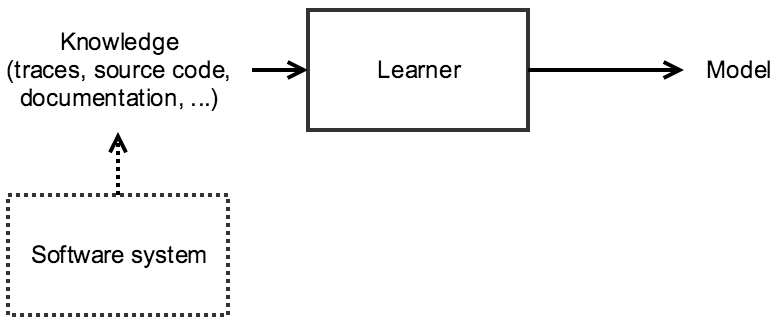
\includegraphics[width=0.9\linewidth]{figures/passive.png}
    \end{center}

    \caption{Passive model inference principle. The learner does
    not interact with the software system but rather relies on
    a fixed set of information (knowledge).}
    \label{fig:passive}
\end{figure}

The passive model inference category includes all techniques that
infer models from a fixed set of samples, such as a set of
execution traces, source code, or even documentation, as shown in
Figure \ref{fig:passive}. Since there is no interaction with the
system to model, theses techniques are said passive or offline.
In contrast to active model inference, the samples are usually
considered as positive elements. Also, models are often
constructed by initially representing sample sets with automata
whose equivalent states are merged. This section presents an
overview of these techniques.

A substantial part of the papers covering this topic proposes
approaches either based upon event sequence abstraction or
state-based abstraction to infer models. We introduce them in
Sections \ref{sec:passive-fsa} and \ref{sec:passive-spec}.
We present some white-box techniques, which retrieve
models from source code, in Section \ref{sec:passive-white}, as
well as a few alternative works leveraging documentation in
Section \ref{sec:passive-others}.

\subsubsection{Passive inference using event sequence abstraction}
\label{sec:passive-fsa}

Most of the following approaches, which build models from
execution traces by means of event sequence abstraction, are
build on-top of these two algorithms: \textit{kTail}
\cite{5009015} and \textit{kBehavior} \cite{mariani2007dynamic}.

kTail generates \textit{Finite State Automata} (FSA) from trace
sets in two steps. First, it builds a \textit{Prefix Tree
Acceptor} (PTA), which is a tree whose edges are labeled with
the event names found in traces. Then, kTail transforms the PTA
into a FSA by merging each pair of states as far as they exhibit
the same future of length $k$, i.e. if they have the same set of
event sequences having the maximum length $k$, which are all
accepted by the two states. This state merging step often yields
over-generalized models containing undesirable behaviors though
\cite{4023976}.

Reiss and Renieris modified the kTail algorithm to reduce the
size of the final FSA.  Indeed, their algorithm merges two states
if they share at least one \textit{k-future} \cite{919096}. By
using a merging criterion that is weaker, their variant actually
merges more states than kTail. Yet, the resulting FSA
express much more behaviors than those possible in the real
system. They are usually more approximate than the models
obtained with kTail. Lo et al. \cite{Lo:2009:ASB:1595696.1595761}
also enhanced the kTail algorithm to lower over-approximation.
Traces are mined to extract temporal properties that
statistically hold in most of the traces. Such temporal
properties aim at capturing relations between non consecutive
events. The kTail algorithm is then upgraded to prevent the
merging of states with the same k-future, which would produce FSA
that violate the inferred properties.

Lorenzoli et al. extended kTail to produce \textit{Extended
Finite State Machines} (EFSMs), which are FSMs extended with
parameters and algebraic constraints on transitions
\cite{Lorenzoli2008}. Their technique, called \textit{gkTail},
generates an EFSM from a set of traces, which incorporates
information about both the event sequences and the values of the
parameters associated with the event sequences. gkTail starts by
combining the traces that share the same event sequence, each
event being associated with the set of values obtained as the
union of all value assigned to this same event in each merged
trace. gkTail infers a constraint from the values associated with
each event, and combines this constraint with the associated
event. Finally, the kTail algorithm is applied on these traces.

\textit{kBehavior} \cite{mariani2007dynamic} is another
algorithm, which works quite differently than kTail. It generates
a FSA from a set of traces by taking every trace one after one,
and by completing the FSA such that it accepts the trace. More
precisely, whenever a new trace is submitted to kBehavior, it
first identifies the sub-traces that are accepted by sub-automata
in the current FSA (the sub-traces must have a minimal length
$k$, otherwise they are considered too short to be relevant).
Then, kBehavior extends the model with the addition of new
branches that connect the identified sub-automata,
producing a new version of the model that accepts the entire
trace. They successfully applied this algorithm to automatically
analyze log files and retrieved important information to identify
failure causes \cite{4700316}. They also automatically analyzed
logs obtained from workloads to highlight useful information that
can relate the failure to its cause
\cite{cotroneo2007investigation}. Both works
\cite{4700316,cotroneo2007investigation} use an extended version
of kBehavior, called \textit{kLFA}, that supports events
combined with data values. kLFA performs a preliminary step by
analyzing the traces to infer parameter constraints. It encodes
these constraints in the event names with specific symbols to
yield new traces. kBehavior is then called to infer a FSA whose
transitions are still labeled with an event and a symbol
representing a data constraint.

Lo et al. presented an empirical comparative study of kTail,
kBehavior, gkTail, and kLFA with a set of 10 case studies
extracted from real software systems in \cite{Lo20122063}. This
study quantifies both the effect of adding data flow information
within automata and the effectiveness of the techniques when
varying sparseness of traces. One of the main conclusions is that
adding algebraic constraints to FSA does not compromise quality
but negatively affects performance. This is the case for gkTail
for instance, which becomes extremely slow. The study also
revealed that increasing the trace set improves the rate of
correct behaviors in models, especially for kTail and kBehavior.
But increasing the trace set does not particularly affect illegal
behavior rates, i.e. the number of behaviors found in the models
but not in the traces. This can be explained by the fact that
these algorithms are not really able to control
over-generalization when only positive samples are available. A
comparison has also be made between the kTail- and
kBehavior-based methods. In short, kTail provides low illegal
behavior rate, but also low correct behavior rate. On the other
hand, kBehavior has higher illegal behavior rate, but good
correct behavior rate.

The next section gathers the approaches building models from
traces that also consider invariants to merge states.

\subsubsection{Passive inference using state-based abstraction}
\label{sec:passive-spec}

The approaches presented in this section rely on the generation
of state invariants to define equivalence classes of states that
are combined together to form final models. The \textit{Daikon}
tool \cite{Ernst:1999:DDL:302405.302467} was originally proposed
to infer invariants composed of data values and variables found
in execution traces. An invariant is a property that holds at a
certain point or points in a software. These are often used in
assert statements, documentation, and formal specifications. An
invariant generator mines the data found in the traces that a
software system produces, and then reports properties that are
$true$ over the observed executions.  This is a machine learning
technique that can be applied to arbitrary data. Daikon is used
in many different kinds of works, e.g., for generating test cases,
predicting incompatibilities in component integration, automating
theorem proving, repairing inconsistent data structures, and
checking the validity of data streams, among other tasks
\cite{Ernst200735}.

Krka et al. inferred object-level behavioral models (FSA) from
object executions, by using both invariants, representing object
states, and dynamic invocation sequences, expressing method
invocations \cite{Krka:2010:UDE:1810295.1810324}.
Invariants are still generated with Daikon. The authors show that
their FSA inference technique offers more precise models than
those obtained with kTail, which means that the rate of
over-approximation is lower. These results are not surprising
since they use a state merging technique combining event sequence
abstraction and state abstraction. Hence, state merging is here
done with more precision.

In \cite{Ghezzi:2009:SIB:1555001.1555057}, Ghezzi et al.
described an approach called \textit{SPY} to recover a
specification of a software component from its traces. They infer
a formal specification of stateful black-box components (Java
classes that behave as data containers with their own states).
Model inference is performed in two main steps. It starts by
building a DFA that models the partial behavior of the instances
of the classes. Then, the DFA is generalized via graph
transformation rules that are based upon the following
assumption: the behavior observed during the partial model
inference process benefits from the so called "continuity
property" (i.e. a class instance has a sort of "uniform"
behavior). Transformation rules generate data constraints that
hold for each encountered data value found in the instance pools.
Such constraints add over-approximation to the model though.

Walkinshaw et al. presented the \textit{Query-driven State
Merging} (QSM) algorithm in
\cite{Walkinshaw07reverseengineering}, an \textit{interactive}
grammar inference technique to infer the underlying state machine
representation of software. The QSM algorithm does not infer
invariants but uses the Price's "blue-fringe" state merging
algorithm \cite{Lang:1998:RAO:645517.655780}, which is mainly
based upon fixed invariants defining order relations over states.
QSM generalizes a supplied trace set obtained from an application
by applying two steps: (i) a trace abstraction is performed
with functions given by a user, and (ii) states are merged with
the Price's "blue-fringe" state merging algorithm. To avoid
over-generalization, the algorithm queries the user whenever the
resulting machine accept or reject sequences that have not
been ratified. This approach can be compared to the work done by
Hungar in \cite{hungar}, who used the $\EuScript{L}^*$ algorithm
instead. But the QSM algorithm presumes that the input sequences
offer some basic coverage of the essential functionality of the
system, in which case the machine can be inferred relatively
cheaply by a process of state merging, compared to the
$\EuScript{L}^*$ technique that systematically and
comprehensively explores the state space of the target machine.
Some tools such as \textit{Synapse}
\cite{LamelaSeijas:2014:SAB:2633448.2633457} implement the QSM
algorithm to perform automatic behavior inference and
implementation comparison for the programming language Erlang.

Taking another direction by leveraging genetic algorithms,
Tonella et al. \cite{TonellaNMLH13} applied a data-clustering
algorithm to infer FSMs from traces. Traces are transformed into a
first FSM where every state is considered as one distinct
equivalence class, called cluster. Then, invariants are generated
with Daikon for each cluster in order to group states. The
clustering is iteratively improved by using a genetic algorithm
that randomly update the clusters. But the clustering is yet
guided with the computation of quality attributes on the current
FSM model. Each distinct set of invariants produced for each
cluster at the end of the optimization represents an abstract
state, and is used as the abstraction function that maps states
to more abstract ones. Even though this approach offers
originality, it is time consuming, especially with a large set of
traces.

The works presented in this section adopted either a grey- or
black-box approach. The next section introduces some white-box
techniques.

\subsubsection{White-box techniques}
\label{sec:passive-white}

The works presented in this section adopt a white-box
perspective. Models are built by following two different
procedures: (i) the source code is instrumented and the system is
executed or tested to collect traces from which a specification
can be generated, and (ii) the source code is statically analyzed
to directly infer models.

Ammons et al. reuse the kTail algorithm to produce
non-deterministic automata from source code
\cite{Ammons:2002:MS:565816.503275}. The latter is instrumented
to collect the function calls and parameters.  Application traces
are collected and scenarios (small sets of interdependent
interactions) are then derived. kTail is finally employed to
build automata. Several automata are generated from the different
scenarios.

Whaley et al. suggested to use multiple FSM submodels to model
object-oriented component interfaces
\cite{Whaley:2002:AEO:566171.566212}. A FSM is built for each
attribute of a class, with one state per method that writes that
attribute. The FSMs are reduced with restrictions on the methods:
a distinction is made between side-effect-free methods, i.e. those
that do not change the object state, and the others. The
side-effect-free methods are ignored to build FSMs. The others are
completed with dotted transitions to represent the states
from which it is possible to call these side-effect-free methods.
Two techniques are given to automatically construct such models:
(i) a dynamic instrumentation technique that records real method call
sequences, and (ii) a static analysis that infers pairs of
methods that cannot be called consecutively. The work described
in \cite{Alur:2005:SIS:1047659.1040314} generates behavioral
interface specifications from Java classes by means of predicate
abstraction and active learning. This is a white-box approach
inspired by \cite{Whaley:2002:AEO:566171.566212} that, first,
uses \textit{predicate abstraction} to generate an abstract
version of the considered class. Afterwards, a minimal version
(interface) of this abstraction is constructed by leveraging the
$\EuScript{L}^*$ algorithm. The tool \textit{Java Interface
Synthesis Tool} (JIST) is the resulting implementation of such a
technique. It takes Java classes as input, and generates useful
and safe interfaces automatically.

Still in the purpose of modeling object invocation, Salah et al.
proposed \textit{Scenariographer} \cite{Salah05scenariographer},
an algorithm and a tool to estimate the usage scenarios of a
class from its execution profiles. The results are quite
different than the above approaches tough, since Scenariographer
infers a set of regular expressions expressing the generalized
usage scenarios of the class over its methods. The source code is
still instrumented to collect method calls, but this approach
employs the notion of canonical sets to categorize method
sequences into groups of similar sequences, where each group
represents a usage scenario for a given class.

Yang et al. \cite{Yang:2006:PMT:1134285.1134325} also focused on
the model inference of Java programs but they use a state
abstraction technique generating temporal invariants. The source
code is instrumented to collect method invocations. Then,
temporal invariants are extracted to capture relations among
several consecutive or non-consecutive events. The resulting tool
\textit{Perracotta} infers temporal invariants and FSMs from
traces. It is able to scale to large software systems since it
can infer models from millions of events. Additionally, it works
effectively with incomplete trace sets typically available in
industrial scenarios. Scalability is here obtained by the use of
heuristics to prune the set of inferred invariants.

In \cite{Pradel:2009}, Pradel and Gross presented a scalable
dynamic analysis that infers extremely detailed specifications of
correct method call sequences on multiple related objects. Again,
Java applications are executed to collect with debuggers methods
calls. This produces a large set of traces. Given that methods
generally implement small and coherent pieces of functionality,
the source code is statically analyzed to identify small sets of
related objects (object collaborations), and method calls that
can be analyzed separately. Then, they derive FSMs that model
legal sequences of method calls on a set of related objects. This
work has been extended in \cite{Dallmeier_generatingtest} by
means of active testing. The inference engine generates the test
cases that cover previously unobserved behaviors, systematically
extending the execution space and enriching the models while
detecting bugs. Such an approach is similar to the crawling
techniques presented in Section \ref{sec:active-crawling} except
that crawlers take GUI applications as input.

Even though the remaining papers are oriented towards the same
purpose, that is model inference from source code, they do not
collect traces from executions but perform static analysis only.
Shoham et al. introduced an approach to infer finite automata
describing method calls of an API from source code of the client
side, i.e. the code that calls the API
\cite{Shoham:2007:SSM:1273463.1273487}. Finite automata are
constructed with two main steps: (i) abstract-traces are
collected with a static analysis of the source code and split
into sets called abstract histories that give birth to several
finite automata, and (ii) a summarization phase filters out
noise. This step is done thanks to two available criteria: either
all the histories are considered (no filter) or the histories
having the same k-future (as with kTail) are assembled together.
Despite encouraging results, the inferred specifications are
often too detailed, and their solution does not scale well.

In \cite{Wasylkowski07detectingobject}, Wasylkowski et al.
proposed \textit{JADET}, a Java code analyzer to infer method
models. One finite state automaton is built for every class to
express the method calls. JADET then infers temporal properties
grouped into patterns that can be used to automatically find
locations in programs that deviate from normal object usage.
Temporal properties are obtained by the use of the data mining
technique frequent itemset mining, which is applied on the source
code. These properties are fed into a classifier that detects and
removes the abnormal properties. It then identifies the methods
that violate the remaining ones.

The next section introduces a few other works leveraging
documentation to infer models.

\subsubsection{Model inference from documentation}
\label{sec:passive-others}

We present in this section some other passive inference
techniques that rely on other sets of knowledge to infer models.
Their main disadvantage lies in the use of external documentation
that can be outdated, leading to models describing incorrect
behaviors (over-approximation). Furthermore, the resulting models
are often under-approximated since documentation is usually not
complete. That is probably why there are few works based on
documentation mining in the literature.

Bertolino et al. presented \textit{StrawBerry} in
\cite{Bertolino:2009:ASB:1595696.1595719}, a method that infers a
Behavior Protocol automaton from a Web Service Description
Language (WSDL) document.  WSDL is a format for documenting web
service interactions, containing information about the inputs,
outputs, and available methods. StrawBerry automatically derives a
partial ordering relation among the invocations of the different
WSDL operations, that is represented as an automaton called
Behavior Protocol automaton.  This automaton models the
interaction protocol that a client has to follow in order to
correctly interact with a web service.  The states of the
behavior protocol automaton are web service execution states, and
the transitions, labeled with operation names and input/output
data, model possible operation invocations from the client to the
web service.

Later, Zong et al. \cite{ZhongZXM11} proposed to infer
specifications from API documentation to check whether
implementations match it. A linguistic analysis is applied as API
documentation is written in a natural language. It results in a
set of methods that are linked together with action-resource
pairs that denote what action the method takes on which resource.
Then, a graph is built from these methods and a predefined
specification template. Such specifications do not reflect the
implementation behaviors though. Furthermore, this method can be
applied only if the API documentation is available in a readable
format, and if a specific template is provided.

In the sequel, we present two approaches combining model
inference and expert systems to infer models from traces for web
applications (Chapter \ref{sec:modelinf:webapps}) and industrial
systems (Chapter \ref{sec:modelinf:prodsystems}). The state
merging is replaced with a context-specific state reduction based
on an event sequence abstraction. This state reduction can be
seen as the kTail algorithm introduced previously where $k$ is as
high as possible. Furthermore, our work focus on both speed and
scalability to be able to construct models of Michelin's
production systems in an efficient manner. Among all potential
use cases, we need such models to perform passive testing on
these production systems.


% !TEX root = ../../thesis.tex
%
% !TEX root = ../../thesis.tex
%
\chapter{Model inference for web applications}
\label{sec:modelinf:webapps}

Over the last years, we developed an evolutive technique to infer
behavioral models of existing software systems. Our approach
relies on different techniques that we combined together in order
to build partial yet exact models of software systems.
Nonetheless, our target has always been to be able to construct
models of (legacy) production systems in an automated fashion.
But, before tackling the model inference of production systems,
we chose to validate our initial ideas and concepts by applying
them on web applications. That is the purpose of this chapter.

Web applications are often smaller and easier to understand than
production systems. The design of web applications is
well-established: we have a web server that runs the application,
no matter its underlying programming language, and a client (a
web browser most of the time) that connects to the web server so
that it can talk to the application. \textit{HyperText Transfer
Protocol} (HTTP) is the protocol that allows such a discussion by
means of HTTP requests and HTTP responses. Usually, the client
initiates a request, and the server responds to it. Requests
embed HTTP verbs (or methods), \textit{Unique Resource
Identifiers} (URIs also known as the "web links"), and sometimes
parameters along with their values. When one submits a
registration form on a web page, it is likely that the HTTP verb
is $POST$, and that there are at least as many parameters and
values as fields in the form. By clicking on the "submit" button
(or "save", "register", etc.), the web browser crafts an HTTP
request containing all the information, and sends it to the web
server that delivers the request to the application. When the
application sends back the appropriate response, it also goes
through the web server. By hooking between the web brower and the
web server, we are able to read both HTTP requests and responses
as far as there is no \textit{Secure Socket Layer} (SSL) or
\textit{Transport Layer Security} (TLS) involved, i.e. the
communication channel should not be encrypted.

We proposed a new approach to infer models of web applications,
which is divided into several modules as depicted in Figure
\ref{fig:soict-framework}. The \emph{Models generator} is the
centrepiece of this framework. It takes traces as inputs, which
can be sent by a \emph{Monitor} collecting them on the fly. Such
a monitor would be responsible for reading HTTP requests and
responses in our case. However, it is worth mentioning that the
traces can also be sent by any tool or even any user, as far as
they comply to a chosen standard format. The Models generator is
based upon an expert system, which is an artificial intelligence
engine emulating acts of a human expert by inferring a set of
rules representing his knowledge. Such knowledge is organised
into a hierarchy of several layers. Each layer gathers a set of
inference rules written with a first-order logic. Typically, each
layer creates a model, and the higher the layer is, the more
abstract the model becomes. Models are then stored and can be
later analysed by experts, verification tools, etc. The number of
layers is not strictly bounded even though it is manifest that it
has to be finite.

\begin{figure}[ht]
    \begin{center}
        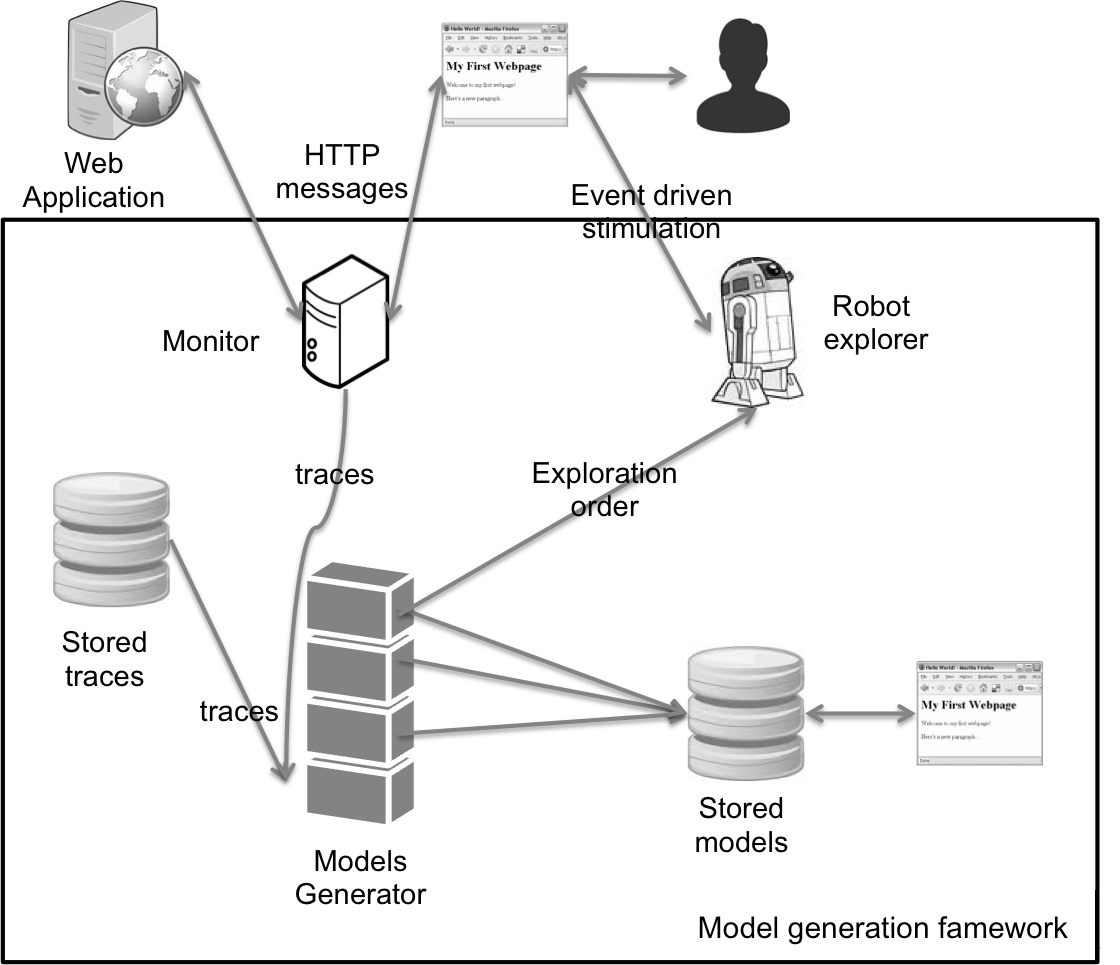
\includegraphics[width=0.8\linewidth]{figures/soict-framework.png}
    \end{center}
    \caption{Model generation framework for web applications}

    \label{fig:soict-framework}
\end{figure}

The Models generator relies upon traces to construct IOSTSs, but
the given trace set may not be substantial enough to generate
relevant IOSTSs. More traces could be yet collected as far as
the application being analysed is an event-driven application.
Such traces can be produced by stimulating and exploring the
application with automatic testing. In our approach, this
exploration is achieved by the \emph{Robot explorer}. In contrast
with most of the existing crawling techniques, which are detailed
in \crossref{sec:related}{sec:related:modelinf:crawling}, our
robot does not cover the application in blind mode or with a
static traversal strategy.  Instead, it is cleverly guided by the
Models generator, which applies an exploration strategy carried
out by inference rules.  This involves the capture of new traces
by the Monitor or by the Robot explorer which returns them to the
Models generator. The advantages of this approach are manifold:

\begin{itemize}
\item it takes a predefined set of traces collected from any kind
of applications producing traces. In the context of Web
applications, traces can be produced using automatic testing,

\item the application exploration is guided with a strategy which
can be modified according to the type of application being
analysed. This strategy offers the advantage of directly targeting
some states of the application when its state number is too large
for being traversed in a reasonable processing time,

\item the knowledge encapsulated in the expert system can be used
to cover trace sets of several applications belonging to the same
category with generic rules,

\item but, the rules can also be specialised and refined for one
application to yield more precise models. This is interesting for
application comprehension,

\item our approach is both flexible and scalable. It does not
produce one model but several ones, depending on the number of
layers of the Models generator, which is not limited and may
evolve in accordance to the application's type. Each model,
expressing the application's behaviours at a different level of
abstraction, can be used to ease the writing of complete formal
models, to apply verification techniques, to check the
satisfiability of properties, to automatically generate
functional test cases, etc.
\end{itemize}

We describe our work in the next section, then we present our
results in Section \ref{sec:modelinf:webapps:exp}, and we
conclude on this work in Section
\ref{sec:modelinf:webapps:conclusion}.

\textbf{Publication.} This work has been published in the
Proceedings of the Fifth Symposium on Information and
Communication Technology (SoICT'14)
\cite{DBLP:conf/soict/DurandS14}.

%%%%%%%%%%%%%%%%%%%%%%%%%%%%%%%%%%%%%%%%%%%%%%%%%%%%%%%%%%%%%%%%%

\section{Inferring models with rule-based expert systems}
\label{sec:modelinf:webapps:contrib}

\begin{figure}[ht]
    \begin{center}
        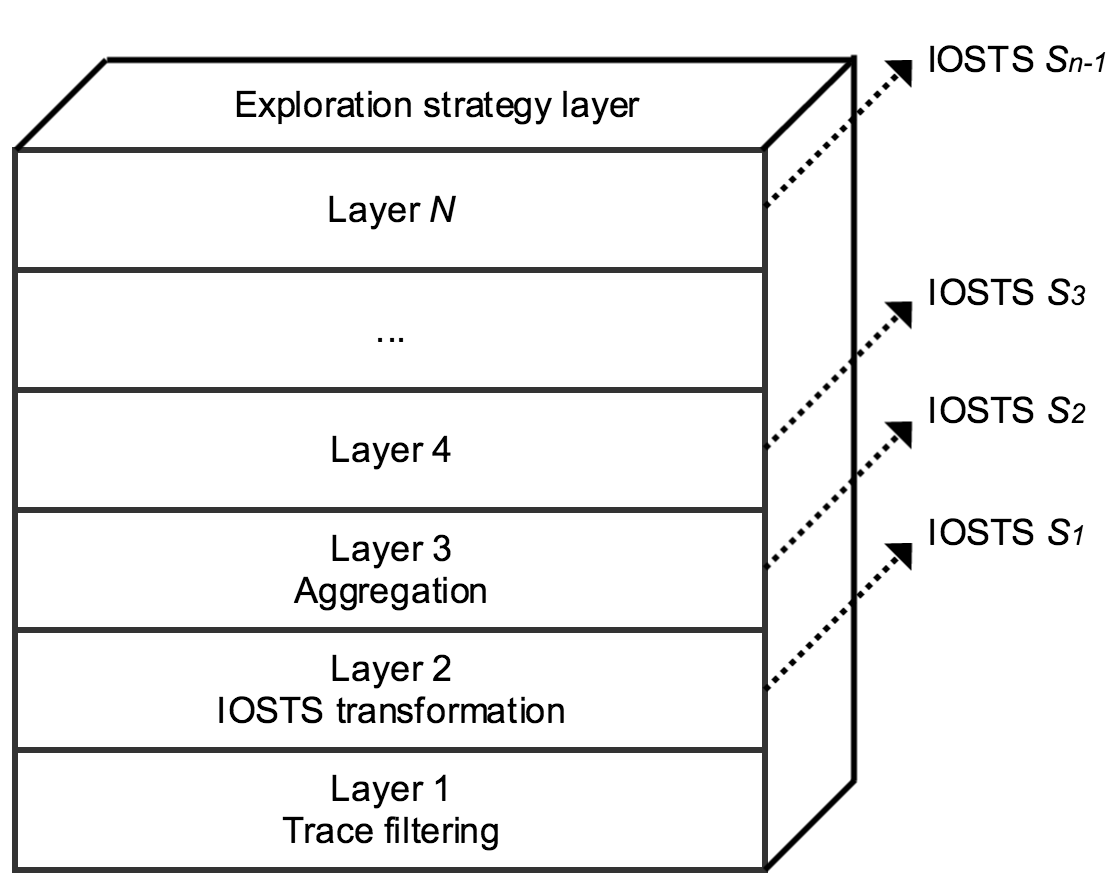
\includegraphics[width=1.0\linewidth]{figures/soict_se.png}
    \end{center}
    \caption {Models generator}

    \label{fig:se}
\end{figure}

The Models generator is mainly composed of a rule-based expert
system, adopting a forward chaining. Such a system separates the
knowledge base from the reasoning: the former is expressed with
data also known as facts and the latter is realised with
inference rules that are applied on the facts. Our Models
generator initially takes traces as an initial knowledge base and
owns inference rules organised into layers for trying to fit the
human expert behaviour. These layers are depicted in Figure
\ref{fig:se}.

Usually, when a human expert has to read traces of an
application, he often filters them out to only keep those which
make sense against the current application. This step is done by
the first layer whose role is to format the received raw traces
into sequences of valued actions and to delete those considered
as unnecessary. The implementation of this layer depends on the
nature of the input traces. The resulting structured trace set,
denoted $ST$, is then given to the next layer. This process is
incrementally done, i.e. every time new traces are given to the
Models generator, these are formatted and filtered before being
given to Layer 2. The remaining layers yield an IOSTS each
$\EuScript{S}_i (i\geq 1)$, which has a tree structure derived
from the traces. The role of Layer 2 is to carry out a first
IOSTS transformation from the structured traces. The next layers
3 to N (with N a finite integer) are composed of rules that
emulate the ability of a human expert to simplify transitions, to
analyse the transition syntax for deducing its meaning in
connection with the application, and to construct more abstract
actions that aggregate a set of initial ones. Theses deductions
are often not done in one step. This is why the Models generator
supports a finite but not defined number of layers.  Each of
these layers $i$ takes the IOSTS $\EuScript{S}_{i-1}$ given by
the direct lower layer. This IOSTS, which represents the current
base of facts, is analysed by the rules to infer another IOSTS
whose expressiveness is more abstract than the previous one. We
state that the lowest layers (at least Layer 3) should be
composed of generic rules that can be reused on several
applications of the same type. In contrast, the highest layers
should own the most precise rules that may be dedicated to one
specific application.

For readability purpose, we chose to represent inference rules
with this format: \emph{When conditions on facts Then actions on
facts}. This format has been borrowed to the Drools inference
engine \footnote{http://www.jboss.org/drools/}). Independently
on the application's type, Layers 2 to N handle the following
fact types: \emph{Location} which represents an IOSTS location,
and \emph{Transition}, which represents an IOSTS transition,
composed of two Locations Linit, Lfinal, and two data collections
Guard and Assign. Now, it is manifest that the inference of
models has to be done in a finite time and in a deterministic
way. To reach that purpose, we formulate the following hypotheses
on the inference rules:

\begin{enumerate}
\item (finite complexity): a rule can only be applied a limited
number of times on the same knowledge base,

\item (soundness): the inference rules are Modus Ponens (simple
implications that lead to sound facts if the original facts are
true: If P, then Q. P. Therefore, Q.),

\item (no implicit knowledge elimination): after the application
of a rule $r$ expressed by the relation $r: T_i \rightarrow
T_{i+1} (i\geq 2)$, with $T_i$ a Transition base, for all
transition $t=(l_n,l_m,a(p),G,A)$ extracted from $T_{i+1}$, $l_n$
is reachable from $l_0$.
\end{enumerate}

In the following, we illustrate each layer with examples.

\subsection{Layer 1: Trace filtering}
\label{sec:modelinf:webapps:L1}

Traces of Web applications are based upon the HTTP protocol,
conceived in such a way that each HTTP request is followed by
only one HTTP response. Consequently, the traces, given to Layer
1, are sequences of couples (HTTP request, HTTP response). This
layer begins formatting these couples so that these can be
analysed in a more convenient way.

An HTTP request is a textual message containing an HTTP verb
(also called method), followed by a Unique Resource Identifier
(URI). It may also contain header sections such as Host,
Connection, or Accept. The corresponding HTTP response is also a
textual message containing at least a status code. It may
encompass headers (e.g,.  Content-Type, Content-Length) and a
content. All these notions can be easily identified. For
instance, Figure \ref{fig:httpexample} depicts an HTTP request
followed by its response. This is a $GET$ HTTP request, meaning a
client wants to read the content of the $/hello$ resource, which
is, in this case, a web page in HTML.

\begin{figure}[ht]
\begin{framed}
\begin{BVerbatim}
GET /hello HTTP/1.1
Host: example.org
Connection: keep-alive
Accept: text/html
\end{BVerbatim}
\end{framed}

\begin{framed}
\begin{BVerbatim}
HTTP/1.1 200 OK
Content-Type: text/html
Content-Length: 13
Hello, World!
\end{BVerbatim}
\end{framed}

\caption{HTTP request/response example}
\label{fig:httpexample}
\end{figure}

For a couple \textit{(HTTP request, HTTP response)}, we extract
the following information: the HTTP verb, the target URI, the
request content which is a collection of data (headers, content)
and the response content which is the collection (HTTP status,
headers, response content). A header may also be a collection of
data or may be null. Contents are textual, e.g. HTML. Since
we wish to translate such traces into IOSTSs, we turn these
textual items into a structured valued action $(a(p),\theta)$
with $a$ the HTTP verb and $\theta$ a valuation over the variable
set $p=\{URI,request,response\}$. This is captured by the
following proposition:

\begin{definition}[Structured HTTP Traces] Let $t=
req_1,resp_1$, \dots, $req_n,$ $resp_n$ be a raw HTTP trace
composed of an alternate sequence of HTTP request $req_i$ and
HTTP response $resp_i$. The structured HTTP trace $\sigma$ of $t$
is the sequence $(a_1(p),\theta_1) \dots (a_n(p),\theta_n)$ where:

\begin{itemize}
\item $a_i$ is the HTTP verb used to make the request in $req_i$,

\item $p$ is the parameter set $\{URI, request, response\}$,

\item $\theta_i$ is a valuation $p \rightarrow D_p$ that assigns
a value to each variables of $p$.  $\theta$ is deduced from the
values extracted from $req_i$ and $resp_i$.
\end{itemize}

The resulting structured HTTP trace set derived from the raw HTTP
traces is denoted $ST$.
\end{definition}

If we take back the HTTP messages given in Figure
\ref{fig:httpexample}, we obtain the structured HTTP trace
$(Get(p), \theta)$ with $\theta = \{URI="/hello",
request=\{headers=[ Host= "example.org", Connection =
"keep-alive", Accept = "text/html" ]\},
response=\{statusCode=200, headers=[ Content-Type = "text/html",
Content-Length = 13], content= "Hello, World!"\}\}$.

For a main request performed by a user, many other sub-requests
are also launched by a browser in order to fetch images, CSS and
JavaScript files.  Generally speaking, these do not enlighten a
peculiar functional behaviour of the application. This is why we
propose to add rules in Layer 1 to filter these sub-requests out
from the traces. Such sub-requests can be identified by different
ways, e.g. by focusing on the file extension found at the end of
the URI or on the content-type value of the request headers.
Consequently, we created a set of rules, constituted of
conditions on the HTTP content found in an action, that remove
valued actions when the condition is met. A straightforward rule
example that removes the actions relative to the retrieval of PNG
images, is given in Figure \ref{fig:layer1:filter}.\\

\begin{figure}[ht]
\begin{framed}
\begin{BVerbatim}
rule "Filter PNG images"
when
  $va: Get(
    request.mime_type = 'png' or request.file_extension = 'png'
  )
then
  retract($va);
end
\end{BVerbatim}
\end{framed}

\caption{Filtering rule example that retracts the valued actions
related to PNG images}
\label{fig:layer1:filter}
\end{figure}

After the instantiation of the Layer 1 rules, we obtain a
formatted and filtered trace set $ST$ composed of valued actions.
At this point, we are ready to extract the first IOSTS.

\textit{Completeness, soundness, and complexity.} HTTP traces are
sequences of valued actions modelled with positive facts.
Typically, they form Horn clauses. Furthermore, inference rules
are Modus Ponens (soundness hypothesis). Consequently, Layer 1 is
sound and complete. Keeping in mind the finite complexity
hypothesis, its complexity is proportional to
$\EuScript{O}m(k+1)$ with $m$ the valued action number and $k$
the rule number. (at worst, every action is covered $k+1$ times).

\subsection{Layer 2: IOSTS transformation}
\label{sec:modelinf:webapps:L2}

The IOSTS transformation relies upon the IOLTS semantics
transformation that is achieved in a backward manner.  In order
to generate the first IOSTS denoted $\EuScript{S}_1$, the
associated runs are first computed from the structured traces by
injecting states between valued actions. These steps are detailed
in the following.

\subsubsection{Traces to runs}

Given a trace $\sigma$, a run $r$ is first derived by
constructing and injecting states on the right and left sides of
each valued action of $\sigma$. Keeping in mind the IOLTS
semantics definition, a state shall be modelled by the couple
$((URI,k),v_\emptyset)$ with $v_\emptyset$ the empty valuation.
$(URI,k)$ is a couple composed of a URI and of an integer $(k
\geq 0)$. Typically, a couple $(URI,k)$ shall be a location of
the future IOSTS. All the runs $r$ of $SR$ start with the same
state $(l0,v_\emptyset)$. Then, a run is constructed by
incrementally covering one trace: for an action $(a_i,\theta_i)$
found in a trace, we extract the valuation $URI=val$ from
$\theta_i$ giving the URI value of the next resource reached
after the action $a_i$, and we complete the current run $r$ with
$(a_i,\theta_i)$ followed by the state $((val,k),v_\emptyset)$.
Since we wish to preserve the sequential order of the actions
found in the traces, when a URI previously encountered is once
more detected, the resulting state is composed of the URI
accompanied with an integer $k$, which is incremented to yield a
new and unique state.

The translation of the structured traces into a run set is
performed by the Algorithm \ref{traces_to_runs}, which takes a
trace set $ST$ as input and returns a run set $SR$. It owns a
set $States$ storing the constructed states. All the runs $r$ of
$SR$ start with the same state $(l0,v_\emptyset)$. Algorithm
\ref{traces_to_runs} covers the actions $(a_i,\theta_i)$ of a
trace $\sigma$ in order to construct the next state $s$. It
extracts the valuation $URI=val$ (line 7) from $\theta_i$ giving
the URI value of the next resource reached after the action
$a_i$. The state $s=((val,k+1),v_\emptyset)$ is constructed with
$k$ such that there exists $((URI,k),v_\emptyset) \in States$
composed of the greatest integer $k \geq 0$. The current run $r$
is completed with the valued action $(a_i,\theta_i)$ followed by
the state $s$ (line 13). Finally, $SR$ gathers all the
constructed runs.

\begin{algorithm}
\SetKwInOut{Input}{input} \SetKwInOut{Output}{output}

\Input{Trace set $ST$}
\Output{Run set $SR$}

BEGIN\;

$States:=\emptyset$ is the set of the constructed states\;

\If{$ST$ is empty} {
$SR:= \{(l0,v_\emptyset)\}$}

\ForEach{trace $\sigma=(a_0,\theta_0)...(a_n,\theta_n) \in ST$} {
$r:= (l0,v_\emptyset)$\;

\For{ $0 \leq i \leq n$}{

extract the valuation $URI=val$ from $\theta_i$\;

\If{($(val,0),v_\emptyset) \notin States$}{
$s:=((val,0),v_\emptyset)$\; }

\Else{ $s:=((val,k+1),v_\emptyset)$ with $k\geq 0$ the greatest
integer such that $((val,k),v_\emptyset) \in States$\; }

$States:=States \cup \{s\}$\;

$r:=r.(a_i,\theta_i).s$

}%endfor_i

$SR:=SR \cup \{r\}$

}%endfor trace

END\;

    \caption{Traces to Runs Algorithm}
    \label{traces_to_runs}
\end{algorithm}

\begin{proposition}
For each trace $\sigma \in ST$, Algorithm \ref{traces_to_runs}
constructs a run $r=s_0(a_0,\theta_0)s_1 \dots
\\s_n(a_n,\theta_n)s_{n+1} \in SR$ such that $\forall
(a_i,\theta_i) ( 0<i\leq n), \exists ! s_i(a_i,\theta_i)s_{i+1}$
in $r$.
\end{proposition}

%%%%%%%%%%%%%%%%%%%%%%%%%%%%%%%%%%%%%%%%%%%%%%%%%%%%%%%%%%%%%%%%%

\subsubsection{IOSTS generation}
\label{sec:iosts-gen}

The first IOSTS $\EuScript{S}_1$ is derived from the run set $SR$
in which runs are disjoint except for the initial state
$(l0,v_\emptyset)$. Traces are translated into IOSTS paths that
are assembled together (IOSTS disjoint union). The IOSTS forms a
tree composed of paths, each expressing one trace, starting from
the same initial location.

\begin{definition}[IOSTS tree]
\label{IOSTS_tree}
Given a run set $SR$, the IOSTS $\EuScript{S}_1$ is called the
IOSTS tree of $SR$ and corresponds to the tuple
$<L_{\EuScript{S}_1}, l0_{\EuScript{S}_1},V_{\EuScript{S}_1},
V0_{\EuScript{S}_1}, I_{\EuScript{S}_1},
\Lambda_{\EuScript{S}_1},\rightarrow_{\EuScript{S}_1}>$ such
that:

\begin{itemize}

\item $L_{\EuScript{S}_1}= \{l_i \mid \exists r\in SR, (li,v_\emptyset)$ is
a state found in $r\}$,

\item $l0_{\EuScript{S}_1}$ is the initial location such that $\forall r \in
SR$, $r$ starts with $(l0_{\EuScript{S}_1},v_\emptyset)$,

\item $V_{\EuScript{S}_1}=\emptyset$, $V0_{\EuScript{S}_1}=v_\emptyset$,

\item $\Lambda_{\EuScript{S}_1}= \{a_i(p) \mid \exists r\in SR,
(a_i(p),\theta_i)$ is a valued action in $r\}$,

\item $\rightarrow_{\EuScript{S}_1}$ is defined by the following inference
rule applied on every element $r\in SR$:

\begin{tabular}{l}
$s_i (a_i(p),\theta_i) s_{i+1} \text{ is a term
of } r, s_i=(l_i,v_\emptyset),$
$s_{i+1}=(l_{i+1},v_\emptyset),$\\$ G_i=\displaystyle \bigwedge_{(x_i=vi)\in \theta_i} x_i==vi$
$\vdash$ $l_i \xrightarrow{a_i(p),G_i,(x:=x)_{x\in V}}_{\EuScript{S}_1} l_{i+1}$
\end{tabular}

\end{itemize}
\end{definition}

Here, locations could be merged to reduce the IOSTS size with the
classical learning algorithms based upon $\EuScript{L}^*$
\cite{Angluin198787,lambeau08}. Nonetheless, these would create
an extrapolation of this IOSTS. We prefer rejecting such a
solution to preserve the trace equivalence of the IOSTS
$\EuScript{S}_1$ against the structured trace set $ST$ before
applying inference rules. Instead, we propose to use a
minimisation technique.

\subsubsection{IOSTS minimisation}

This IOSTS tree can be reduced in term of location size by
applying a bisimulation minimisation technique which still
preserves the functional behaviours expressed in the original
model.  Intuitively, this minimisation constructs the state sets
(blocks) that are bisimilar equivalent. Two states are said
bisimilar equivalent, denoted $q \sim q'$ iff they simulate each
other and go to states from where they can simulate each other
again. Due to lack of room, we only refer to the bisimulation
minimisation algorithm of \cite{Fernandez89animplementation}.

When receiving new traces from the Monitor, the model yield by
this layer is not fully regenerated, but rather completed on the
fly. New traces are translated into IOSTS paths that are disjoint
from $\EuScript{S}_1$ except from the initial location. We
perform a union between $\EuScript{S}_1$ and IOSTS paths. Then,
the resulting IOSTS is minimised.

\textit{Completeness, soundness, complexity.} Layer 2 takes any
structured trace set obtained from HTTP traces. If the trace set
is empty then the resulting IOSTS $\EuScript{S}_1$ has a single
location $l_0$. A structured trace set is translated into an
IOSTS in finite time: every valued action of a trace is covered
once to construct states, then every run is lifted to the level
of one IOSTS path starting from the initial location. Afterwards,
the IOSTS is minimised with the algorithm presented in
\cite{Fernandez89animplementation}. Its complexity is
proportional to $\EuScript{O}(mlog (m+1))$ with $m$ the number of
valued actions. The soundness of Layer 2 is based upon the notion
of traces: an IOSTS $\EuScript{S}_1$ is composed of transition
sequences derived from runs in $SR$, itself obtained from the
structured trace set $ST$. As defined, the behaviours encoded in
$ST$ and $\EuScript{S}_1$ are equivalent since ordered runs are
transformed into ordered IOSTS sequences.

\begin{example}
We take as example a trace obtained from the GitHub website
\footnote{https://github.com/} after having executed the
following actions: login with an existing account, choose an
existing project, and logout. These few actions already produced
a large set of requests and responses. Indeed, a web browser
sends thirty HTTP requests on average in order to display a
GitHub page. The trace filtering from this example returns the
following structured traces where the request and response parts
are concealed for readability purpose:

\begin{figure}[ht]
\begin{BVerbatim}
Get(https://github.com/)
Get(https://github.com/login)
Post(https://github.com/session)
Get(https://github.com/)
Get(https://github.com/willdurand)
Get(https://github.com/willdurand/Geocoder)
Post(https://github.com/logout)
Get(https://github.com/)
\end{BVerbatim}
\end{figure}

After the application of Layer 2, we obtain the IOSTS given in Figure
\ref{fig:github:iosts:1}. Locations are labelled by the URI found
in the request and by an integer to keep the tree structure of
the initial traces. Actions are composed of the HTTP verb
enriched with the variables URI, request, and response. This
IOSTS exactly reflects the trace behaviour but is still difficult
to interpret. More abstract actions shall be deduced by the next
layers.
\end{example}

%%%%%%%%%%%%%%%%%%%%%%%%%%%%%%%%%%%%%%%%%%%%%%%%%%%%%%%%%%%%%%%%%

\subsection{Layers 3-N: IOSTS abstraction}
\label{sec:modelinf:webapps:L4}

As stated earlier, the rules of the upper layers analyse the
transitions of the current IOSTS for trying to enrich its
semantics while reducing its size. Given an IOSTS
$\EuScript{S}_1$, every next layer carries out the following
steps:

\begin{enumerate}
\item apply the rules of the layer and infer a new knowledge base
(new IOSTS $\EuScript{S}_i$, $i\geq 2$),

\item apply a bisimulation minimisation,

\item store the resulting IOSTS.
\end{enumerate}

Without loss of generality, we now restrict the rule structure to
keep a link between the generated IOSTSs. Thereby, every rule of
Layer $i$ ($i \geq 3$) either enriches the sense of the actions
(transition per transition) or aggregates transition sequences
into one unique new transition to make the resulting IOSTS more
abstract. It results in an IOSTS $\EuScript{S}_i$ exclusively
composed of some locations of the first IOSTS $\EuScript{S}_1$.
Consequently, for a transition or path of $\EuScript{S}_i$, we
can still retrieve the concrete path of $\EuScript{S}_1$. This is
captured by the following proposition:

\begin{proposition}
\label{prop:loc:inclu}
Let $\EuScript{S}_1$ be the first IOSTS generated from the
structured trace set $ST$. The IOSTS $\EuScript{S}_i (i>1)$
produced by Layer $i$ has a location set $L_{\EuScript{S}_i}$
such that $L_{\EuScript{S}_i} \subseteq L_{\EuScript{S}_1}$.
\end{proposition}

\textit{Completeness, soundness, complexity.} the knowledge base
is exclusively constituted by (positive) Transition facts that
have a Horn form. The rules of these layers are Modus Ponens
(soundness hypothesis). Therefore, these inference rules are
sound and complete. Furthermore, a behaviour encoded in an IOSTS
$\EuScript{S}_i$ cannot be lost in $\EuScript{S}_i$. With regards
to the (no implicit knowledge elimination) hypothesis and to
Proposition \ref{prop:loc:inclu}, the transitions of
$\EuScript{S}_i$ are either unchanged, enriched or combined
together into a new transition. The application of these layers
ends in a finite time (finite complexity hypothesis) and the
complexity of each is proportional to $\EuScript{O}m(k)$ with $m$
the transition number and $k$ the rule number.

\begin{figure}[H]
\begin{minipage}{.5\textwidth}
    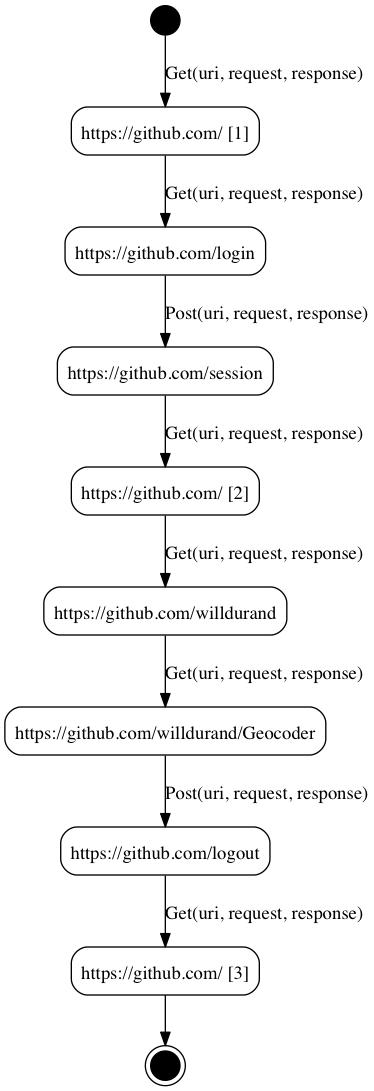
\includegraphics[width=0.8\linewidth]{figures/gh-iosts-1.png}

    \caption{IOSTS $\EuScript{S}_1$}
    \label{fig:github:iosts:1}
\end{minipage}
\begin{minipage}{.5\textwidth}
    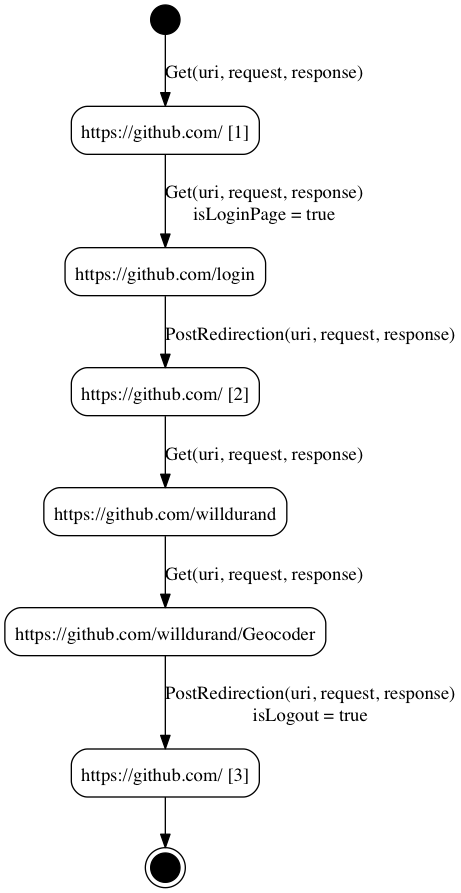
\includegraphics[width=1.0\linewidth]{figures/gh-iosts-2.png}

    \caption{IOSTS $\EuScript{S}_2$}
    \label{fig:github:iosts:2}
\end{minipage}
\end{figure}


\subsubsection{Layer 3}

It should correspond to a set of generic rules that can be
applied on a large set of applications belonging to the same
category. This layer has two roles:

\begin{itemize}
\item the \textbf{enrichment of the meaning captured in
transitions}. In this step, we chose to mark the transitions with
new internal variables. These shall help deduce more abstract
actions in the upper layers. These rules are of the form:

\begin{BVerbatim}
rule "Layer 3 rule"
when
  $t: Transition(conditions on action, Guard, Assign)
then
  modify ($t) {
    Assign.Add(new assignment over internal variables)
  };
end
\end{BVerbatim}

For example, the rules depicted in Figure \ref{fig:rule:login}
aims at recognising the receipt of a login or logout page. The
first rule means that if the response content, which is received
after a request sent with the $GET$ method, contains a login
form, then this transition is marked as a "login page" with the
assignment on the variable $isLoginPage$,

\item the \textbf{generic aggregation of some successive
transitions}. Here, some transitions (two or more) are analysed
in the conditional part of the rule. When the rule condition is
met then the successive transitions are replaced by one
transition carrying a new action. These rules have the following
form:

\begin{verbatim}
rule "Simple aggregation"
when
  $t1: Transition(
    conditions on action, Guard, ..., $lfinal := Lfinal
  )
  $t2: Transition(Linit == $lfinal, conditions)
then
  insert(new Transition(
    new Action,
    Guard($t1.Guard, t2.Guard),
    Assign($t1.Assign, $t2.Assignment),
    Linit == $t1.Linit,
    Lfinal == $t2.Lfinal
  ));
  retract($t1);
  retract($t2);
end
\end{verbatim}

The rule given in Figure \ref{fig:rule:redirect} corresponds to a
simple transition aggregation. It aims at recognising the
successive sending of information with a POST request followed by
a redirection to another Web page.  If a request sent with the
$POST$ method has a response identified as a redirection,
(identified by the status code 301 or 302), and  a $GET$ request
comes after, both transitions are reduced into a single one
carrying the new action $PostRedirection$.
\end{itemize}

\begin{figure}[h]
\begin{framed}
\begin{BVerbatim}
rule "Identify Login page"
when
  $t: Transition(
    Action == GET,
    Guard.response.content contains('login-form')
  )
then
  modify ($t) { Assign.add("isLoginPage := true") }
end
\end{BVerbatim}
\end{framed}

\begin{framed}
\begin{BVerbatim}
rule "Identify Logout action"
when
  $t: Transition(
    Action == GET,
    Guard.uri matches("/logout")
  )
then
  modify ($t1) { Assign.add("isLogout := true") }
end
\end{BVerbatim}
\end{framed}

\caption {Login page and logout action recognition rules}
\label{fig:rule:login}
\end{figure}

\begin{figure}[h]
\begin{framed}
\begin{BVerbatim}
rule "Identify Redirection after a POST"
when
  $t1: Transition(
    Action == POST,
    (Guard.response.status = 301 or Guard.response.status = 302),
    $l1final := Lfinal
  )
  $t2: Transition(
    Action == GET, linit == $l1final, $l2linit := Linit
  )
  not (Transition(Linit == $l2linit))
then
  insert(new Transition(
    "PostRedirection",
    Guard($t1.Guard, $t2.Guard),
    Assign($t1.Assign, $t2.Assign),
    $t1.Linit,
    $t2.Lfinal
  );
  retract($t1);
  retract($t2);
end
\end{BVerbatim}
\end{framed}

\caption{Simple aggregation to identify a redirection after a POST request}
\label{fig:rule:redirect}
\end{figure}

\begin{example}
When we apply these rules on the IOSTS example given in Figure
\ref{fig:github:iosts:1}, we obtain a new IOSTS illustrated in
Figure \ref{fig:github:iosts:2}. Its size is reduced since it has
6 transitions instead of 8 previously.  However, this new IOSTS
does not clearly reflect the initial scenario yet. Rules deducing
more abstract actions are required. These are found in the next
layer.
\end{example}

\subsubsection{Layer 4}

This layer aims at inferring a more abstract model composed of
more expressive actions and whose size should be reduced. Its
rules may have different forms:

\begin{itemize}
\item they can be applied on a single transition only. In this
case, the rule replaces the transition action to add more sense
to the action. The rule given in Figure \ref{fig:rule:deauth} is
an example which recognises a user de-authentication and adds a
new action "Deauthentication". This rule means that if a
$PostRedirection$ action is triggered against a "Logout" endpoint
(given by the variable \emph{isLogout} added by Layer 3), then
this is a deauthentication,

\item the rules can also aggregate several successive transitions
up to complete paths into one transition labelled by a more
abstract action. For instance, the rule illustrated in Figure
\ref{fig:rule:auth} recognises a user authentication thanks to
the variable $isLoginPage$ added by Layer 3. This rule means that
if a "Login" page is displayed, followed by a redirection
triggered by a $POST$ request, then this is an authentication
step, and the two transitions are reduced into a single one
composed of the action "Authentication".
\end{itemize}

\begin{figure}[h]
\begin{framed}
\begin{BVerbatim}
rule "Identify Deauthentication"
when
  $t: Transition(
    action == PostRedirection,
    Assign contains "isLogout:=true"
  )
then
  modify ($t) { $t.setAction("Deauthentication") };
end
\end{BVerbatim}
\end{framed}

\caption{Deauthentication recognition rule}
\label{fig:rule:deauth}
\end{figure}

\begin{figure}
\begin{framed}
\begin{BVerbatim}
rule "Identify Authentication"
when
  $t1: Transition(
    Action == GET,
    Assign contains "isLoginPage:= true",
    $t1final := Lfinal
  )
  $t2: Transition(
    Action == PostRedirection,
    Linit == $t1lfinal,
    $t2linit := Linit
  )
  not (Transition (Linit == $t2linit))
then
  insert(new Transition(
    "Authentication",
    Guard($t1.Guard,$t2.Guard),
    Assign($t1.Assign, $t2.Assign),
    $t1.Linit,
    $t2.Lfinal
  );
  retract($t1);
  retract($t2);
end
\end{BVerbatim}
\end{framed}

\caption{Authentication recognition}
\label{fig:rule:auth}
\end{figure}

Other rules can also be application-specific, so that these bring
specific new knowledge to the model. For instance, the GitHub Web
application has a dedicated URL grammar (a.k.a. routing system).
GitHub users own a profile page that is available at:
\emph{https://github.com/\{username\}} where \emph{\{username\}}
is the nickname of the user. However, some items are reserved,
e.g. \textit{edu} and \textit{explore}. The rule given in Figure
\ref{fig:rule:gh-profile} is based upon this structure and
produces a new action $ShowProfile$ offering more sense.
Similarly, a GitHub page describing a project has a URL that
always matches the pattern:
\emph{https://github.com/\{username\}/\{project\_name\}}. The
rule given in Figure \ref{fig:rule:gh-project} captures this
pattern and derives a new action named $ShowProject$.

\begin{figure}
\begin{framed}
\begin{BVerbatim}
rule "GitHub profile pages"
when
  $t: Transition(
    action == GET,
    (Guard.uri matches "/[a-zA-Z0-9]+$",
     Guard.uri not in [ "/edu", "/explore" ])
  )
then
  modify ($t) { $t.setAction("ShowProfile") };
end
\end{BVerbatim}
\end{framed}

\caption{User profile recognition}
\label{fig:rule:gh-profile}
\end{figure}

\begin{figure}
\begin{framed}
\begin{BVerbatim}
rule "GitHub project pages"
when
  $t: Transition(
    action == GET,
    Guard.uri matches "/[a-zA-Z0-9]+/.+$",
    $uri := Guard.uri
  )
then
  String s = ParseProjectName($uri);
  modify ($t) {
    $t.setAction("ShowProject");
    Assign.add("ProjectName := " + s);
  }
end
\end{BVerbatim}
\end{framed}

\caption{Project choice recognition}
\label{fig:rule:gh-project}
\end{figure}

\begin{example}
The application of the four previous rules leads to the final
IOSTS depicted in Figure \ref{fig:github:iosts:4}. Now, it can be
used for application comprehension since most of its actions have
a precise meaning and clearly describe the application's
behaviours.
\end{example}

\begin{figure}[ht]
    \begin{center}
    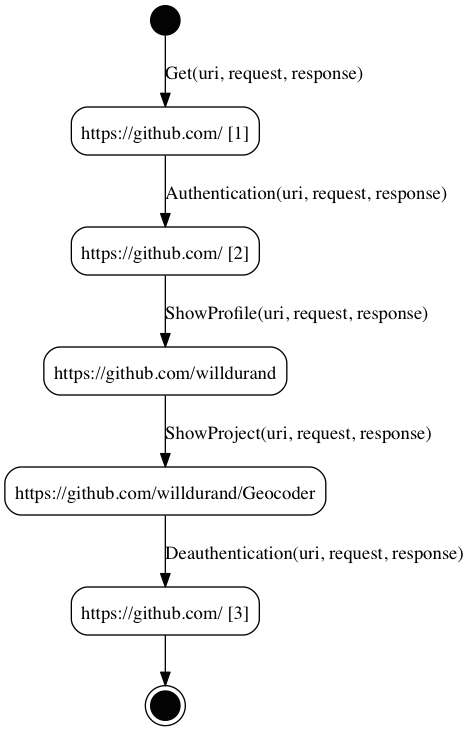
\includegraphics[width=0.6\linewidth]{figures/gh-iosts-41.png}
    \caption {IOSTS $\EuScript{S}_3$}
    \label{fig:github:iosts:4}
    \end{center}
\end{figure}

\subsection{Strategy layer}
\label{sec:modelinf:webapps:strategy}

Rather than using a static traversal strategy as in
\cite{Memon:2003,concolicandroid12,crawljax:tweb12,
Amalfitano:2012:UGR:2351676.2351717, WPX13}, we propose the
addition of an orthogonal layer in the Models generator to
describe any kind of exploration strategy by means of rules.

The simplified Algorithm of the Strategy layer is given in
Algorithm \ref{Exploration Strategy}. The latter applies the
rules on any stored IOSTS $\EuScript{S}_i$. It emerges a
location list $Loc$ that are marked with "explored" by the rules
to avoid re-using them twice (line 4). Then, the algorithm goes
back to the first generated IOSTS $\EuScript{S}_1$ in order to
extract one complete and executable path $p$ ended by a location
$l$ of $Loc$ (line 7). This step is sound since all the locations
of $\EuScript{S}_i$ belong to the location set of
$\EuScript{S}_1$ (Proposition \ref{prop:loc:inclu}). Such an
IOSTS preamble is required by the Robot explorer for trying to
reach the location $l$ by executing every action of $p$. The
algorithm finally returns a list of paths $List$, which is sent
to the Robot explorer. The exploration ends once all the
locations of $\EuScript{S}_i$ or of $\EuScript{S}_1$ are visited
(line 3). The algorithm only returns unexplored locations even
if, while the execution of the algorithm, the IOSTS
$\EuScript{S}_i$ has been regenerated several times since the
marked locations are also stored in the set $L$. Hence, if a
location of $\EuScript{S}_i$ is chosen a second time by the
rules, the algorithm checks if it has been previously visited
(line 7).

\begin{algorithm}
\SetKwInOut{Input}{input} \SetKwInOut{Output}{output}

\Input{IOSTS $\EuScript{S}_1$, $\EuScript{S}_i$}
\Output{List of preambles}

$L:=\emptyset$ List of explored locations of $\EuScript{S}_1$\;
BEGIN\;
\While{$L \neq L_{\EuScript{S}_1}$ and $L \neq \EuScript{S}_i$ }
{
1) Apply the rules on $\EuScript{S}_i$ and extract a  Location List $Loc$\;
Goback to $\EuScript{S}_1$\;

\ForEach{$l \in Loc$}{
\If{$l \notin L$}
{Compute a preamble $p$ from $l0_{\EuScript{S}_1}$ which reaches $l$\;

$L:= L \cup \{l\}$\;
$List:= List \cup  \{p\}$\;
}
%\Else{Repeat 1)}
}
}
END\;

\caption{Exploration Strategy}
 \label{Exploration Strategy}
\end{algorithm}

The rules of the Strategy layer can encode different strategies.
We propose two examples below:
\begin{itemize}

\item \textbf{classical traversal strategies} can still be
established.  For example, Figure \ref{fig:rule:bfs} depicts two
rules expressing the choice the next location to explore in a
breadth-wise order first. First, the initial location $l0$ is
chosen and marked as explored (rule BFS).  Then, the transitions
having an initial location marked as explored and a final
location not yet explored are collected by the rule BFS2, except
for the transitions carrying an HTTP error (response status upper
or equal to 400).  These locations are marked as explored in the
IOSTS $\EuScript{S}_i$ with the method $SetExplored$ in the
"then" part of the rule,

\item \textbf{semantic-driven strategies} could also be applied,
when the meaning of some actions is recognisable. For instance,
for e-commerce applications, the login step and the term "buy"
are usually important. Thereby, a strategy targeting firstly the
locations of transitions carrying theses actions can be defined
by the rule "semantic-driven strategy" given in Figure
\ref{fig:rule:semdriven}.
It is manifest that the semantic-driven strategy domain can be
tremendously vast since it depends on the number of recognised
actions and on their relevance.
\end{itemize}

\begin{figure}[h]
\begin{framed}
\begin{BVerbatim}
rule "BFS"
when
  $l: Location(name == l0, explored == false)
then
  $l.SetExplored();
end
\end{BVerbatim}
\end{framed}

\begin{framed}
\begin{BVerbatim}
rule "BFS2"
when
  $Loc: ArrayList<Location>() from accumulate(
    $t: Transition(Guard.response.status > 199
      && Guard.response.status < 400
      && Linit.explored == true
      && Lfinal.explore==false
    ),
    init(ArrayList<Transition> Loc = new ArrayList<Transition>()),
    action(Loc.add($t.Lfinal)),
    result(Loc)
  )
then
  Loc.SetExplored();
end
\end{BVerbatim}
\end{framed}

\caption{BFS strategy}
\label{fig:rule:bfs}
\end{figure}

\begin{figure}[h]
\begin{framed}
\begin{BVerbatim}
rule "semantic-driven strategy"
when
  $t: Transition (
    Assign contains "isLogin := true"
    or Guard.response matches "*buy*"
  )
then
  ArrayList Loc = new ArrayList();
  Loc.add($t.Linit, $t.Lfinal);
  Loc.SetExplored();
end
\end{BVerbatim}
\end{framed}

\caption{Semantic-driven strategy}
\label{fig:rule:semdriven}
\end{figure}

Many other strategies could be defined in relation to the desired
result in terms of model generation and application coverage.
Other criteria, e.g. the number of UI elements per Graphical User
Interface (GUI) or the number of observed crashes could also be
taken into consideration.

%%%%%%%%%%%%%%%%%%%%%%%%%%%%%%%%%%%%%%%%%%%%%%%%%%%%%%%%%%%%%%%%%

\section{Implementation and experimentation}
\label{sec:modelinf:webapps:exp}

We implemented this technique in a prototype tool called
\emph{Autofunk}. A user interacts with Autofunk through a Web
interface and either gives a URL  or a file containing traces.
These have to be stored in the HTTP Archive (HAR) format as it is
the defacto standard to describe HTTP traces, used by various
HTTP related tools. Such traces can be obtained from many HTTP
monitoring tools (Mozilla Firefox or Google Chrome included).
Then, Autofunk produces IOSTS models which are stored in a
database. The last model is depicted in the Web interface. The
JBoss Drools Expert tool has been chosen to implement the
rule-based system. Such an engine leverages Object Oriented
Programming in the rule statements and takes knowledge bases
given as Java objects (Location, Transition, GET, POST objects in
this work).

The GitHub website \footnote{https://github.com/} is an example
of application giving significant results. We recorded a trace
set composed of 840 HTTP requests / responses. Then, we applied
Autofunk on them with a Models generator composed of 5 layers
gathering 18 rules whose 3 are specialised to GitHub. After
having performed trace filtering (Layer 1), we obtained a first
IOSTS tree composed of 28 transitions. The next 4 layers
automatically inferred a last IOSTS tree $\EuScript{S}_4$, given
in Figure \ref{fig:git:iosts}, that is composed of 12 transitions
from which 9 have a clear and intelligible meaning.

\begin{figure}[ht]
    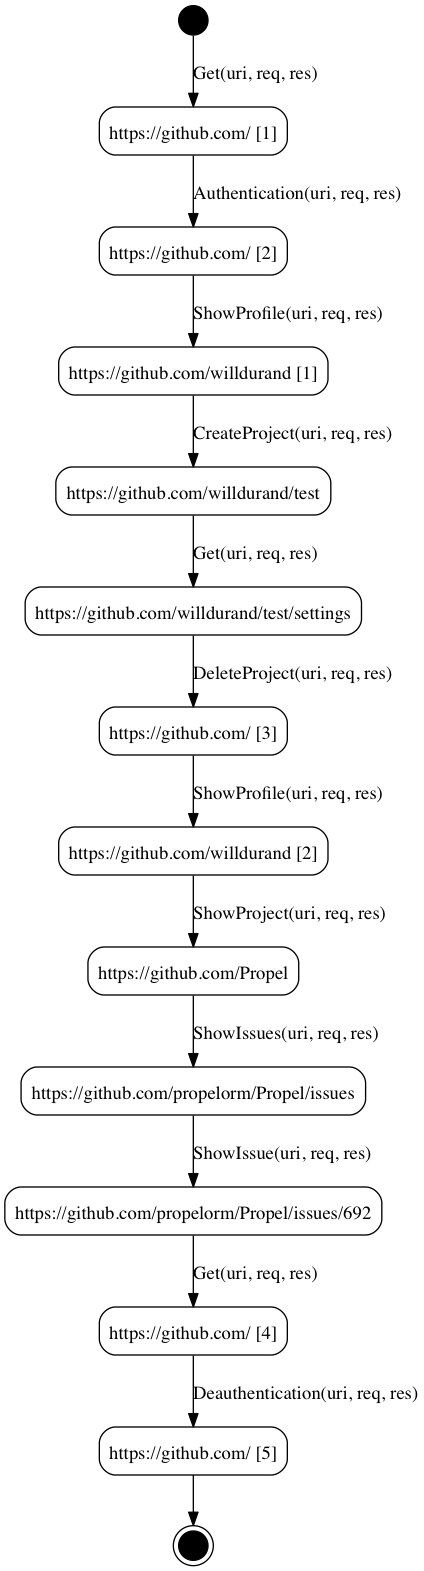
\includegraphics[width=.45\textwidth]{figures/gh-2-4-bis.png}

    \caption {Final IOSTS $\EuScript{S}_4$}
    \label{fig:git:iosts}
\end{figure}

%%%%%%%%%%%%%%%%%%%%%%%%%%%%%%%%%%%%%%%%%%%%%%%%%%%%%%%%%%%%%%%%%

\section{Conclusion}
\label{sec:modelinf:webapps:conclusion}

In this chapter, we presented an original approach combining
model inference, expert systems and automatic testing to derive
IOSTSs models. Our proposal yields several models, reflecting
different levels of abstractions of the same application with the
use of inference rules that capture the knowledge of an expert.
The first contribution lies in the flexibility and scalability
brought by the inference rules since they can be applied on
several applications or on a single application only when the
rules are specific. The whole framework has not to be
re-implemented for each application. Our approach can be applied
on event-driven applications since our framework supports their
exploration. Furthermore, it can also be applied on other kinds
of application as far as they produce traces.

While the idea of getting more and more abstract models was
interesting to us, we chose to stop working on this part as our
industrial partner was less interested in the part than on the
others. On the contrary, the first results on model inference
were very encouraging, so we decided to rework our architecture
to build a better framework on top of this one in order to
construct models of production systems. That is the purpose of
the next chapter.

\chapter{Model inference for production systems}
\label{sec:modelinf:prodsystems}

In this chapter, we introduce \emph{Autofunk v2}, following by
\emph{Autofunk v3}. This is our passive model inference
framework, improving \emph{Autofunk v1}'s capabilities, and
focused on inferring models of production systems. It combines
model inference, machine learning, and expert systems to infer
Symbolic Transition Systems (STSs). We replaced the minimization
technique presented in the previous chapter by a context-specific
reduction method, still preserving exactness of the inferred
models, but more efficient. This is illustrated with an
evaluation of \emph{Autofunk v2}. These results conducted to
the release of \emph{Autofunk v3}.  The main difference between
\emph{Autofunk v2} and \emph{Autofunk v3} is the use of the
\emph{k-means clustering} method. This is a machine learning
technique that we leverage to segment and filter input trace
sets, so that inferred models contain complete behaviors only.\\

\minitoc

\pagebreak

\section{Introduction}

In the Industry, building models for production systems,
\emph{i.e.} event-driven systems that run in production
environments and are distributed over several devices and
sensors, is frequent since these are valuable in many situations
like testing and fault diagnosis for instance. Models may have
been written as storyboards or with languages such as the \emph{Unified
Modeling Language} (UML) or even more formal languages. Usually,
these models are designed when brand-new systems are built. It
has been pointed out by our industrial partner that production
systems have a life span of many years, up to 20 years, and are
often incrementally updated, but their corresponding models are
not.  This leads to a major issue which is to keep these models
up to date and synchronized with the respective systems. This is
a common problem with documentation in general, and it often
implies rather under-specified or not documented systems that no
one wants to maintain because of lack of understanding.

In this chapter, we focus on this problem for production systems
that exchange thousands of events a day. Several approaches have
already been proposed for different types of systems.  Yet, we
noticed that these approaches were not tailored to support
production systems. From the literature,
\crossref{sec:related}{sec:related:modelinf}, we deduced the
following key observations:

\begin{itemize}
    \item Most of the existing model inference approaches give
        approximate models capturing the behaviors of a system
        and more. In our context, we want exact models that could
        be used for regression test case generation, and fault
        diagnosis. We define exactness with the
        \emph{trace-inclusion} and \emph{trace-equivalence}
        relations given in \cite{petrenko06};

    \item Applying active inference on running systems is
        complicated since these must not be disrupted (otherwise
        it may lead to severe damages on the production
        machines), but also because we cannot rely on any oracle
        or teacher;

    \item Production systems exchange thousands and thousands of
        events a day. Again, most of the model inference
        approaches cannot take such a huge amount of information
        to build models. We need a solution that is scalable.
\end{itemize}

Based on these observations, we propose a pragmatic \emph{passive
model inference} approach that aims at building formal models
describing functional behaviors of a system. Our goal is to
quickly build exact models from large amounts of production
events.  Furthermore, execution speed takes an important place
for building up to date models. Such models could also be used
for diagnosis every time an issue would be experienced in
production.  The strong originality of our approach lies in the
combination of two domains for model inference: model-driven
engineering and expert systems. We consider formal models and
their definitions to infer models by means of different
transformations. But we also take into consideration the
knowledge of human experts captured by expert systems. A part of
our approach is based upon this notion of knowledge implemented
with inference rules. We reuse what worked well for web
applications and enhance many parts of our framework to come up
with a better version of our \textit{Autofunk} framework, which
is presented throughout this thesis.

In the following section, we describe the context in which this
work has been conducted. In Section
\ref{sec:modelinf:prodsystems:autofunk}, we present
\textit{Autofunk} for Michelin's production systems along with a
case study. Section \ref{sec:modelinf:usability} highlights our
work on improving usability of the generated models.  We give our
results in Section \ref{sec:modelinf:prodsystems:results}. We
highlight an improvement made on our framework in Section
\ref{sec:modelinf:prodsystems:better-segmentation}, which is
part of \emph{Autofunk v3}. We conclude on this chapter in
Section \ref{sec:modelinf:prodsystems:conclusion}.

\textbf{Publications.} This work has been published in the
Proceedings of Formal Methods 2015 (FM'15)
\cite{DBLP:conf/fm/DurandS15}, and in the Proceedings of the 9th
International Conference on Distributed Event-Based Systems
(DEBS'15) \cite{DBLP:conf/debs/SalvaD15}.

\section{Context at Michelin}
\label{prodsys:context}

Michelin is a worldwide tire manufacturer and designs most of its
factories, production systems, and software by itself.  Like
many other industrial companies, Michelin follows the \emph{Computer
Integrated Manufacturing} (CIM) approach \cite{rehg2004computer},
using computers and software to control the entire manufacturing
process. In this thesis, we focus on the Level 2 of the CIM
approach, \emph{i.e.} all the applications that monitor and control
several production devices and \emph{points}, \emph{i.e.}
locations where a production line branches into multiple lines,
in a workshop. In a factory, there are different \emph{workshops}
for each step of the tire building process. At a workshop level,
we observe a continuous stream of products from specific entry
points to a finite set of exit points, \emph{i.e.} where products
go to reach the next step of the manufacturing process, and
disappear of the workshop frame in the meantime, as shown in
Figure \ref{fig:workshop-annotated}.  Depending on the workshops,
products can stay in this frame for days up to several weeks.
Indeed, a workshop may contain storage areas where products can
stay for a while, depending on the production campaigns or needs
for instance.  Thousands and thousands of \emph{production
events} are exchanged among the industrial devices of the same
workshop every day, allowing some factories to build over 30,000
tires a day.

\begin{figure}[ht]
    \begin{center}
        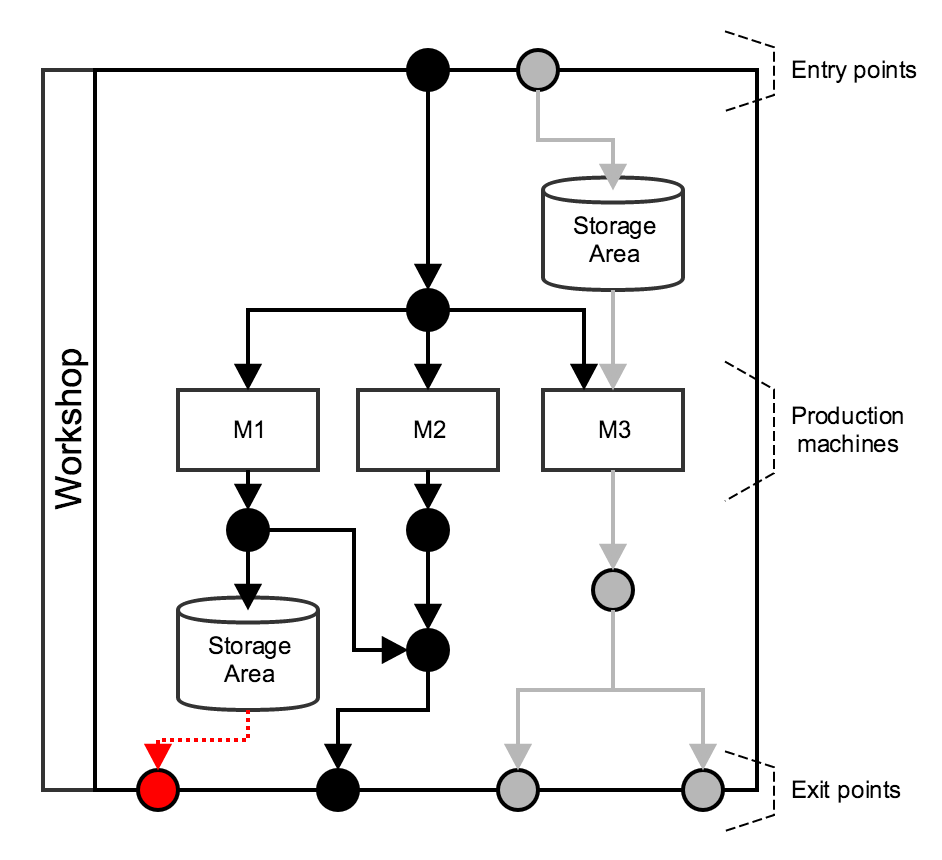
\includegraphics[width=1.0\linewidth]{figures/workshop-annotated.png}
    \end{center}

    \caption{A workshop owns a set of known entry and exit
    points. A continuous stream of products starts from known
    entry points, and ends at known exit points. This figure
    shows two production lines: the grey line having two exit
    points (represented by the circles), and the black one having
    only one real exit point, not two. The red dotted line
    represents a false-positive here, which is a problem we have
    to take into account while detecting (entry and) exit
    points.}
    \label{fig:workshop-annotated}
\end{figure}

Although there is a finite number of applications, each has
different versions deployed in factories all over the world,
potentially highlighting even more different behaviors and
features. Even if a lot of efforts are put into standardizing
applications and development processes, different programming
languages and different frameworks are used by development
teams, making difficult to focus on a single technology. Last
but not least, the average lifetime of these applications is 20
years. This set is large and too disparate to apply conventional
testing techniques, yet most of the applications exchange events
using dedicated custom internal protocols.

Our industrial partner needs a safe way to infer up to date
models, independent of the underlying technical details, and
without having to rely on any existing documentation.
Additionally, Michelin is interested in building regression test
suites to decrease the time required to deploy or upgrade
systems. We came up to the conclusion that, in order to target
the largest part of all Michelin's Level 2 applications, taking
advantage of the production events exchanged among all devices
would be the best solution, as it would not be tied to any
programming language or framework, and these events contain all
information needed to understand how a whole industrial system
behaves in production. All these events are collected
synchronously through a (centralized) logging system. Such a
system logs all events with respect to their order, and does not
miss any event.  From these, we chose not to use extrapolation
techniques to infer models, meaning our proposal generates
exact models, exclusively describing what really happens
in production.

This context leads to some assumptions that have been considered
to design our framework:

\begin{itemize}
    \item \textbf{Black-box systems:} production systems are seen as
        black-boxes from which a large set of production events can
        be passively collected. Such systems are compound of
        production lines fragmented into several devices and sensors.
        Hence, a production system can have several entry and exit
        points. We denote such a system by $\mathit{Sua}$ (\emph{system
        under analysis});

    \item \textbf{Production events:} an event of the form
        $a(\alpha)$ must include a distinctive label $a$ along with a
        parameter assignment $\alpha$. Two events $a(\alpha_1)$ and
        $a(\alpha_2)$ having the same label $a$ must own assignments
        over the same parameter set. The events are ordered and
        processed with respect to this order;

    \item \textbf{Traces identification:} traces are sequences of
        events $a_1(\alpha_1) \dots  a_n(\alpha_n)$. A
        trace is identified by a specific parameter that is
        included in all event assignments of the same trace. This
        identifier is denoted by $pid$ and identifies products,
        \emph{e.g.}, tires at Michelin.  Besides this, event
        assignments include a time stamp to sort the events into
        the traces.
\end{itemize}

%%%%%%%%%%%%%%%%%%%%%%%%%%%%%%%%%%%%%%%%%%%%%%%%%%%%%%%%%%%%%%%%%

\section{\textit{Autofunk}'s models generator revisited}
\label{sec:modelinf:prodsystems:autofunk}

In this section, we introduce our framework \textit{Autofunk v2},
whose main architecture is depicted in Figure
\ref{fig:prodsystems:autofunk-overview}. This new version also
contains different modules (in grey in the figure): four modules
are dedicated to build models, and an optional one can be used to
derive more abstract and readable models.

\begin{figure}[ht]
    \begin{center}
        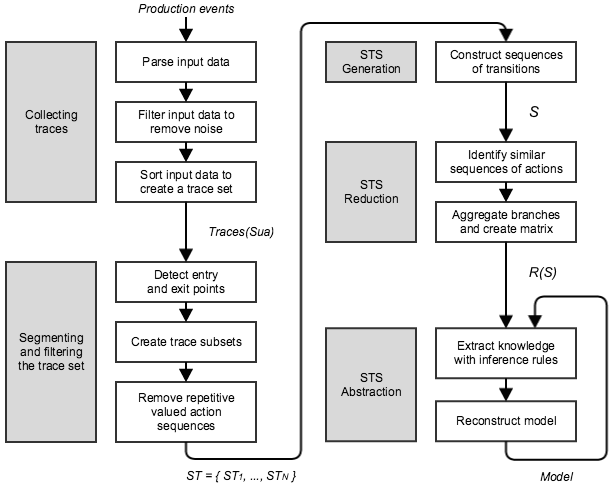
\includegraphics[width=1.0\linewidth]{figures/autofunk.png}
    \end{center}

    \caption{Overview of \textit{Autofunk v2}. It is a set of
    different modules (in grey) along with their corresponding
    steps. The last module (STS abstraction) is optional.}
    \label{fig:prodsystems:autofunk-overview}
\end{figure}

Here, we consider \textit{Symbolic Transition Systems} (STSs) as
models for representing production system behaviors. As reminder,
STSs are state machines incorporating actions (\emph{i.e.} events
in this context), labeled on transitions, that show what can be
given to and observed on the system. In addition, actions are
tied to an explicit notion of data. A formal definition can
be found in \crossref{sec:related}{sec:definitions:sts}.
The innovation of this framework lies in the combination of the
notion of expert systems with the STS formalism: the STS
representation, operators and transformations, are expressed
with deduction rules, and the knowledge of a human expert of a
system can be transcribed with inference rules.
\textit{Autofunk v2} combines both domains in such a way that
each model modification can be expressed and implemented with a
rule.  As a consequence, the data collections handled by
\textit{Autofunk} are always expressed with knowledge bases
(Events, Actions, Traces, STSs, etc.) on which rules are applied
to infer models. Given a system $\mathit{Sua}$ and a set of
production events, \textit{Autofunk} builds \emph{trace-included}
models, \emph{i.e.} the traces of a model $\EuScript{S}$ are
included in the traces of $\mathit{Sua}$.

\begin{figure}[ht]
\begin{framed}
\begin{BVerbatim}
17-Jun-2014 23:29:59.00|INFO|New File

17-Jun-2014 23:29:59.50|17011|MSG_IN  [nsys: 1] \
  [nsec: 8] [point: 1] [pid: 1]

17-Jun-2014 23:29:59.61|17021|MSG_OUT [nsys: 1] \
  [nsec: 8] [point: 3] [tpoint: 8] [pid: 1]

17-Jun-2014 23:29:59.70|17011|MSG_IN  [nsys: 1] \
  [nsec: 8] [point: 2] [pid: 2]

17-Jun-2014 23:29:59.92|17021|MSG_OUT [nsys: 1] \
  [nsec: 8] [point: 4] [tpoint: 9] [pid: 2]
\end{BVerbatim}
\end{framed}

\caption{An example of some production events. Each event is
time-stamped, has a label (\emph{e.g.}, $17011$), and may own
assignments of variables (\emph{e.g.}, $nsys$).}
\label{fig:rawdatum}
\end{figure}

\begin{example}
To explain how \textit{Autofunk v2} works with production
systems, we consider a case study based upon the example of
Figure \ref{fig:rawdatum}. It depicts simplified production
events similar to those extracted from Michelin's logging system.
$INFO$, $17011$, and $17021$ are labels along with assignments of
variables \emph{e.g.}, $nsys$, which indicates an industrial
device number, and $point$, which gives the product position.
Real events own around 20 parameters in average. Such a format is
specific to Michelin but other kinds of events could be
considered by updating the first module of \textit{Autofunk}.  In
this example, each line represents an event that happened in the
system. This format has been borrowed from Michelin's logging
system, hence its special formatting. It is worth mentioning that
the first line of this set is an event that is tied to the
logging system, not the production system we are interested in.
\end{example}

\subsection{Production events and traces}
\label{part3:collecting}

\textit{Autofunk v2} takes production events as input from a system
under analysis $\mathit{Sua}$. To avoid disrupting the (running)
system $\mathit{Sua}$, we do not instrument the industrial
equipment composing the whole system. Everything is done offline
with a logging system or with monitoring. We start by formatting
these events to obtain a set of events of the form $a(\alpha)$
with $a$ a label, and $\alpha$ a parameter assignment. We call
these formatted events, \textit{valued events}. Valued events are
similar to valued actions (as in Chapter
\ref{sec:modelinf:webapps}) except that this term is more
accurate in our industrial context.  Performing such a step
allows to collect productions events from various sources, and
still be able to perform the next steps in a unique manner.

In this set, some of these valued events are irrelevant.  For
instance, some events may capture logging information and are not
part of the functioning of the system. In Figure
\ref{fig:rawdatum}, the event having the type $INFO$ belongs to
this category and can be safely removed. Filtering is achieved by
an expert system and inference rules. Here again, a human expert
knows which events should be filtered out, and inference rules
offer a natural way to express his knowledge. On top of that,
expert systems also offer fast processing in this situation. We
use inference rules of the form:

\textit{When $a(\alpha)$, condition on $a(\alpha)$, then
retract $a(\alpha)$}.

\begin{example}
The remaining valued events are time-ordered to produce an
initial set of traces denoted by $Traces(Sua)$. Figure
\ref{fig:tsua} illustrates this set obtained from the events of
Figure \ref{fig:rawdatum}.

\begin{figure}[ht]
\begin{framed}
    $Traces(Sua) =
    17011(nsys:=1, nsec:=8, point:=1, pid:=1)\text{ }
    17021(nsys:=1, nsec:=8, point:=3, tpoint:=8, pid:=1)\text{ }
    17011(nsys:=1, nsec:=8, point:=2, pid:=2)\text{ }
    17021(nsys:=1, nsec:=8, point:=4, tpoint:=9, pid:=2)$
\end{framed}

\caption{Initial trace set $Traces(Sua)$ based on the events
given in Figure \ref{fig:rawdatum}.}
\label{fig:tsua}
\end{figure}
\end{example}

Figure \ref{fig:removalrules} shows two concrete rules applied to
Michelin systems. These two rules are written with the Drools
formalism, already introduced in the previous chapter. The first
rule removes valued events including the $INFO$ parameter,
which do not contain any business value. The variable
$\$valued\_event$ is a valued event (instance of $ValuedEvent$),
containing parameter assignments ($Assign$ attribute) that can be
accessed using the following notation: $Assign.foo$ where $foo$
is a name and the result its corresponding value.

The second rule in Figure \ref{fig:removalrules} removes valued
events extracted from very specific events, \emph{i.e.} those
whose $key$ matches a pattern and having a $inc$ value that is
not equal to $1$.  To fully understand the syntax of this rule,
one has to know that when there is no logical connective between
the conditions, it defaults to a conjunction.  Such a rule has
been given by a Michelin expert and allows to remove some
duplicate events.  In the context of Michelin, we use four
inference rules to remove all irrelevant events.

\begin{figure}[ht]
\begin{framed}
\begin{BVerbatim}
rule "Remove INFO events"
when:
  $valued_event: ValuedEvent(Assign.type == TYPE_INFO)
then
  retract($valued_event)
end
\end{BVerbatim}
\end{framed}

\begin{framed}
\begin{BVerbatim}
rule "Remove events that are repeated"
when
  $valued_event: ValuedEvent(
    Assign.key matches "KEY_NAME_[0-9]+",
    Assign.inc != null,
    Assign.inc != "1"
  )
then
  retract($valued_event)
end
\end{BVerbatim}
\end{framed}

\caption{An example of inference rules used for filtering
purpose. It contains two rules: the first one is used to remove
events including the $INFO$ label, the second one is used to omit
events that are repeated.}
\label{fig:removalrules}
\end{figure}

From this filtered valued event base, we reconstruct the
corresponding traces from the trace identifier $pid$, present in
each valued event, and time stamps. We call the resulting trace
set $Traces(Sua)$:

\begin{definition}[$Traces(Sua)$]
    Given a system under analysis $\mathit{Sua}$, $Traces(Sua)$
    denotes its \emph{formatted trace set}. $Traces(Sua)$
    includes traces of the form $a_1(\alpha_1) \dots
    a_n(\alpha_n)$ such that $a_i(\alpha_i)_{(1 \leq i \leq
    n)}$ are ordered valued events having the same identifier
    assignment.

	\label{def:structuredtrace}
\end{definition}

We can now state that a STS model $\EuScript{S}$ is said
\emph{trace-included} if and only if $Traces(\EuScript{S})
\subseteq Traces(Sua)$ as defined in \cite{petrenko06}.

\subsection{Trace segmentation and filtering}
\label{sec:modelinf:prodsystems:segmentation}

In Section \ref{prodsys:context}, we indicated that products
could stay in a workshop for days and even weeks. From our point
of view, this means that we can likely collect partial
executions, \emph{i.e.} events belonging to products that were present
in the workshop we are observing before we start to collect any
events. We can determine which product was present in the
workshop before by retrieving the first event tied to it.
If the physical location of this event is not one of the known
entry points of the workshop, then the product was there before.
In a similar manner, we are able to retrieve \emph{incomplete
executions} related to the end of the collection, \emph{i.e.} the
events tied to products that did not reach any of the known exit
points of the workshop.

We define a \textit{complete trace} as a trace containing all
events expressing the path taken by a product in a production
system, from the beginning, \emph{i.e.} one of its entry points,
to the end, \emph{i.e.} one of its exit points. In the trace set
$Traces(Sua)$, we do not want to keep incomplete traces,
\emph{i.e.}  traces related to products which did not pass
through one of the known entry points or moved to the next step
of the manufacturing process using one of the known exit points.

\begin{definition}[Complete trace]
    Let $\mathit{Sua}$ be a system under analysis and
    $Traces({Sua})$ be its trace set. A trace $t=a_1(\alpha_1)
    \dots a_n(\alpha_n) \in Traces({Sua})$ is said
    \emph{complete} if and only if $\alpha_1$ includes an
    assignment $(point:=val1)$, which denotes an entry point of
    $\mathit{Sua}$, and $\alpha_n$ includes an assignment
    $(point:=val2)$, which denotes an exit point.

    The \emph{complete traces} of $\mathit{Sua}$ are denoted by
    $CTraces({Sua}) \subseteq Traces({Sua})$.
\end{definition}

We also chose to split $Traces(Sua)$ constructed in the previous step
into subsets $ST_i$, one for each entry point of the system under
analysis $\mathit{Sua}$. Later, every trace set $ST_i$ shall give
birth to one model, describing all possible behaviors starting
from its corresponding entry point.

This module performs these two steps, which are summarized in
Algorithm \ref{algo_traces}. It starts by splitting $Traces(Sua)$
into several trace sets $ST_i$, one for each entry point of the
system $\mathit{Sua}$, and then removes incomplete traces. Since
we want a framework as flexible as possible, we chose to perform
a \emph{statistical analysis} on $Traces(Sua)$ aiming at
automatically detecting the entry and exit points.  In Michelin
systems, the parameter $point$ stores the product physical
location and can be used to deduce the entry and exit points of
the systems.
This analysis is performed on the assignments $(point:=val)$
found in the first and last valued events of the traces of
$Traces(Sua)$ since $point$ captures the product physical
location and especially the entry and exit points of $\mathit{Sua}$.
We obtain two ratios $Rinit(point:=val1)$ and
$Rfinal(point:=val2)$.  Based on these ratios, one can deduce the
entry point set $POINT_{init}$ and the exit point set
$POINT_{final}$ if $Traces(Sua)$ is large enough. Pragmatically,
we observed that the traces collected during one or two days are
not sufficient because they do not provide enough differences
between the ratios. In this case, we assume that the number of
entry and exit points, $N$ and $M$, are given and we keep the
first $N$ and $M$ ratios only. On the other hand, a week offers
good results. We chose to set a fixed yet configurable
minimum limit to 10\%. Assignments $(point:=val)$ having a ratio
below this limit are not retained. Then, for each assignment
$\alpha_i=(point:=val1)$ in $POINT_{init}$, we construct a trace
set $ST_i$ such that a trace of $ST_i$ has a first valued event
including the assignment $\alpha_i$, and ends with a valued event
including an assignment $(point:=val2)$ in $POINT_{final}$. We
obtain the set $ST=\{ST_1,\dots,ST_N\}$ with $N$ the number of
entry points of the system $\mathit{Sua}$.

\begin{example}
In our straightforward example, we obtain one trace set
$ST_1 = Traces(Sua) \in ST$.
\end{example}

Thereafter, \textit{Autofunk} scans the traces in $ST$ and tries
to detect repetitive patterns $p \dots p$. A \emph{pattern} is a
sequence of valued events that should contain at least one valued
event. For example, $p_x = a_x(\alpha_x)$ is a pattern, and
$p_{y} = a_y(\alpha_y) a_y(\alpha_y)$ is another pattern, which
is not equivalent to $p_x$. This notion of pattern is specific to
our industrial context where physical devices may send
information multiple times until they get an acknowledgment.

If \emph{Autofunk} finds a trace $t$ having a repetitive pattern
$p$, and another \emph{equivalent trace} $t'$ including this
pattern $p$ once, then $t$ is removed since we suppose that $t$
does not express a new and interesting behavior. Traces are
removed rather than deleting the repetitive patterns to prevent
from modifying traces and to keep the \emph{trace inclusion}
\cite{petrenko06} property between $CTraces(Sua)$ and
$Traces(Sua)$. The $\sim_{(pid)}$ relation is used to define
equivalence between two traces:

\begin{definition}[The $\sim_{(pid)}$ relation]
    Let $t$ and $t'$ be two traces. We denote by $\sim_{(pid)}$
    the relation that defines the equivalence between $t$ and
    $t'$, and we write $t \sim_{(pid)} t'$, if and only if
    $t$ and $t'$ have the same successive valued events after
    having removed the assignments of the variable $pid$.
\end{definition}

In Algorithm \ref{algo_traces}, two traces $t=\sigma_i ~p \dots
p~ \sigma_j$ and $t'=\sigma_i' ~p'~ \sigma_j'$ are said
\emph{equivalent} if the patterns $p$, $p'$, and the sub-traces
$\sigma_i = a_1(\alpha_1) \dots a_i(\alpha_i)$, $\sigma_j =
a_j(\alpha_j) \dots a_n(\alpha_n)$, $\sigma_i'$, $\sigma_j'$ are
equivalent, \emph{i.e.} $p \sim_{(pid)} p'$, $\sigma_i
\sim_{(pid)} \sigma_i'$, and $\sigma_j \sim_{(pid)} \sigma_j'$,
and we can remove $t$ from $ST$.

At the end of Algorithm \ref{algo_traces} we obtain the complete
trace set $CTraces(Sua)$.

\begin{algorithm}[h]
	\SetKwInOut{Input}{Input}
	\SetKwInOut{Output}{Output}

  \Input{$Traces(Sua)$, optionally the number of entry points
  $N$ and/or the number of exit points $M$}
  \Output{$CTraces(Sua)=\{ST_1,...,ST_n\}$}

\BlankLine
BEGIN\;
\emph{Step 1. $Traces(Sua)$ segmentation}

\ForEach{$t=a_1(\alpha_1) \dots a_n(\alpha_n) \in Traces(Sua)$} {
$Rinit((point:=val1)\subset \alpha_1)++$\;
$Rfinal((point:=val2)\subset \alpha_n)++$\;
}
$POINT_{init}=\{(point:=val) \mid Rinit((point:=val))>10$\% or belongs to the N highest ratios$\}$\;
$POINT_{final}=\{(point:=val) \mid Rfinal((point:=val))>10$\% or belongs to the M highest ratios$\}$\;
\BlankLine

$ST := \emptyset$\;
\ForEach{$\alpha_i=(point:=val) \in POINT_{init}$} {
	$ST_i := \{a_1(\alpha_1) \dots a_n(\alpha_n)\in Traces(Sua) \mid
	\alpha_i\subset \alpha_1, \exists ~(point:=val2) \subset
\alpha_n \wedge (point:=val2) \in POINT_{final}    \}$\;

    $ST := ST \cup \{ ST_i \}$\;
}

\BlankLine
\emph{Step 2. Trace filtering}

\ForEach{$t = \sigma_i ~p \dots p~ \sigma_j \in ST$} {
    \If{$\exists ~t'= \sigma_i' ~p'~ \sigma_j' \in ST
    \mid
    p \sim_{(pid)} p' \wedge \sigma_i \sim_{(pid)} \sigma_i' \wedge
    \sigma_j \sim_{(pid)} \sigma_j'$}{
        $ST := ST \setminus \{  t \}$\;
    }
}

$CTraces(Sua) := ST$\;
END\;

\caption{Trace segmentation algorithm}
\label{algo_traces}
\end{algorithm}

\subsection{STS generation}
\label{sec:modelinf:prodsystems:generation}

One model is then built for each trace set $ST_i \in
CTraces(Sua)$ by reusing the technique introduced in
\crossrefp{sec:modelinf:webapps}{sec:modelinf:webapps:L2}{sec:iosts-gen}.
Given a set $ST_i$, a first STS, denoted by $\EuScript{S}_i$, is
built in a simple yet quick manner. Each trace of $ST_i$ is
completed to derive a set of runs. A run is an alternate sequence
of states and events. Given a trace $t$ in $ST_i$, states, which
are unique, are injected before and after each event of $t$.
States must be unique to keep the ordering of the events in the
runs, and to prevent merging different behaviors in the model.
The initial state is an exception though as it is shared by all
the runs. The model $\EuScript{S}_i$ is obtained by transforming
runs into sequences of transitions that are then joined together.
This is similar to what we have done in the previous chapter
except that we now have to deal with many trace sets.

The translation of $ST_i$ into a run set denoted by $Runs_i$ is
done by completing traces with states. Each run starts by the
same initial state $(l0,v_\emptyset)$ with $v_\emptyset$ the
empty assignment. Then, new states are injected after each event.
$Runs_i$ is formally given by the following definition:

\begin{definition}[Structured run]
    Let $ST_i$ be a \emph{complete trace set} obtained from
    $\mathit{Sua}$. We denote by $Runs_i$ the \emph{set of runs}
    derived from $ST_i$ with the following inference rule:

    \begin{center}
    {\Large
    $\frac{
        \sigma_{k(1\leq k \leq n)}=a_1(\alpha_1) \dots a_n(\alpha_n)~ \in ~ST_i
    }{
        (l0,v_\emptyset) \cdot a_1(\alpha_1) \cdot
        (l_{k1},v_\emptyset) \cdot \dots \cdot (l_{kn-1},v_\emptyset)
        \cdot a_n(\alpha_n) \cdot (l_{kn},v_\emptyset)~ \in ~Runs_i}$
    }
    \end{center}
\end{definition}

The above definition preserves trace inclusion \cite{petrenko06}
between $Runs_i$ and $Traces(Sua)$ because we only inject states
between valued events, and we can deduce the following
proposition:

\begin{proposition}
Let $ST_i$ be a trace set obtained from $\mathit{Sua}$. We have
$Traces(Runs_i) \subseteq Traces(Sua)$.
\end{proposition}

The runs of $Runs_i$ have states that are unique except for the
initial state $(l0,v_\emptyset)$, which is common to every run.
We defined such a set to ease the process of building a STS
having a tree structure. Runs are transformed into \emph{STS
paths} that are assembled together by means of a disjoint union.
The resulting STS forms a tree compound of branches starting from
the initial location $l0$, mimicking what we have done in the
previous chapter but generalizing the definition to any run.
Parameters and guards are extracted from the assignments found in
valued events:

\begin{definition}[Run set to STS]
Given a run set $Runs_i$, The STS $\EuScript{S}_i=<L_{\EuScript{S}_i},
  l0_{\EuScript{S}_i},V_{\EuScript{S}_i},\\V0_{\EuScript{S}_i},
  I_{\EuScript{S}_i}, \Lambda_{\EuScript{S}_i},\rightarrow_{\EuScript{S}_i}>$
  expresses the behaviors found in $Runs_i$ where:

	\begin{itemize}
    \item $L_{\EuScript{S}_i}= \{l_i \mid \exists ~r \in Runs_i,
      (li,v_\emptyset)$ is a state found in $r\}$;

    \item $l0_{\EuScript{S}_i} = l0$ is the initial location
      such that $\forall r \in Runs_i$, $r$ starts with
      $(l0,v_\emptyset)$. $l0$ is a common location shared by all
      $\EuScript{S}_i$;

    \item $V_{\EuScript{S}_i}=\emptyset$;

    \item $V0_{\EuScript{S}_i}=v_\emptyset$;

   \item $I_{\EuScript{S}_i}$ is a finite set of parameters,
        disjoint from $V_{\EuScript{S}_i}$;

    \item $\rightarrow_{\EuScript{S}_i}$ and
      $\Lambda_{\EuScript{S}_i}$ are defined by the following
      inference rule applied to every element $r\in Runs_i$:
	\end{itemize}

  \begin{center}
    {\Large
        $\frac{(l_i,v_\emptyset) \cdot a_i(\alpha_i) \cdot (l_{i+1},v_\emptyset)
        \in ~r, ~p = \{x \mid (x:=v)\in \alpha_i \}, G_i=\displaystyle
        \bigwedge_{(x:=v)\in \alpha_i}(x == v)}
        {l_i \xrightarrow{a_i(p),G_i,id_{V_{\EuScript{S}_i}}}_{\EuScript{S}_i} l_{i+1}}$
    }
  \end{center}


  \label{def:runset_to_sts}
\end{definition}

We obtain a model having a tree structure and whose traces are
equivalent \cite{petrenko06} to those of $CTraces(Sua)$ because
each run is transformed into a unique STS path, only sharing a
common initial location $l0$, and for each path, the guard
corresponds to the conjunction of the assignments of the
variables found in the trace, which is important to avoid
over-approximation. This is captured by the proposition below. At
this point, production events are called \emph{actions} of the STS.

\begin{proposition}
    Let $ST_i$ be a complete trace set obtained from
    $\mathit{Sua}$, and $Runs_i$ the set of runs derived from
    $ST_i$.
    We have $Traces(Runs_i) = CTraces(Sua) \subseteq Traces(Sua)$.

    \label{}
\end{proposition}

\begin{example}
Figure \ref{fig:firstmodel} depicts the model obtained from the
traces given in Figure \ref{fig:tsua}. Every initial trace is now
represented as a STS branch. Parameter assignments are modeled
with constraints over transitions, called \textit{guards}.

\begin{figure}[ht]
    \begin{center}
        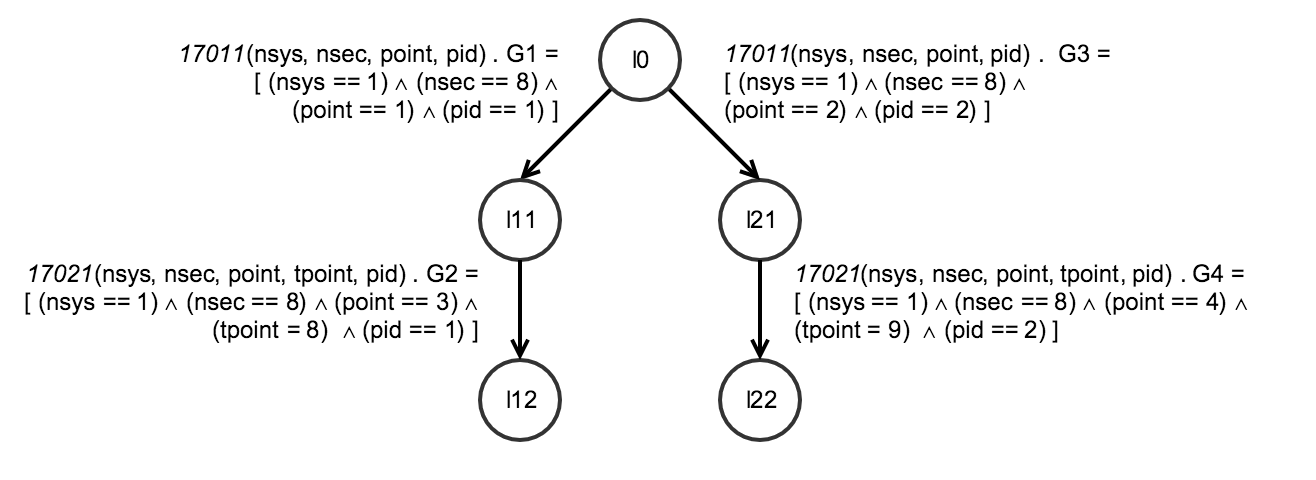
\includegraphics[width=1.0\linewidth]{figures/STS1.png}
    \end{center}

  \caption{First generated Symbolic Transition System model,
  based on the traces given in Figure \ref{fig:tsua}.}
  \label{fig:firstmodel}
\end{figure}
\end{example}

This STS expresses the behaviors found in $Traces(Sua)$ but in a
slightly different manner. Trace inclusion \cite{petrenko06}
between an inferred STS and $Traces(Sua)$, and trace equivalence
\cite{petrenko06} between an inferred STS and $CTraces(Sua)$ are
captured by the following proposition:

\begin{proposition}
    Let $\mathit{Sua}$ be a system under analysis and $Traces(Sua)$ be its
    trace set. $\EuScript{S}_i$ is an inferred STS from
    $Traces(Sua)$.
    We have $Traces(\EuScript{S}_i) = CTraces(Sua) \subseteq Traces(Sua)$.

	\label{def:equivtraces_IOSTS}
\end{proposition}

%%%%%%%%%%%%%%%%%%%%%%%%%%%%%%%%%%%%%%%%%%%%%%%%%%%%%%%%%%%%%%%%

\section{Improving generated models' usability}
\label{sec:modelinf:usability}

The size of the generated models is likely too large to be used
in an efficient manner. That is why we added a reduction step,
described in the next section. Then, we revisit the abstraction
mechanism already introduced in the previous chapter.

\subsection{STS reduction}
\label{sec:modelinf:prodsystems:reduction}

A model $\EuScript{S}_i$ constructed with the steps presented
before is usually too large, and thus cannot be beneficial as is.
Using such a model for testing purpose would lead to too many
test cases for instance. That is why we use a reduction step,
aiming at diminishing the first model into a second one, denoted
by $R(\EuScript{S}_i)$ that is more usable. As discussed in
Chapter \ref{sec:modelinf:webapps}, most of the existing
approaches propose two solutions: (i) inferring models with high
levels of abstraction, which leads to over-approximated models,
(ii) applying a minimization technique, which guarantees trace
equivalence.  Nonetheless, after having investigated this path in
Chapter \ref{sec:modelinf:webapps}, we concluded that
minimization is costly and highly time consuming on large models.

Given that a production system has a finite number of elements
and that there should only be deterministic decisions, the STS
$\EuScript{S}_i$ should contain branches capturing the same
sequences of events (without necessarily the same parameter
assignments).  As a result, we chose to apply an approach
tailored to support large models that consists in combining STS
branches that have the same sequences of actions so that we still
obtain a model having a tree structure. When branches are
combined together, parameter assignments are wrapped into
matrices in such a way that trace equivalence between the first
model and the new one is preserved.  More precisely, a sequence
of successive guards found in a branch is stored into a matrix
column. By doing this, we reduce the model size, we can still
retrieve original behaviors (and only these ones, \emph{i.e.} no
approximation), and we still preserve trace inclusion between the
reduced STS and $Traces(Sua)$.
The use of matrices offers here another advantage: the parameter
assignments are now packed into a structure that can be easily
analyzed later. As shown later in Section
\ref{sec:modelinf:prodsystems:results}, this straightforward
approach gives good results in terms of STS reduction, and
requires low processing time, even with millions of transitions.

Given a STS $\EuScript{S}_i$, every STS branch is adapted to
express sequences of guards in a vector form to ease the STS
reduction. Later, the concatenation of these vectors shall give
birth to matrices. This adaptation is obtained with the
definition of the \emph{STS operator} $Mat$:

\begin{definition}[The $Mat$ operator]
\label{rule:matrix}
  Let $\EuScript{S}_i=<L_{\EuScript{S}_i},l0_{\EuScript{S}_i},V_{\EuScript{S}_i},V0_{\EuScript{S}_i},I_{\EuScript{S}_i},\Lambda_{\EuScript{S}_i},$
  $\rightarrow_{\EuScript{S}_i}>$ be a STS. We denote by
  $Mat(\EuScript{S}_i)$ the \emph{STS operator} that consists in
  expressing guards of STS branches $b_i$ in a vector form, such
  that
  $Mat(\EuScript{S}_i)=<L_{Mat(\EuScript{S}_i)},l0_{Mat(\EuScript{S}_i)},V_{Mat(\EuScript{S}_i)},$
  $V0_{Mat(\EuScript{S}_i)},I_{Mat(\EuScript{S}_i)},\Lambda_{Mat(\EuScript{S}_i)},\rightarrow_{Mat(\EuScript{S}_i)}>$
  where:

	\begin{itemize}
    \item $L_{Mat(\EuScript{S}_i)}=L_{\EuScript{S}_i}$;

    \item $l0_{Mat(\EuScript{S}_i)}=l0_{\EuScript{S}_i}$;

    \item $I_{Mat(\EuScript{S}_i)}=I_{\EuScript{S}_i}$;

    \item $\Lambda_{Mat(\EuScript{S}_i)} = \Lambda_{\EuScript{S}_i}$;

    \item $V_{Mat(\EuScript{S}_i)}$, $V0_{Mat(\EuScript{S}_i)}$,
      and $\rightarrow_{Mat(\EuScript{S}_i)}$ are given by the
      following rule:

    \begin{center}
    {\Large
    $\frac{b_i~= ~l0 \xRightarrow{(a_1(p_1),G_1,A_1) \dots
    (a_n(p_n),G_n,A_n)} l_n}{
      \begin{matrix}
        V0_{Mat(\EuScript{S}_i)}:=V0_{Mat(\EuScript{S}_i)} \wedge
        M_i=\begin{bmatrix}G_1\\ \vdots\\ G_n\end{bmatrix}\\
        l0_{Mat(\EuScript{S}_i)}
        \xRightarrow{(a_1(p_1),M_i[1],id_V) \dots (a_n(p_n),M_i[n],id_V) }_{\rightarrow_{Mat(\EuScript{S}_i)}} l_n\\
      \end{matrix}
    }$
    }
    \end{center}
  \end{itemize}

  Given a branch $b_i \in (\rightarrow_{Mat(\EuScript{S}_i)})^n$,
  we also denote by $Mat(b_i) = M_i$ the vector used with $b_i$.
\end{definition}

It is now possible to merge the STS branches that have the same
sequences of actions. This last sentence can be interpreted as an
equivalence relation over STS branches from which we can derive
\emph{equivalence classes}:

\begin{definition}[STS branch equivalence class]
Let
$\EuScript{S}_i=<L_{\EuScript{S}_i},l0_{\EuScript{S}_i},V_{\EuScript{S}_i},V0_{\EuScript{S}_i},I_{\EuScript{S}_i},$
$\Lambda_{\EuScript{S}_i}, \rightarrow_{\EuScript{S}_i}>$ be a STS obtained from
$Traces(Sua)$ (and having a tree structure).

$[b]$ denotes the \emph{equivalence class} of $\EuScript{S}_i$
branches such that: $[b]=\{
    b_j = l0_{\EuScript{S}_i}\\ \xRightarrow{(a_1(p_1),G_{1j},A_{1j}) \dots
    (a_n(p_n),G_{nj},A_{nj})}
    l_{nj} (1 \leq j) \mid b = l0_{\EuScript{S}_i}
    \xRightarrow{(a_1(p_1),G_{1},A_{1})\dots(a_n(p_n),G_{n},A_{n})} l_n\}.$
\end{definition}

The reduced STS denoted by $R(\EuScript{S}_i)$ of
$\EuScript{S}_i$ is obtained by concatenating all the branches of
each equivalence class $[b]$ found in $Mat(\EuScript{S}_i)$ into
one branch. This is achieved by an algorithm based on hashes (cf.
Section \ref{sec:prodsystems:impl-exp-collect}). The vectors
found in the branches of $[b]$ are concatenated as well into the
same unique matrix $M_{[b]}$. A column of this matrix represents
a complete and ordered sequence of guards found in one initial
branch of $\EuScript{S}_i$. $R(\EuScript{S}_i)$ is defined as
follows:

\begin{definition}[Reduced STS $R(\EuScript{S}_i)$]
	\label{rule:min}

	Let $\EuScript{S}_i=<L_{\EuScript{S}_i},l0_{\EuScript{S}_i},V_{\EuScript{S}_i},V0_{\EuScript{S}_i},I_{\EuScript{S}_i},\Lambda_{\EuScript{S}_i},$ $\rightarrow_{\EuScript{S}_i}>$ be
    a STS inferred from a structured trace set $Traces(Sua)$. The
    reduction of $\EuScript{S}_i$ is modeled by the STS
    $R(\EuScript{S}_i)=
    <L_R,l0_R,V_R,V0_R,I_R,\Lambda_R,\rightarrow_R>$ where:

  \begin{center}
      {\Large
  $\frac{\begin{matrix}
      [b]=\{b_1, \dots ,b_m\},
      b=l0_{\EuScript{S}_i} \xRightarrow{(a_1(p_1),G_{1},A_{1})
      \dots (a_n(p_n),G_{n},A_{n})} l_{n}\\
      % TODO: I removed: _{Mat(\EuScript{S}_i)} from \xRightarrow{}
    \end{matrix}
  }
  {\begin{matrix}
      V0_R:=V0_R \wedge M_{[b]}=[Mat(b_1), \dots ,Mat(b_m)] \wedge (1 \leq c_{[b]} \leq m),\\
      l0_R \xRightarrow{(a_1(p_1),M_{[b]}[1,c_{[b]}],id_V) \dots
      (a_n(p_n),M_{[b]}[n,c_{[b]}],id_V)}_{\rightarrow_R} (l_{n1}
      \cdots l_{nm})
    \end{matrix}
  }$
  }
  \end{center}
\end{definition}

The resulting model $R(\EuScript{S}_i)$ is a STS composed of
variables assigned to matrices whose values are used as guards. A
matrix column represents a successive list of guards found in a
branch of the initial STS $\EuScript{S}_i$. The choice of the
column in a matrix depends on a new variable $c_{[b]}$.

\begin{example}
Figure \ref{fig:reduced-model} depicts the reduced model obtained
from the STS depicted in Figure \ref{fig:firstmodel}. Its guards
are placed into two vectors
$M_1=\begin{bmatrix}G1\\G2\end{bmatrix}$ and
$M_2=\begin{bmatrix}G3\\G4\end{bmatrix}$, combined into the same
matrix $M_{[b]}$. The variable $c_{[b]}$ is used to take
either the guards of the first column or the guards of the
second one.

\begin{figure}[h]
    \begin{center}
        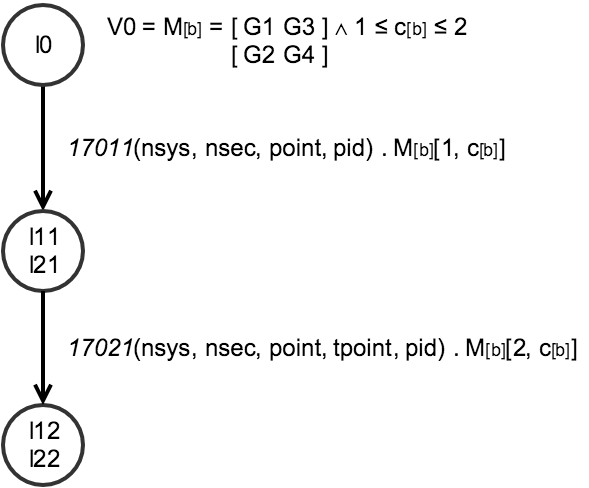
\includegraphics[width=0.6\linewidth]{figures/STS2.png}
    \end{center}

	\caption{Reduced Symbolic Transition System model obtained
    from the model depicted in Figure \ref{fig:firstmodel}.}
	\label{fig:reduced-model}
\end{figure}
\end{example}

The STS $R(\EuScript{S}_i)$ has less branches but still expresses
the initial behaviors described by the STS $\EuScript{S}_i$.
$R(\EuScript{S}_i)$ and $\EuScript{S}_i$ are said trace
equivalent \cite{petrenko06}.  This is captured by the following
proposition:

\begin{proposition}
  Let $\mathit{Sua}$ be a system under analysis and $Traces(Sua)$ be its traces
  set. $R(\EuScript{S}_i)$ is a STS derived from $Traces(Sua)$.
  We have $Traces(R(\EuScript{S}_i)) = Traces(\EuScript{S}_i) =
  CTraces(Sua) \subseteq Traces(Sua)$.
\end{proposition}

\subsection{STS abstraction}

Given the trace set $ST_i \in CTraces(Sua)$, the generated STS
$R(\EuScript{S}_i)$ can be used for analysis purpose, but it is still
difficult to manually interpret, even for experts.  This fifth
\textit{Autofunk} module aims to analyze $R(\EuScript{S}_i)$ in
order to produce a new STS $\EuScript{S}_i^\uparrow$ whose level
of abstraction is lifted by using more intelligible actions. This
process is performed with inference rules, which encode the
knowledge of the expert of the system. These rules are fired on
the transitions of $R(\EuScript{S}_i)$ to deduce new transitions.
We consider the same two types of rules as in
\crossref{sec:modelinf:webapps}{sec:modelinf:webapps:L4}:

\begin{itemize}
    \item The rules \emph{replacing some transitions} by more
    comprehensive ones. These rules are of the form: \textit{When
    Transition $l_1 \xrightarrow{a(p),G,A}_{R(\EuScript{S}_i)}
    l_2$, condition on $a(p),G,A$, Then add $l_1
    \xrightarrow{a'(p'),G',A'}_{\EuScript{S}_i^\uparrow} l_2$ and
    retract $l_1 \xrightarrow{a(p),G,A}_{R(\EuScript{S}_i)}
    l_2$};

    \item The rules that \emph{aggregate some successive transitions}
    to a single transition compound of a more abstract action.
    These rules are of the form \textit{When Transition $l_1
    \xRightarrow{(a_1,G_1,A_1),...(a_n,G_n,A_n)} l_n$, condition
    on $(a_1,G_1,A_1),...(a_n,G_n,A_n)$, Then add $l_1
    \xrightarrow{a(p),G,A}_{\EuScript{S}_i^\uparrow} l_n $, and
    retract $l_1 \xRightarrow{(a_1,G_1,A_1),...(a_n,G_n,A_n)} l_n$}.
\end{itemize}

The generated STSs represent recorded scenarios modeled at a
higher level of abstraction. These can be particularly useful for
generating documentation or better understanding how the system
behaves, especially when issues are experienced in production.
On the other hand, it is manifest that the trace inclusion
property is lost with the STSs constructed by this module because
sequences are modified. In other words, such models cannot be
used for testing purpose.

\begin{example}
If we take back our example, the actions of the STS depicted in
Figure \ref{fig:reduced-model} can be replaced thanks to the
inference rules given in Figure \ref{rule:rename-tr}. Such rules
change the labels $17011$ and $17021$ to more intelligible ones.
The STS depicted on the left in Figure \ref{fig:finalmodel} is
the result of the application of these rules on the model given
in Figure \ref{fig:reduced-model}.
The rule shown in Figure \ref{rule:aggregate-tr} aggregates
two transitions into a unique transition indicating the movement
of a product in its production line. $Transition$ are facts
modeling STS transitions as seen in Chapter
\ref{sec:modelinf:webapps}. We need a variable $\$lfinal$ that
retains the final location of the first transition $\$t1$, so
that we can reuse it in the condition of the second transition
$\$t2$. The final location of the first transition must be the
initial location of the second transition ($Linit == \$lfinal$)
to perform the aggregation. From 5 initial production events
that are not self-explanatory, we generate a simpler STS
constituted of one transition, clearly expressing a part of the
functioning of the system. The result of this rule is shown in
Figure \ref{fig:finalmodel} (on the right).
\end{example}

\begin{figure}[ht]
\begin{framed}
\begin{BVerbatim}
rule "Mark destination requests"
when:
  $t: Transition(action == "17011")
then
  $t.setAction("DestinationRequest")
end
\end{BVerbatim}
\end{framed}

\begin{framed}
\begin{BVerbatim}
rule "Mark destination responses"
when:
  $t: Transition(action == "17021")
then
  $t.setAction("DestinationResponse")
end
\end{BVerbatim}
\end{framed}

  \caption{Two rules adding value to existing transitions by
  replacing their actions by more intelligible ones. These names
  are part of the domain language used by Michelin experts.}
  \label{rule:rename-tr}
\end{figure}

\begin{figure}[ht]
\begin{framed}
\begin{BVerbatim}
rule "Aggregate destination requests/responses"
when
  $t1: Transition(
    action == "DestinationRequest", $lfinal := Lfinal
  )
  $t2: Transition(
    action == "DestinationResponse" , Linit == $lfinal
  )
then
  insert(
    new Transition(
      "ProductAdvance",
      Guard($t1.Guard, $t2.Guard),
      Assign($t1.Assign, $t2.Assign),
      $t1.Linit,
      $t2.Lfinal
    )
  )
  retract($t1)
  retract($t2)
end
\end{BVerbatim}
\end{framed}

  \caption{An inference rule that aggregates two transitions of a
  Symbolic Transition System into a single transition. An example
  of its application is given in Figure \ref{fig:finalmodel}.}
  \label{rule:aggregate-tr}
\end{figure}

\begin{figure}[ht]
    \begin{center}
        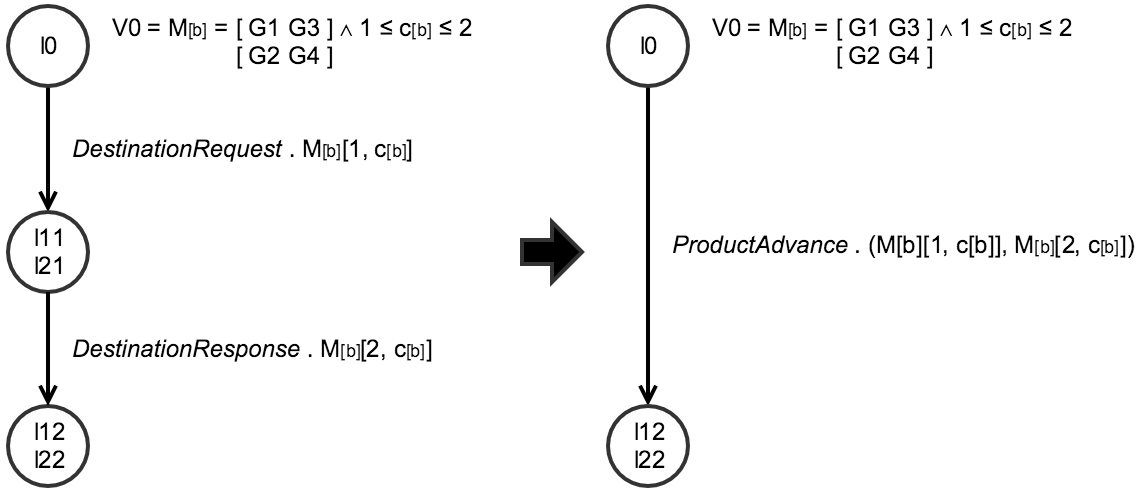
\includegraphics[width=1.0\linewidth]{figures/STSfinal.png}
    \end{center}

    \caption{The construction of the final Symbolic Transition
    System model. The final model is on the right, obtained after
    having applied all the abstraction rules given in Figures
    \ref{rule:rename-tr} and \ref{rule:aggregate-tr}.}
	\label{fig:finalmodel}
\end{figure}

% By writing 20 rules to enrich the meaning of the actions for our
% case study with Michelin, we were able to generate a model that
% Michelin experts understood. We then wrote 6 more rules to
% aggregate sequences of transitions in order to generate reduced
% models, mimicking some of the existing Michelin specifications.

%%%%%%%%%%%%%%%%%%%%%%%%%%%%%%%%%%%%%%%%%%%%%%%%%%%%%%%%%%%%%%%%%

\section{Implementation and experimentation}
\label{sec:modelinf:prodsystems:results}

In this section, we briefly describe the implementation of our
model inference framework for Michelin. Then, we give an
evaluation on real production systems.

\subsection{Implementation}
\label{sec:prodsystems:impl-exp-collect}

Our framework \textit{Autofunk v2} is developed in Java and
leverages Drools.  In our industrial context, we have several
bases of facts used throughout the different \textit{Autofunk}
modules, represented as Java objects such as: Events, Trace sets
$ST_i$, Runs, Transitions, and STSs. We chose to target
performance and simplicity while implementing \textit{Autofunk}.
That is why most of the steps are implemented with parallel
algorithms (except the production event parsing). Figure
\ref{fig:autofunk_initial_setup} shows the initial setup of
\textit{Autofunk}. We have sets of log files to parse coming from
Michelin's logging system. \textit{Autofunk} reads these files,
and transforms them into traces, that are then used to build
models.

\begin{figure}[ht]
    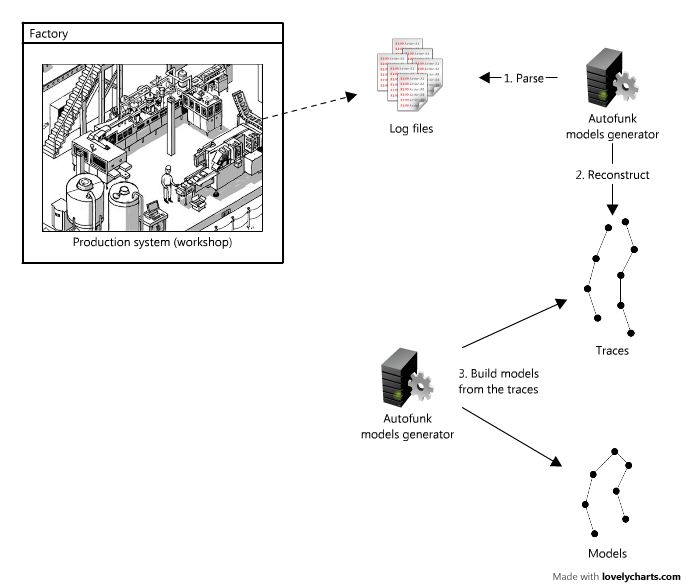
\includegraphics[width=1.0\linewidth]{figures/autofunk_initial_setup.png}

    \caption{The architecture of \textit{Autofunk} that has been
        used to conduct our first experiments with Michelin log
        files. A newer (and better) architecture is given in
        Figure \ref{fig:autofunk_gen_branded}.}
    \label{fig:autofunk_initial_setup}
\end{figure}

The input trace collection is constructed with a classical
parser, which returns $Event$ Java objects. By now, we are not
able to parallelize this part because of an issue we faced with
Michelin's logging system. The resulting drawback is that the
time to parse traces is longer than expected and heavily depends
on the size of data to parse. The $Event$ base is then filtered
with Drools inference rules as presented in Section
\ref{part3:collecting}.  Then, we call a straightforward
algorithm for reconstructing traces: it iterates over the $Event$
base and creates a set for each assignment of the identifier
$pid$. These sets are sorted to construct traces given as $Trace$
Java objects. These objects correspond to $Traces(Sua)$. The
generation of the trace subsets $ST= \{ST_1,...,ST_N\}$ and of
the first STSs are done with Drools inference rules applied in
parallel.

The STS reduction, and specifically the generation
of STS branches equivalence classes, has been implemented with a
specific algorithm for better performance. Indeed, comparing
every action in STS branches in order to aggregate them is time
consuming.  Given a STS $\EuScript{S}$, this algorithm generates
a signature for each branch $b$, \emph{i.e.} a hash
(SHA1\footnote{Secure Hash Algorithm 1} algorithm) of
the concatenation of the signatures of the actions of $b$. The
branches which have the same signature are gathered together and
establish branch equivalence classes (as described in Section
\ref{sec:modelinf:prodsystems:reduction}). Implementing
equivalence classes using hashes allows to quickly reduce STS of
any size, especially because this technique scales well.
Thereafter, the reduced $R(\EuScript{S})$ is constructed thanks
to the inference rule given in Section
\ref{sec:modelinf:prodsystems:reduction}.

At the time of writing, we are working on the architecture
depicted in Figure \ref{fig:autofunk_gen_branded}. It shows how
we plan to integrate \textit{Autofunk} with any Michelin
production system.  Events are collected on-the-fly from a system
under analysis, and sent to a database
(Elasticsearch\footnote{\url{https://www.elastic.co/products/elasticsearch}}
here) thanks to a message broker (namely
RabbitMQ\footnote{\url{https://www.rabbitmq.com/}}). Initial
benchmarks revealed that such an infrastructure allows to collect
up to 10,000 events per second with a negligible overhead on the
system. \textit{Autofunk} then queries the database to fetch
product events, and finally build models. This approach also
solves the issue mentioned previously. Furthermore, it allows to
leverage the data for other purposes, \emph{e.g.}, visualization or more
extensive analyses.

\begin{figure}[ht]
    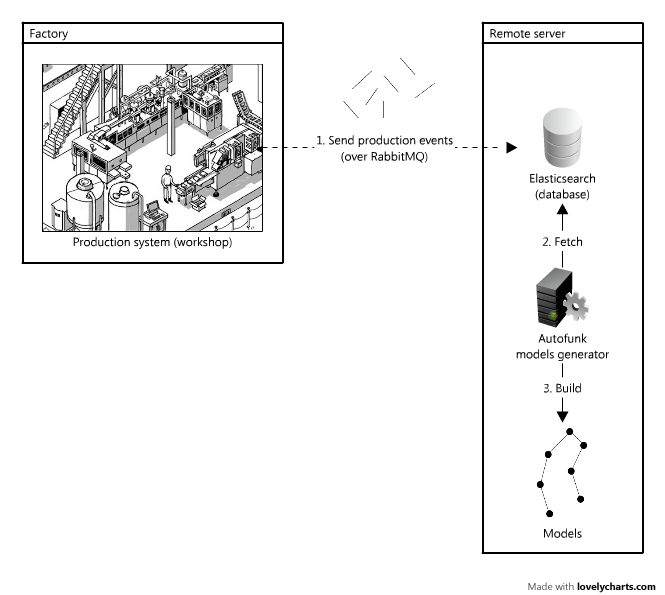
\includegraphics[width=1.0\linewidth]{figures/model-gen-branded.png}

    \caption{The overall architecture built at Michelin to use
    \textit{Autofunk} in a production environment. Events are
    sent over RabbitMQ to another server in order to minimize
    the overhead. Collected events are stored in a database.
    \textit{Autofunk} can then fetch these events, and build
    the models.}
    \label{fig:autofunk_gen_branded}
\end{figure}

\subsection{Evaluation}

We conducted several experiments with real sets of production
events, recorded in one of Michelin's factories at different
periods of time. We executed our implementation of \emph{Autofunk
v2} on a Linux (Debian) machine with 12 Intel(R) Xeon(R) CPU
X5660 @ 2.8GHz and 64GB RAM.

We present here the results of 6 experiments on the same
production system with different event sets collected during 1,
8, 11, 20, and 23 days. These results are depicted in Table
\ref{fig:results}. The third column gives the number of
production events recorded on the system. The next column shows
the trace number obtained after the parsing step.  $N$ and $M$
represent the entry and exit points automatically computed with
the statistical analysis. The column Trace Subsets shows how
$Traces(Sua)$ is segmented into subsets $\{ST_1,\dots,ST_N\}$ and
the number of traces included in each subset. These numbers of
traces also correspond to the numbers of branches generated in
the STSs $\EuScript{S}_1,\dots,\EuScript{S}_N$. The eighth column,
\# $R(\EuScript{S}_i)$, represents the number of branches found
in each reduced STSs $R(\EuScript{S}_1),\dots,R(\EuScript{S}_N)$.
Finally, execution times are rounded and expressed in minutes in
the last column.

\begin{sidewaystable}
\begin{center}
\begin{tabular}{| c | c | c | c | c | c | c | c | c | c | c |}
\hline
Experiment & Number of days & Number of events &
$Card(Traces(Sua))$ & $N$ & $M$ & \# Trace subsets & \#
$R(\EuScript{S}_i)$ & Exec. time (min)\\
\hline
\hline
$A_1$ & 1     & 660,431   & 16,602  & 2 & 3 & 4,822  & 332   & 1 \\
$A_2$ &       &           &         &   &   & 1,310  & 193   &   \\
\hline
$B_1$ & 8     & 3,952,906 & 66,880  & 3 & 3 & 28,555 & 914   & 9 \\
$B_2$ &       &           &         &   &   & 18,900 & 788   &   \\
$B_3$ &       &           &         &   &   &  6,681 &  51   &   \\
\hline
$C_1$ & 11    & 3,615,215 & 61,125  & 3 & 3 & 28,302 & 889   & 9 \\
$C_2$ &       &           &         &   &   & 14,605 & 681   &   \\
$C_2$ &       &           &         &   &   &  7,824 &  80   &   \\
\hline
$D_1$ & 11    & 3,851,264 & 73,364  & 2 & 3 & 35,541 & 924   & 9 \\
$D_2$ &       &           &         &   &   & 17,402 & 837   &   \\
\hline
$E_1$ & 20    & 7,635,494 & 134,908 & 2 & 3 & 61,795 & 1,441 & 15 \\
$E_2$ &       &           &         &   &   & 35,799 & 1,401 &    \\
\hline
$F_1$ & 23    & 9,231,160 & 161,035 & 2 & 3 & 77,058 & 1,587 & 21 \\
$F_2$ &       &           &         &   &   & 43,536 & 1,585 &    \\
\hline
\end{tabular}
\end{center}

\caption{This table shows the results of 6 experiments on a
Michelin production system with different event sets.}
\label{fig:results}
\end{sidewaystable}

First, these results show that our framework can take millions of
production events and still builds models quickly (20 minutes).
With sets collected during one day up to one week (experiments
$A$, $B$, $C$, and $D$), models are inferred in less than 10
minutes. Hence, \textit{Autofunk} can be used to quickly infer
models for analysis purpose or to help diagnose faults in a
system. Experiment $F$ handled almost 10 million events in less
than half an hour to build two models including around 1,600
branches. As mentioned earlier in this section, the parsing
process is not parallelized yet, and it took up to 20 minutes to
open and parse around 1,000 files (number of Michelin log files
for this experiment). This issue is solved by the architecture
presented in Figure \ref{fig:autofunk_gen_branded}.  The graph
shown in Figure \ref{fig:time-vs-messages} summarizes the
performances of our framework, and how fast it is at transforming
production events into models (experiments $B$, $C$ and $D$ run
in about 9 minutes). It also demonstrates that doubling the event
set does not involve doubling its execution time. The linear
regression reveals that the overall framework scales well, even
with the current parsing implementation.

In Table \ref{fig:results}, the difference between the number of
trace subsets (7th column) and the number of branches included in
the STSs $R(\EuScript{S}_i)$ (8th column) clearly shows that our
STS reduction approach is effective. For instance, with
experiment $B$, we reduce the STSs by 91.88\% against the initial
trace set $Traces(Sua)$. In other words, 91\% of the original
behaviors are packed into matrices. As a reminder, such results
are tied to the specific context of Michelin production systems.
The reduction ratio may vary with other systems.

\begin{figure}[ht]
  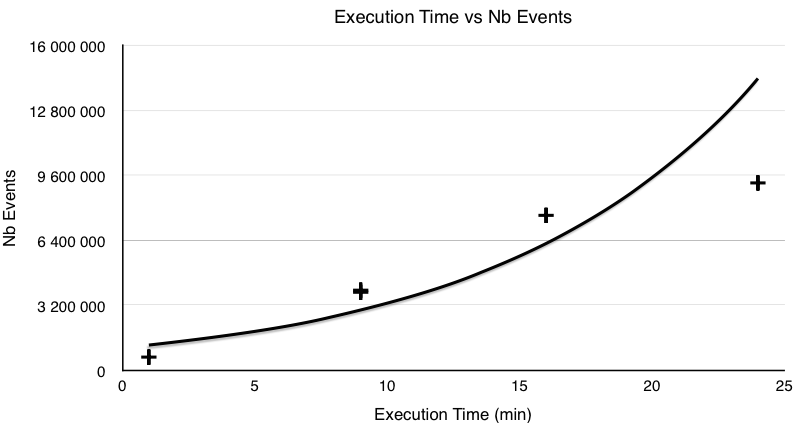
\includegraphics[width=1.0\linewidth]{figures/time-vs-messages.png}

  \caption{Execution time vs events. According to the trend shown
  by the linear regression, we can state that our framework
  scales well.}
  \label{fig:time-vs-messages}
\end{figure}

We also extracted the values of columns 4 and 7 in Table
\ref{fig:results} to depict the stacked bar chart illustrated in
Figure \ref{fig:proportions}. This chart shows, for each
experiment, the proportion of complete traces kept by
\textit{Autofunk} to build models, over the initial number of
traces in $Traces(Sua)$.  \textit{Autofunk} has kept only 37\% of
the initial traces in Experiment $A$ because its initial trace
set is too small and contains many incomplete behaviors. During a
day, most of the recorded traces do not start or end at entry or
exit points, but rather start or end somewhere in production
lines (cf. Section \ref{prodsys:context}). That is why, on a
single day, we can find so many incomplete traces. With more
production events, such a phenomenon is limited because we absorb
these storage delays.

\begin{figure}[ht]
  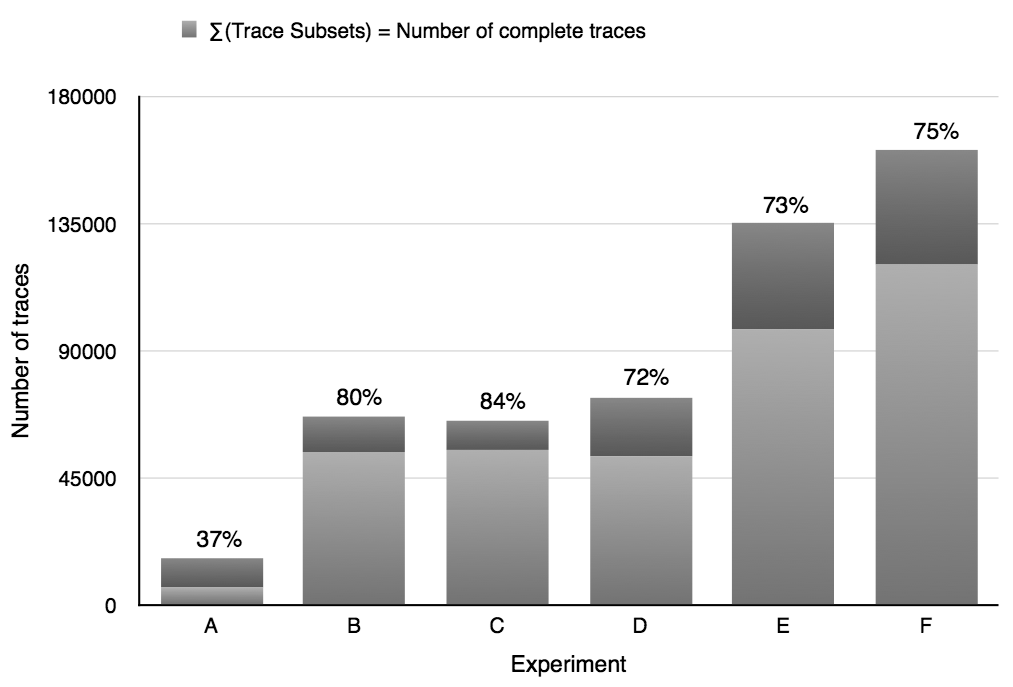
\includegraphics[width=1.0\linewidth]{figures/proportions.png}

  \caption{Proportions of complete traces for the different
  experiments. This chart shows that \textit{Autofunk} considers
  a lot of traces to infer models, but there is still room for
  improvement.}
  \label{fig:proportions}
\end{figure}

We can also notice that experiments $C$ and $D$ have similar
initial trace sets but experiment $C$ owns more complete traces
than experiment $D$ by 12\%, which is significant. Furthermore, experiments
$B$ and $C$ take 3 entry points into account while the others only
take 2 of them. This is related to the fixed limit of 10\% we
chose to ensure truly entry points to be automatically selected.
The workshop we analyzed has three entry points whose two are
mainly used. The third entry point is employed to balance the
production load between this workshop and a second one located
close to it in the same factory. Depending on the period, this
entry point may be more or less solicited, hence the
difference between experiments $B$, $C$ and experiment $D$.
Increasing the limit of 10\% to a higher value would change the value
of $N$ for experiments $B$ and $C$, but would also impact
experiment $A$ by introducing false results since incorrect entry
points could be selected. By means of a manual analysis, we
concluded that 10\% was the best ratio for removing incomplete
traces in our experiments.  30\% of initial traces have been
removed, which is close to the reality.

Another potential issue with our parsing implementation is that
every event has to be loaded in memory, so that we can perform
computation and apply our algorithms on them. But working
with millions of Java objects requires a lot of memory, \emph{i.e.}
memory consumption depends on the amount of initial traces. We
compared execution time and memory consumption in Figure
\ref{fig:memory-time}, showing that memory consumption tends to
follow a logarithmic trend. In the next version of
\textit{Autofunk}, we plan to work on improving memory
consumption even if it has been considered acceptable as is by
Michelin.

\begin{figure}[ht]
  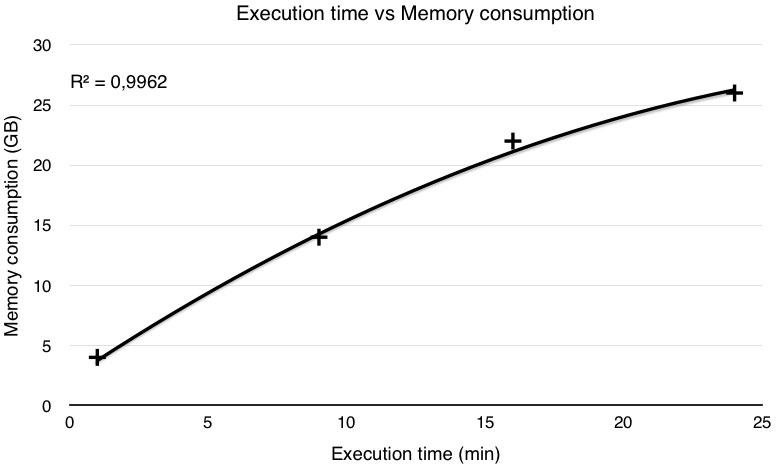
\includegraphics[width=1.0\linewidth]{figures/memory-time.png}

  \caption{Execution time vs memory consumption. This version 2 of
  \textit{Autofunk} is still a prototype, and memory consumption
  remains an issue.}
  \label{fig:memory-time}
\end{figure}

For confidentiality reasons, we are not able to provide results
related to the generation of more abstract models.

%%%%%%%%%%%%%%%%%%%%%%%%%%%%%%%%%%%%%%%%%%%%%%%%%%%%%%%%%%%%%%%%%

\section{A better solution to the trace segmentation and
filtering problem with machine learning}
\label{sec:modelinf:prodsystems:better-segmentation}

In Section \ref{sec:modelinf:prodsystems:segmentation}, we
presented a statistical analysis to segment and filter the
initial trace set used to infer models, part of \emph{Autofunk
v2}. Nevertheless, experiments (as seen in the previous section)
revealed that this empirical method was not stable, in other
words the use of a configurable minimum limit was not accurate
enough. That is why we chose to work on a new solution to segment
and filter traces, which gave birth to \emph{Autofunk v3}.

\emph{Autofunk v3} now relies on a \emph{machine learning}
technique to segment a trace set into several subsets, one per
entry point of the system $\mathit{Sua}$. We leverage this
process to also remove incomplete traces, \emph{i.e.} traces that
do not express an execution starting from an entry point and
ending to an exit point. These can be extracted by analyzing the
traces and the variable $point$, which captures the product
physical location.

In order to determine both entry and exit points of
$\mathit{Sua}$, we rely on an outlier detection approach
\cite{1695852}. An outlier is an observation that deviates so
much from the other observations as to arouse suspicions that it
was generated by a different mechanism. More precisely, we chose
to use the \emph{k-means clustering} method
\cite{10.2307/2346830}, a machine learning algorithm, which is
both fast and efficient, and does not need to be trained before
being effectively used (that is called unsupervised learning, and
it is well-known in the machine learning field). \textit{k-means
clustering} aims to partition $n$ observations into $k$ clusters
as shown in Figure \ref{fig:kmeans}.

\begin{figure}[ht]
    \begin{center}
        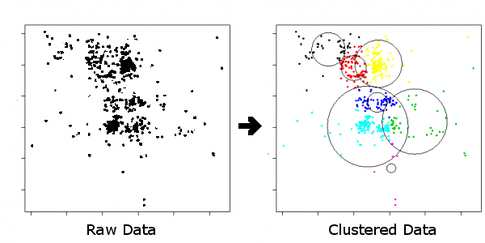
\includegraphics[width=1.0\linewidth]{figures/kmeans.png}
    \end{center}

    \caption{k-means clustering explained: the intuition is to
    partition $n$ observations into $k$ clusters in which each
    observation belongs to the cluster with the nearest mean.}
    \label{fig:kmeans}
\end{figure}

In our context, observations are represented by the variable
$point$ present in each trace of $Traces({Sua})$, which captures
the product physical location, and $k=2$ as we want to group the
outliers together, and leave the other points in another cluster.
But, since we want to leverage the largest part of the initial
trace set, we apply \textit{k-means clustering} several times
until reaching 80\% of traces retained in a cluster.

Once the entry and exit points are found, we segment
$Traces({Sua})$ and obtain a set $CTraces({Sua})=\{ST_1, \dots,
ST_n\}$. Then, we apply the same generation and reduction steps
as described in Section \ref{sec:modelinf:prodsystems:generation}
and Section \ref{sec:modelinf:prodsystems:reduction} so that we
obtain the reduced model $R(\EuScript{S}) =
\{R(\EuScript{S}_1),\dots,R(\EuScript{S}_n)\}$.

%%%%%%%%%%%%%%%%%%%%%%%%%%%%%%%%%%%%%%%%%%%%%%%%%%%%%%%%%%%%%%%%%

\section{Conclusion}
\label{sec:modelinf:prodsystems:conclusion}

In this chapter, we presented our revisited framework
\textit{Autofunk}, combining model inference, machine learning,
and expert systems to generate models from production systems.
Figure \ref{fig:autofunk_branded} shows the final architecture of
our \emph{third} version of \textit{Autofunk} along with the
technologies used in each module. Given a large set of production
events, our framework infers exact models whose traces are
included in the initial trace set of a system under analysis
\cite{petrenko06}.  We chose to design \textit{Autofunk} for
targeting high performance. Our evaluation shows that this
approach is suitable in the context of production systems since
we quickly obtain STS trees reduced by 90\% against the original
trace sets of the system under analysis.

\begin{figure}[h]
    \begin{center}
        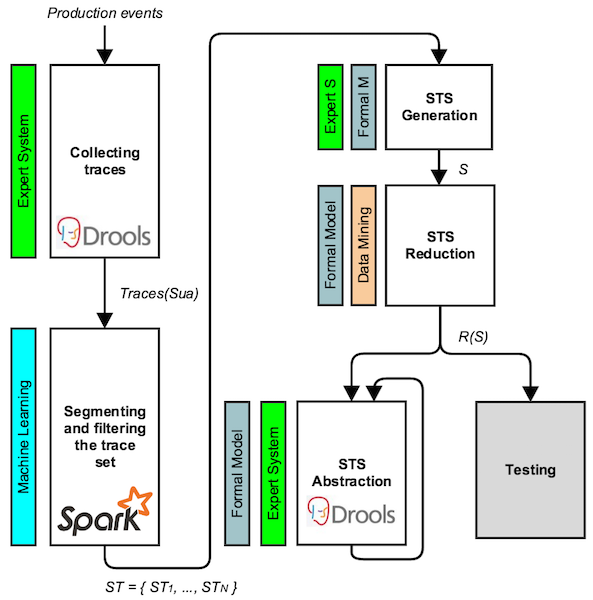
\includegraphics[width=1.0\linewidth]{figures/autofunk_branded.png}
    \end{center}

    \caption{Final architecture of our framework
    \textit{Autofunk} (v3), designed for quickly inferring
    models of Michelin's production systems.}
    \label{fig:autofunk_branded}
\end{figure}

While there is still room for improvement on how we generate
exact models, we decided to go deeper and use such models for
testing purpose. In the next chapter, we describe our testing
technique that leverages the work presented in this chapter.


% !TEX root = ../../thesis.tex
%
\chapter{Testing applied to production systems}
\label{sec:testing}

\TODO{intro}

\section{Offline passive testing}
\label{sec:testing:offpassive}




\section{Online passive testing}
\label{sec:testing:onpassive}

\section{Active testing}
\label{sec:testing:active}

% !TEX root = ../../thesis.tex
%
\chapter{Conclusion}
\label{sec:conclusion}

\Blindtext[2][1]

\section{System Section 1}
\label{sec:conclusion:sec1}

\Blindtext[2][2]

\section{System Section 2}
\label{sec:conclusion:sec2}

\Blindtext[3][2]

\section{Future Work}
\label{sec:conclusion:future}

\Blindtext[2][2]


\cleardoublepage

% --------------------------
% Back matter
% --------------------------
{%
\setstretch{1.1}
\renewcommand{\bibfont}{\normalfont\small}
\setlength{\biblabelsep}{0pt}
\setlength{\bibitemsep}{0.5\baselineskip plus 0.5\baselineskip}
\printbibliography[nottype=online]
\printbibliography[heading=subbibliography,title={Webseiten},type=online,prefixnumbers={@}]
}
\cleardoublepage

\listoffigures
\cleardoublepage

\listoftables
\cleardoublepage

% !TEX root = ../thesis.tex
%
\pagestyle{empty}
\hfill
\vfill
\pdfbookmark[0]{Colophon}{Colophon}
\section*{Colophon}

This thesis was typeset with \LaTeXe.
It uses the \textit{Clean Thesis} style developed by Ricardo Langner.
The design of the \textit{Clean Thesis} style is inspired by user guide documents from Apple Inc.

Download the \textit{Clean Thesis} style at \url{http://cleanthesis.der-ric.de/}.

\cleardoublepage

%% !TEX root = ../thesis.tex
%
%************************************************
% Declaration
%************************************************
\pdfbookmark[0]{Declaration}{Declaration}
\chapter*{Declaration}
\label{sec:declaration}
\thispagestyle{empty}

You can put your declaration here, to declare that you have
completed your work solely and only with the help of the
references you mentioned.

\bigskip

\noindent\textit{\thesisUniversityCity, \thesisDate}

\smallskip

\begin{flushright}
	\begin{minipage}{5cm}
		\rule{\textwidth}{1pt}
		\centering\thesisName
	\end{minipage}
\end{flushright}

%*****************************************
%*****************************************

%\clearpage
%\newpage
%\mbox{}

% **************************************************
% End of Document CONTENT
% **************************************************
\end{document}
